\subsection{Question 1}
	In this case $\epsilon_k: 2 \times 1$, $\delta_k:$ scalar. In the general case, $\epsilon_k$ will be $N \times 1$, where $N$ is
	the number of state variables, and $\delta_k$ will be $M \times 1$, where $M$ is the number of variables the EKF tries to estimate.
	\\
	A scalar Gaussian is characterized by a mean value $\mu$ and a variance $\sigma^2$. A white Gaussian has $\mu = 0$.
	In the general case, $\boldsymbol{\mu}$ is a single-column matrix and the scalar variance is replaced by a covariance matrix
	$\boldsymbol{\Sigma}$. In this case, a white Gaussian has $\boldsymbol{\mu} = \boldsymbol{0}$ and $\boldsymbol{\Sigma}$ is a
	diagonal matrix because the noise in each state variable is independent of one another.

\subsection{Question 2}

\begin{table}[!htb]
	\centering
    \begin{tabular}{l|l}
    Variable & Usage                                                    \\ \hline
    $x$        & The true state of the system.							  \\
    $\hat{x}$  & The estimate of the true state of the system by the EKF.\\
    $P$        & Estimate error covariance matrix.                       \\
    $G$        & Identity matrix for dimensionality consistency.          \\
    $D$        & Identity matrix for dimensionality consistency. Scalar here. \\
    $Q$        & Measurement noise variance.         \\
    $R$        & Process noise covariance matrix.                    \\
    $wStdP$    & The actual (simulated) standard deviation of the noise in position.            \\
    $wStdV$    & The actual (simulated) standard deviation of the noise in velocity.            \\
    $vStd$     & The actual (simulated) standard deviation of the noise in position estimation. \\
    $u$        & Control signal, the acceleration.                       \\
    $PP$       & Estimate error covariances over time.                              \\
    \end{tabular}
\end{table}


\subsection{Question 3}

\begin{figure}[H]
	\scalebox{0.5}{% This file was created by matlab2tikz.
%
%The latest updates can be retrieved from
%  http://www.mathworks.com/matlabcentral/fileexchange/22022-matlab2tikz-matlab2tikz
%where you can also make suggestions and rate matlab2tikz.
%
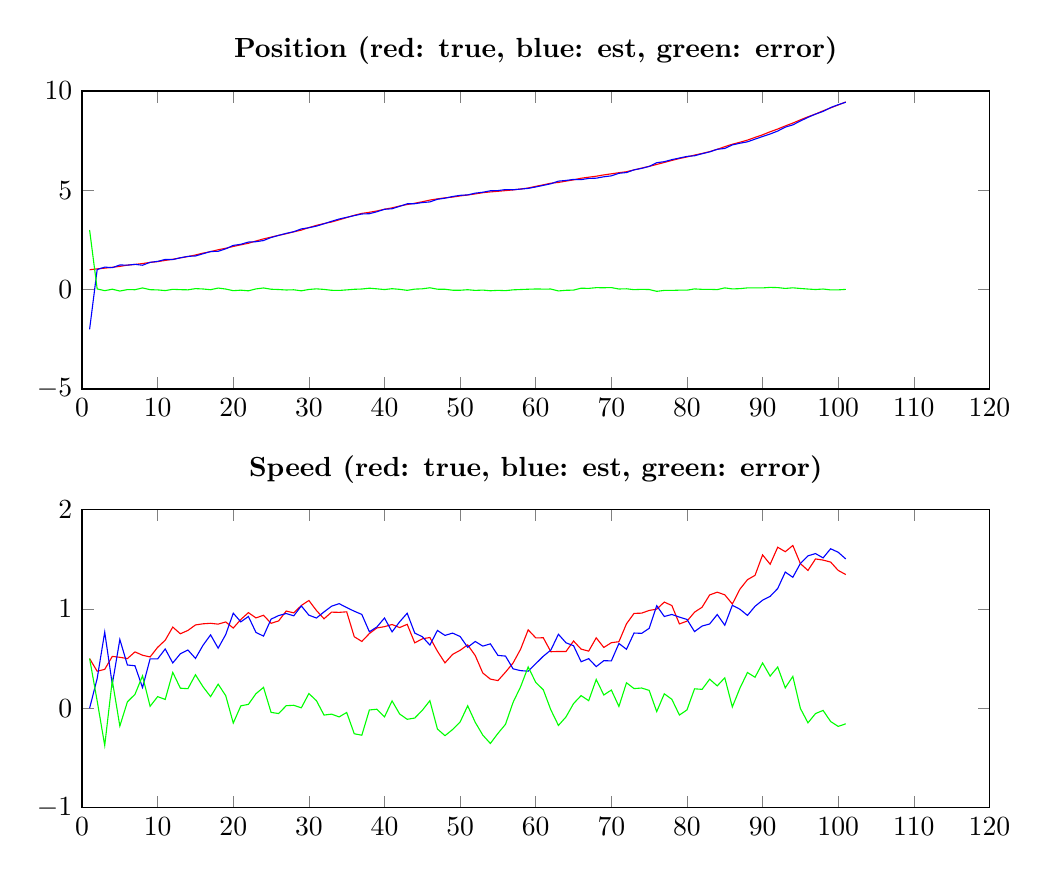
\begin{tikzpicture}

\begin{axis}[%
width=4.537in,
height=1.49in,
at={(0.761in,2.579in)},
scale only axis,
xmin=0,
xmax=120,
ymin=-5,
ymax=10,
axis background/.style={fill=white},
title style={font=\bfseries},
title={Position (red: true, blue: est, green: error)}
]
\addplot [color=red,solid,forget plot]
  table[row sep=crcr]{%
1	1\\
2	1.04479067112728\\
3	1.07990359937776\\
4	1.12479678798294\\
5	1.16833962549014\\
6	1.23261581369435\\
7	1.26739060310157\\
8	1.31231238590902\\
9	1.36996616890753\\
10	1.40798584109908\\
11	1.47013089623621\\
12	1.52790593641987\\
13	1.59883946886639\\
14	1.66308894258421\\
15	1.74292637630064\\
16	1.83684418197805\\
17	1.91198620579175\\
18	2.00762507338724\\
19	2.08131083936684\\
20	2.17278233066961\\
21	2.25421975586445\\
22	2.33243946787947\\
23	2.44688320051738\\
24	2.5539879572573\\
25	2.64196929850894\\
26	2.73337499947702\\
27	2.81307212041001\\
28	2.90830403131994\\
29	2.99542971701437\\
30	3.1235786080139\\
31	3.23403750725304\\
32	3.32582642860213\\
33	3.40471926462452\\
34	3.51181285866793\\
35	3.626357857349\\
36	3.74112697965538\\
37	3.83738701558078\\
38	3.89236406154018\\
39	3.95954133361314\\
40	4.04662155453769\\
41	4.11585277797144\\
42	4.20797182837741\\
43	4.28377768679109\\
44	4.34844765964247\\
45	4.42272666499092\\
46	4.50756208200143\\
47	4.56859353230803\\
48	4.61995289715902\\
49	4.65724025191775\\
50	4.71444480797135\\
51	4.76329539288108\\
52	4.81633154326946\\
53	4.87915634192379\\
54	4.91710179020323\\
55	4.94896826978449\\
56	4.98353229414236\\
57	5.01742129929107\\
58	5.06436238208553\\
59	5.1153847901908\\
60	5.19869612926145\\
61	5.27422534286879\\
62	5.35717585879953\\
63	5.39412739135002\\
64	5.46068633901717\\
65	5.52304733212485\\
66	5.60684227600825\\
67	5.65884914352081\\
68	5.70787117330848\\
69	5.77382111917977\\
70	5.82833458707836\\
71	5.88608684915347\\
72	5.93451172582145\\
73	6.02595672998548\\
74	6.11624646755131\\
75	6.20589633340997\\
76	6.30079675654158\\
77	6.40046826942855\\
78	6.50203969343058\\
79	6.59741663432954\\
80	6.6779153466463\\
81	6.77286947645194\\
82	6.85429415833352\\
83	6.94659735717738\\
84	7.06190186512095\\
85	7.19395505873514\\
86	7.31827816266935\\
87	7.41729437564333\\
88	7.5259943024135\\
89	7.66219546501944\\
90	7.7925536891778\\
91	7.94500331274827\\
92	8.08413145667186\\
93	8.23929038818319\\
94	8.38371045382518\\
95	8.54625057138505\\
96	8.69875885590969\\
97	8.83909141913041\\
98	8.99978129934121\\
99	9.14852907475707\\
100	9.29510197332501\\
101	9.4457098706128\\
};
\addplot [color=blue,solid,forget plot]
  table[row sep=crcr]{%
1	-2\\
2	1.0093751046484\\
3	1.13278951691937\\
4	1.10402461200026\\
5	1.24034523689722\\
6	1.23158989698983\\
7	1.27230339879102\\
8	1.22727665162727\\
9	1.37311293614975\\
10	1.42261797004476\\
11	1.51871109079652\\
12	1.51243620640036\\
13	1.60119125332884\\
14	1.67398467657339\\
15	1.69297997211865\\
16	1.80471389335636\\
17	1.91667038753244\\
18	1.92845410922916\\
19	2.052287483424\\
20	2.22629413679912\\
21	2.28164248101113\\
22	2.39354175321115\\
23	2.41146760419139\\
24	2.47062566114706\\
25	2.62245049518659\\
26	2.72883088785137\\
27	2.83154975355878\\
28	2.91626996983027\\
29	3.05551602979176\\
30	3.11530526272851\\
31	3.19561510779559\\
32	3.31488781027934\\
33	3.43852684716246\\
34	3.5531960716276\\
35	3.64007076230765\\
36	3.72445149941726\\
37	3.80708435819593\\
38	3.82034441392424\\
39	3.92017819498467\\
40	4.04358191816021\\
41	4.06980450059238\\
42	4.19345188437554\\
43	4.32052261124392\\
44	4.32362398298246\\
45	4.38203876650971\\
46	4.41524062204938\\
47	4.54713944584018\\
48	4.60215357027681\\
49	4.68633669512294\\
50	4.74603985019029\\
51	4.76771458089668\\
52	4.85640950685154\\
53	4.90177180598377\\
54	4.97494237344505\\
55	4.98572807927152\\
56	5.03578453004774\\
57	5.02871925744235\\
58	5.05990359641071\\
59	5.09513925165198\\
60	5.16745386946739\\
61	5.24713997328722\\
62	5.32832899716088\\
63	5.46073021933246\\
64	5.49525735013294\\
65	5.5476260604687\\
66	5.53554729903058\\
67	5.59679903193108\\
68	5.60966202548386\\
69	5.67916988570443\\
70	5.72600034327927\\
71	5.85506409573432\\
72	5.89312572547704\\
73	6.02834335828921\\
74	6.10255285109886\\
75	6.2014618722732\\
76	6.38744353327993\\
77	6.44033780960635\\
78	6.54220338346277\\
79	6.62411870978082\\
80	6.70497026046589\\
81	6.73755005255149\\
82	6.84058240508413\\
83	6.93310384963812\\
84	7.06194747959966\\
85	7.1063500635599\\
86	7.28308844982664\\
87	7.36828134288403\\
88	7.43909284464285\\
89	7.57505899941883\\
90	7.70621618580185\\
91	7.8329250435726\\
92	7.98225154193001\\
93	8.17945350213875\\
94	8.29220485966998\\
95	8.48884715564828\\
96	8.66998689130828\\
97	8.83391588087641\\
98	8.9694466796224\\
99	9.16351735934423\\
100	9.30767585137509\\
101	9.43340935743044\\
};
\addplot [color=green,solid,forget plot]
  table[row sep=crcr]{%
1	3\\
2	0.0354155664788727\\
3	-0.0528859175416176\\
4	0.0207721759826791\\
5	-0.0720056114070831\\
6	0.00102591670451746\\
7	-0.00491279568944969\\
8	0.0850357342817496\\
9	-0.00314676724221608\\
10	-0.0146321289456817\\
11	-0.0485801945603164\\
12	0.0154697300195155\\
13	-0.00235178446244655\\
14	-0.0108957339891851\\
15	0.0499464041819859\\
16	0.0321302886216881\\
17	-0.00468418174069551\\
18	0.0791709641580716\\
19	0.0290233559428428\\
20	-0.0535118061295052\\
21	-0.027422725146681\\
22	-0.0611022853316809\\
23	0.0354155963259886\\
24	0.0833622961102405\\
25	0.0195188033223435\\
26	0.00454411162565327\\
27	-0.0184776331487639\\
28	-0.0079659385103299\\
29	-0.0600863127773845\\
30	0.00827334528539492\\
31	0.0384223994574544\\
32	0.010938618322792\\
33	-0.033807582537944\\
34	-0.0413832129596678\\
35	-0.0137129049586471\\
36	0.0166754802381202\\
37	0.0303026573848491\\
38	0.0720196476159329\\
39	0.0393631386284636\\
40	0.00303963637748339\\
41	0.0460482773790609\\
42	0.0145199440018757\\
43	-0.0367449244528304\\
44	0.0248236766600138\\
45	0.0406878984812069\\
46	0.0923214599520499\\
47	0.0214540864678501\\
48	0.0177993268822121\\
49	-0.0290964432051926\\
50	-0.0315950422189371\\
51	-0.00441918801559993\\
52	-0.0400779635820854\\
53	-0.0226154640599834\\
54	-0.057840583241819\\
55	-0.0367598094870214\\
56	-0.0522522359053834\\
57	-0.01129795815128\\
58	0.00445878567481905\\
59	0.0202455385388118\\
60	0.0312422597940607\\
61	0.0270853695815649\\
62	0.0288468616386499\\
63	-0.0666028279824422\\
64	-0.0345710111157738\\
65	-0.0245787283438457\\
66	0.0712949769776667\\
67	0.062050111589727\\
68	0.0982091478246243\\
69	0.0946512334753438\\
70	0.102334243799091\\
71	0.0310227534191521\\
72	0.0413860003444109\\
73	-0.00238662830373215\\
74	0.0136936164524499\\
75	0.00443446113676682\\
76	-0.0866467767383492\\
77	-0.0398695401777953\\
78	-0.0401636900321867\\
79	-0.0267020754512792\\
80	-0.0270549138195939\\
81	0.0353194239004537\\
82	0.0137117532493898\\
83	0.0134935075392644\\
84	-4.56144787106538e-05\\
85	0.0876049951752487\\
86	0.0351897128427128\\
87	0.0490130327593006\\
88	0.0869014577706588\\
89	0.0871364656006142\\
90	0.0863375033759484\\
91	0.112078269175668\\
92	0.101879914741857\\
93	0.0598368860444332\\
94	0.0915055941552048\\
95	0.0574034157367684\\
96	0.0287719646014182\\
97	0.00517553825400441\\
98	0.0303346197188059\\
99	-0.0149882845871652\\
100	-0.0125738780500786\\
101	0.0123005131823533\\
};
\end{axis}

\begin{axis}[%
width=4.537in,
height=1.49in,
at={(0.761in,0.486in)},
scale only axis,
xmin=0,
xmax=120,
ymin=-1,
ymax=2,
axis background/.style={fill=white},
title style={font=\bfseries},
title={Speed (red: true, blue: est, green: error)}
]
\addplot [color=red,solid,forget plot]
  table[row sep=crcr]{%
1	0.5\\
2	0.372097310822035\\
3	0.391307466673975\\
4	0.52188584382979\\
5	0.512393744689132\\
6	0.499812526633528\\
7	0.566996686699878\\
8	0.533538870289904\\
9	0.516139524058537\\
10	0.613190192255461\\
11	0.684856593711257\\
12	0.816746814642511\\
13	0.749490806458217\\
14	0.782962318410831\\
15	0.838419388177864\\
16	0.849771416188884\\
17	0.85497457186069\\
18	0.84653973078201\\
19	0.868402493534527\\
20	0.807139491112487\\
21	0.893690930742762\\
22	0.962216173536055\\
23	0.90931732422838\\
24	0.935730998419905\\
25	0.854846482766168\\
26	0.879121249214622\\
27	0.978432461835941\\
28	0.959961171327143\\
29	1.03409888105768\\
30	1.08449080532677\\
31	0.983785552575857\\
32	0.900462619824661\\
33	0.967186754999323\\
34	0.965143635739055\\
35	0.970442966868312\\
36	0.719562605560223\\
37	0.672417196970352\\
38	0.751712233330173\\
39	0.808409742620096\\
40	0.821053825723564\\
41	0.842862310976037\\
42	0.81180532010388\\
43	0.844669660429201\\
44	0.657930841970482\\
45	0.69844956797665\\
46	0.712229054549686\\
47	0.573705680447094\\
48	0.456516600032566\\
49	0.541813553041283\\
50	0.583391172103073\\
51	0.637552008728619\\
52	0.530142845090793\\
53	0.354260308176892\\
54	0.293221845587608\\
55	0.27793847789387\\
56	0.362868221936076\\
57	0.454966767317066\\
58	0.594607670135246\\
59	0.788951475119977\\
60	0.708590326697941\\
61	0.709046487654132\\
62	0.568634904447047\\
63	0.571475797838874\\
64	0.570783352708687\\
65	0.676473312142703\\
66	0.594887815957085\\
67	0.574957413893238\\
68	0.708681218206055\\
69	0.611751061505312\\
70	0.659588529816812\\
71	0.669701490418123\\
72	0.849676768996932\\
73	0.954633272222181\\
74	0.957064767193287\\
75	0.984235743594189\\
76	0.997471736414161\\
77	1.0685020300803\\
78	1.03392332338985\\
79	0.848628644873027\\
80	0.876629392099644\\
81	0.966704701664227\\
82	1.01694803497051\\
83	1.14068824761353\\
84	1.1680821855686\\
85	1.14188460934303\\
86	1.0491109994984\\
87	1.19825917297706\\
88	1.29395312978699\\
89	1.33773549204357\\
90	1.54351655544999\\
91	1.44964331438882\\
92	1.6205958514412\\
93	1.57577378124829\\
94	1.63848599077461\\
95	1.45579637370281\\
96	1.38704139819474\\
97	1.5029529887778\\
98	1.49127587464735\\
99	1.47134339277014\\
100	1.3872195058314\\
101	1.34572877790781\\
};
\addplot [color=blue,solid,forget plot]
  table[row sep=crcr]{%
1	0\\
2	0.297928433288625\\
3	0.76603627799917\\
4	0.240877963144265\\
5	0.691912182697628\\
6	0.435234974324541\\
7	0.427333457216282\\
8	0.207677560563758\\
9	0.496943166457237\\
10	0.496525813212847\\
11	0.596450889089946\\
12	0.455907353179336\\
13	0.547863090116885\\
14	0.58632988382354\\
15	0.501366963993199\\
16	0.633767110023876\\
17	0.738375266372886\\
18	0.604626841477671\\
19	0.741262362318573\\
20	0.956623621768326\\
21	0.869708732063934\\
22	0.923445385522697\\
23	0.763044616354151\\
24	0.726090525400057\\
25	0.896809395760399\\
26	0.932797866245144\\
27	0.953139628544663\\
28	0.930309443636608\\
29	1.02990633073289\\
30	0.936803837754339\\
31	0.90798916716686\\
32	0.969352749392753\\
33	1.02690181481667\\
34	1.05271776049644\\
35	1.01307034303449\\
36	0.976592616321554\\
37	0.944209342155006\\
38	0.769300239141199\\
39	0.818659923006542\\
40	0.908177514842879\\
41	0.768969046445013\\
42	0.869720583881797\\
43	0.956136864355534\\
44	0.75676440432325\\
45	0.719563962110181\\
46	0.636044398325574\\
47	0.783225014245628\\
48	0.73299333948315\\
49	0.756448899896602\\
50	0.722093009563407\\
51	0.613186409271927\\
52	0.672184796230616\\
53	0.625082737183273\\
54	0.648060951040675\\
55	0.531642093394564\\
56	0.524944590718131\\
57	0.396587945824127\\
58	0.37832472234579\\
59	0.372728345275527\\
60	0.448246578943735\\
61	0.523376169175797\\
62	0.585553578192816\\
63	0.744698139809458\\
64	0.658618020627422\\
65	0.629539179360166\\
66	0.467836923307699\\
67	0.499016868103726\\
68	0.419195111624497\\
69	0.478650515865294\\
70	0.476420871566523\\
71	0.651891974026339\\
72	0.593429595654526\\
73	0.756946425168974\\
74	0.75374579232153\\
75	0.804464657604348\\
76	1.0319026127274\\
77	0.923510185533842\\
78	0.944014918547103\\
79	0.917106094904365\\
80	0.893703834421593\\
81	0.7713149390562\\
82	0.827133647765764\\
83	0.84827095274779\\
84	0.94313059286497\\
85	0.835568974004724\\
86	1.03638356702846\\
87	0.996631913345272\\
88	0.934453895257271\\
89	1.02609001604348\\
90	1.08761395365863\\
91	1.12629236932356\\
92	1.20537830911503\\
93	1.37059648830124\\
94	1.31820990719288\\
95	1.45790572224407\\
96	1.53408638811898\\
97	1.55675870191525\\
98	1.51334423866736\\
99	1.6054447613282\\
100	1.57013147358442\\
101	1.50272099844999\\
};
\addplot [color=green,solid,forget plot]
  table[row sep=crcr]{%
1	0.5\\
2	0.0741688775334102\\
3	-0.374728811325195\\
4	0.281007880685525\\
5	-0.179518438008496\\
6	0.0645775523089876\\
7	0.139663229483596\\
8	0.325861309726146\\
9	0.0191963576013007\\
10	0.116664379042614\\
11	0.0884057046213108\\
12	0.360839461463175\\
13	0.201627716341332\\
14	0.19663243458729\\
15	0.337052424184665\\
16	0.216004306165008\\
17	0.116599305487804\\
18	0.241912889304339\\
19	0.127140131215954\\
20	-0.14948413065584\\
21	0.0239821986788283\\
22	0.0387707880133585\\
23	0.146272707874228\\
24	0.209640473019848\\
25	-0.041962912994231\\
26	-0.0536766170305222\\
27	0.0252928332912777\\
28	0.0296517276905357\\
29	0.00419255032478971\\
30	0.147686967572426\\
31	0.0757963854089975\\
32	-0.0688901295680916\\
33	-0.059715059817349\\
34	-0.0875741247573854\\
35	-0.0426273761661782\\
36	-0.257030010761331\\
37	-0.271792145184654\\
38	-0.0175880058110256\\
39	-0.0102501803864459\\
40	-0.0871236891193147\\
41	0.0738932645310234\\
42	-0.057915263777917\\
43	-0.111467203926334\\
44	-0.0988335623527677\\
45	-0.0211143941335307\\
46	0.0761846562241125\\
47	-0.209519333798534\\
48	-0.276476739450584\\
49	-0.214635346855319\\
50	-0.138701837460334\\
51	0.0243655994566916\\
52	-0.142041951139823\\
53	-0.270822429006382\\
54	-0.354839105453067\\
55	-0.253703615500694\\
56	-0.162076368782055\\
57	0.0583788214929391\\
58	0.216282947789455\\
59	0.41622312984445\\
60	0.260343747754206\\
61	0.185670318478335\\
62	-0.0169186737457689\\
63	-0.173222341970584\\
64	-0.0878346679187358\\
65	0.0469341327825371\\
66	0.127050892649387\\
67	0.0759405457895124\\
68	0.289486106581558\\
69	0.133100545640017\\
70	0.183167658250289\\
71	0.0178095163917839\\
72	0.256247173342407\\
73	0.197686847053207\\
74	0.203318974871757\\
75	0.17977108598984\\
76	-0.0344308763132357\\
77	0.144991844546458\\
78	0.0899084048427468\\
79	-0.0684774500313381\\
80	-0.0170744423219492\\
81	0.195389762608027\\
82	0.189814387204748\\
83	0.292417294865737\\
84	0.224951592703633\\
85	0.306315635338309\\
86	0.0127274324699431\\
87	0.201627259631785\\
88	0.359499234529723\\
89	0.311645476000083\\
90	0.455902601791357\\
91	0.323350945065259\\
92	0.415217542326174\\
93	0.20517729294705\\
94	0.320276083581724\\
95	-0.00210934854125377\\
96	-0.147044989924237\\
97	-0.0538057131374459\\
98	-0.0220683640200121\\
99	-0.134101368558067\\
100	-0.18291196775302\\
101	-0.156992220542178\\
};
\end{axis}
\end{tikzpicture}%}
	\scalebox{0.5}{% This file was created by matlab2tikz.
%
%The latest updates can be retrieved from
%  http://www.mathworks.com/matlabcentral/fileexchange/22022-matlab2tikz-matlab2tikz
%where you can also make suggestions and rate matlab2tikz.
%
\definecolor{mycolor1}{rgb}{0.00000,0.44700,0.74100}%
%
\begin{tikzpicture}

\begin{axis}[%
width=4.521in,
height=1.474in,
at={(0.758in,2.554in)},
scale only axis,
xmin=0,
xmax=120,
ymin=0,
ymax=1,
axis background/.style={fill=white},
title style={font=\bfseries},
title={sqrt(P(1,1))}
]
\addplot [color=mycolor1,solid,forget plot]
  table[row sep=crcr]{%
1	1\\
2	0.0995086448257605\\
3	0.0817847279255382\\
4	0.0817858266978378\\
5	0.07928330010311\\
6	0.0755371114415577\\
7	0.0718817684944784\\
8	0.0687508084368571\\
9	0.0662394232116604\\
10	0.0643269395836851\\
11	0.0629460736742048\\
12	0.0620067630964009\\
13	0.0614098333927467\\
14	0.061059059985402\\
15	0.0608711204341967\\
16	0.060781345758464\\
17	0.0607446758425194\\
18	0.0607330012396365\\
19	0.0607308124122334\\
20	0.0607307932898959\\
21	0.0607302777377582\\
22	0.0607288328353198\\
23	0.0607268390357299\\
24	0.0607247873226744\\
25	0.0607230145863017\\
26	0.0607216644609177\\
27	0.0607207377867615\\
28	0.0607201596778544\\
29	0.060719832254771\\
30	0.0607196658077923\\
31	0.060719591887528\\
32	0.0607195648731387\\
33	0.0607195579142109\\
34	0.0607195572542368\\
35	0.0607195570909026\\
36	0.0607195557900676\\
37	0.0607195534957194\\
38	0.0607195508369724\\
39	0.0607195483590311\\
40	0.0607195463611778\\
41	0.0607195449218992\\
42	0.0607195439821046\\
43	0.0607195434240489\\
44	0.0607195431245423\\
45	0.0607195429819021\\
46	0.0607195429240133\\
47	0.0607195429058031\\
48	0.0607195429024946\\
49	0.0607195429024783\\
50	0.060719542901579\\
51	0.0607195428991667\\
52	0.060719542895885\\
53	0.0607195428925334\\
54	0.0607195428896523\\
55	0.0607195428874668\\
56	0.0607195428859721\\
57	0.0607195428850428\\
58	0.0607195428845185\\
59	0.0607195428842531\\
60	0.0607195428841359\\
61	0.0607195428840934\\
62	0.0607195428840827\\
63	0.0607195428840818\\
64	0.0607195428840815\\
65	0.0607195428840793\\
66	0.0607195428840755\\
67	0.0607195428840711\\
68	0.0607195428840671\\
69	0.0607195428840638\\
70	0.0607195428840615\\
71	0.06071954288406\\
72	0.0607195428840591\\
73	0.0607195428840586\\
74	0.0607195428840584\\
75	0.0607195428840583\\
76	0.0607195428840583\\
77	0.0607195428840583\\
78	0.0607195428840583\\
79	0.0607195428840583\\
80	0.0607195428840582\\
81	0.0607195428840582\\
82	0.0607195428840582\\
83	0.0607195428840582\\
84	0.0607195428840582\\
85	0.0607195428840582\\
86	0.0607195428840582\\
87	0.0607195428840582\\
88	0.0607195428840582\\
89	0.0607195428840582\\
90	0.0607195428840582\\
91	0.0607195428840582\\
92	0.0607195428840582\\
93	0.0607195428840582\\
94	0.0607195428840582\\
95	0.0607195428840582\\
96	0.0607195428840582\\
97	0.0607195428840582\\
98	0.0607195428840582\\
99	0.0607195428840582\\
100	0.0607195428840582\\
101	0.0607195428840582\\
};
\end{axis}

\begin{axis}[%
width=4.521in,
height=1.474in,
at={(0.758in,0.481in)},
scale only axis,
xmin=0,
xmax=120,
ymin=0,
ymax=1.5,
axis background/.style={fill=white},
title style={font=\bfseries},
title={sqrt(P(2,2))}
]
\addplot [color=mycolor1,solid,forget plot]
  table[row sep=crcr]{%
1	1\\
2	1.00009851490037\\
3	0.820009501501226\\
4	0.588858415977073\\
5	0.430052722558678\\
6	0.335754955215735\\
7	0.281163607476242\\
8	0.250023838252038\\
9	0.23272861210873\\
10	0.223521735783159\\
11	0.218915649012111\\
12	0.216811049705421\\
13	0.215974085069402\\
14	0.215711641143716\\
15	0.2156629197542\\
16	0.215662517474054\\
17	0.215650894582232\\
18	0.215618478100173\\
19	0.215573810126525\\
20	0.215527880380332\\
21	0.215488221045571\\
22	0.215458034540381\\
23	0.215437327925883\\
24	0.215424417578627\\
25	0.215417109940942\\
26	0.215413397549232\\
27	0.215411750240386\\
28	0.215411148997365\\
29	0.215410994519295\\
30	0.215410980021967\\
31	0.215410976276778\\
32	0.215410947016401\\
33	0.215410895575815\\
34	0.21541083605076\\
35	0.215410780622068\\
36	0.215410735960819\\
37	0.215410703803256\\
38	0.215410682815774\\
39	0.215410670359416\\
40	0.215410663677812\\
41	0.215410660497883\\
42	0.215410659208621\\
43	0.215410658803763\\
44	0.215410658730546\\
45	0.215410658730221\\
46	0.215410658709911\\
47	0.215410658655764\\
48	0.215410658582249\\
49	0.215410658507249\\
50	0.215410658442824\\
51	0.215410658393982\\
52	0.215410658360594\\
53	0.215410658339847\\
54	0.215410658328146\\
55	0.215410658322228\\
56	0.215410658319616\\
57	0.215410658318672\\
58	0.215410658318434\\
59	0.215410658318413\\
60	0.215410658318406\\
61	0.215410658318357\\
62	0.215410658318271\\
63	0.215410658318174\\
64	0.215410658318083\\
65	0.215410658318011\\
66	0.215410658317959\\
67	0.215410658317925\\
68	0.215410658317905\\
69	0.215410658317895\\
70	0.21541065831789\\
71	0.215410658317887\\
72	0.215410658317887\\
73	0.215410658317887\\
74	0.215410658317887\\
75	0.215410658317887\\
76	0.215410658317887\\
77	0.215410658317886\\
78	0.215410658317886\\
79	0.215410658317886\\
80	0.215410658317886\\
81	0.215410658317886\\
82	0.215410658317886\\
83	0.215410658317886\\
84	0.215410658317886\\
85	0.215410658317886\\
86	0.215410658317886\\
87	0.215410658317886\\
88	0.215410658317886\\
89	0.215410658317886\\
90	0.215410658317886\\
91	0.215410658317886\\
92	0.215410658317886\\
93	0.215410658317886\\
94	0.215410658317886\\
95	0.215410658317886\\
96	0.215410658317886\\
97	0.215410658317886\\
98	0.215410658317886\\
99	0.215410658317886\\
100	0.215410658317886\\
101	0.215410658317886\\
};
\end{axis}
\end{tikzpicture}%}
	\scalebox{0.5}{% This file was created by matlab2tikz.
%
%The latest updates can be retrieved from
%  http://www.mathworks.com/matlabcentral/fileexchange/22022-matlab2tikz-matlab2tikz
%where you can also make suggestions and rate matlab2tikz.
%
\definecolor{mycolor1}{rgb}{0.00000,0.44700,0.74100}%
%
\begin{tikzpicture}

\begin{axis}[%
width=4.521in,
height=1.474in,
at={(0.758in,2.554in)},
scale only axis,
xmin=0,
xmax=100,
ymin=0.2,
ymax=1,
axis background/.style={fill=white},
title style={font=\bfseries},
title={K(1)}
]
\addplot [color=mycolor1,solid,forget plot]
  table[row sep=crcr]{%
1	0.990197039505931\\
2	0.668874172185431\\
3	0.668892144864875\\
4	0.628584167523981\\
5	0.570585520493431\\
6	0.516698864189379\\
7	0.472667366072143\\
8	0.438766118741346\\
9	0.413795515620307\\
10	0.396220819099841\\
11	0.384483866969318\\
12	0.37711676373249\\
13	0.372820880630092\\
14	0.370529330291448\\
15	0.369437199220995\\
16	0.368991564321276\\
17	0.368849743957369\\
18	0.368823157624988\\
19	0.368822925362007\\
20	0.368816663410525\\
21	0.368799113754021\\
22	0.368774897927145\\
23	0.368749979538404\\
24	0.368728450044821\\
25	0.368712053490428\\
26	0.368700799736865\\
27	0.368693779130414\\
28	0.368689802904753\\
29	0.368687781580998\\
30	0.368686883898796\\
31	0.36868655583833\\
32	0.368686471329721\\
33	0.368686463315054\\
34	0.368686461331538\\
35	0.368686445534313\\
36	0.368686417671953\\
37	0.368686385384368\\
38	0.368686355292471\\
39	0.368686331030722\\
40	0.368686313552253\\
41	0.368686302139473\\
42	0.368686295362496\\
43	0.368686291725314\\
44	0.368686289993106\\
45	0.368686289290109\\
46	0.368686289068966\\
47	0.368686289028788\\
48	0.36868628902859\\
49	0.368686289017669\\
50	0.368686288988375\\
51	0.368686288948522\\
52	0.36868628890782\\
53	0.368686288872832\\
54	0.368686288846292\\
55	0.36868628882814\\
56	0.368686288816855\\
57	0.368686288810488\\
58	0.368686288807265\\
59	0.368686288805841\\
60	0.368686288805326\\
61	0.368686288805196\\
62	0.368686288805184\\
63	0.368686288805181\\
64	0.368686288805154\\
65	0.368686288805108\\
66	0.368686288805055\\
67	0.368686288805006\\
68	0.368686288804967\\
69	0.368686288804938\\
70	0.36868628880492\\
71	0.368686288804909\\
72	0.368686288804903\\
73	0.3686862888049\\
74	0.368686288804899\\
75	0.368686288804899\\
76	0.368686288804899\\
77	0.368686288804899\\
78	0.368686288804899\\
79	0.368686288804899\\
80	0.368686288804899\\
81	0.368686288804899\\
82	0.368686288804899\\
83	0.368686288804899\\
84	0.368686288804899\\
85	0.368686288804899\\
86	0.368686288804899\\
87	0.368686288804899\\
88	0.368686288804899\\
89	0.368686288804899\\
90	0.368686288804899\\
91	0.368686288804899\\
92	0.368686288804899\\
93	0.368686288804899\\
94	0.368686288804899\\
95	0.368686288804899\\
96	0.368686288804899\\
97	0.368686288804899\\
98	0.368686288804899\\
99	0.368686288804899\\
100	0.368686288804899\\
};
\end{axis}

\begin{axis}[%
width=4.521in,
height=1.474in,
at={(0.758in,0.481in)},
scale only axis,
xmin=0,
xmax=100,
ymin=0,
ymax=4,
axis background/.style={fill=white},
title style={font=\bfseries},
title={K(2)}
]
\addplot [color=mycolor1,solid,forget plot]
  table[row sep=crcr]{%
1	0.0980296049406921\\
2	3.34437086092715\\
3	3.33376827552124\\
4	2.52611444444076\\
5	1.8789322064163\\
6	1.45292215752488\\
7	1.18304539910372\\
8	1.01480323419368\\
9	0.912385837117251\\
10	0.852539524694961\\
11	0.819732160908219\\
12	0.803396338934124\\
13	0.796419888232492\\
14	0.794225181413138\\
15	0.79408673449753\\
16	0.794559479896688\\
17	0.795004791802089\\
18	0.795231110831293\\
19	0.795252683075777\\
20	0.795149212103974\\
21	0.794998113467713\\
22	0.794851121505177\\
23	0.794733388001474\\
24	0.79465105651638\\
25	0.794599846108912\\
26	0.794571585005714\\
27	0.794558099542126\\
28	0.794552955206301\\
29	0.794551831362776\\
30	0.794552212232882\\
31	0.794552855382299\\
32	0.79455328818786\\
33	0.794553431600915\\
34	0.79455336273753\\
35	0.794553188388173\\
36	0.794552991914607\\
37	0.794552821051145\\
38	0.794552693973016\\
39	0.794552610402752\\
40	0.794552561468725\\
41	0.794552536290912\\
42	0.794552525418535\\
43	0.794552522031155\\
44	0.794552521873623\\
45	0.794552522658058\\
46	0.794552523376367\\
47	0.794552523733141\\
48	0.794552523758676\\
49	0.794552523584555\\
50	0.794552523336274\\
51	0.794552523096846\\
52	0.79455252290611\\
53	0.794552522773302\\
54	0.794552522691036\\
55	0.794552522645847\\
56	0.79455252262442\\
57	0.794552522616339\\
58	0.794552522614645\\
59	0.794552522615311\\
60	0.794552522616361\\
61	0.794552522617052\\
62	0.794552522617271\\
63	0.794552522617149\\
64	0.79455252261686\\
65	0.794552522616539\\
66	0.794552522616261\\
67	0.794552522616056\\
68	0.794552522615921\\
69	0.794552522615843\\
70	0.794552522615803\\
71	0.794552522615785\\
72	0.79455252261578\\
73	0.79455252261578\\
74	0.794552522615782\\
75	0.794552522615783\\
76	0.794552522615783\\
77	0.794552522615783\\
78	0.794552522615783\\
79	0.794552522615782\\
80	0.794552522615782\\
81	0.794552522615782\\
82	0.794552522615781\\
83	0.794552522615781\\
84	0.794552522615781\\
85	0.794552522615781\\
86	0.794552522615781\\
87	0.794552522615781\\
88	0.794552522615781\\
89	0.794552522615781\\
90	0.794552522615781\\
91	0.794552522615781\\
92	0.794552522615781\\
93	0.794552522615781\\
94	0.794552522615781\\
95	0.794552522615781\\
96	0.794552522615781\\
97	0.794552522615781\\
98	0.794552522615781\\
99	0.794552522615781\\
100	0.794552522615781\\
};
\end{axis}
\end{tikzpicture}%}

	\caption{Estimation error, covariance and Kalman gain. $Q,R$ default.}
	\label{fig:q3:normal}
\end{figure}


\subsubsection{One change in the default parameters at a time}

\begin{figure}[H]
	\scalebox{0.5}{% This file was created by matlab2tikz.
%
%The latest updates can be retrieved from
%  http://www.mathworks.com/matlabcentral/fileexchange/22022-matlab2tikz-matlab2tikz
%where you can also make suggestions and rate matlab2tikz.
%
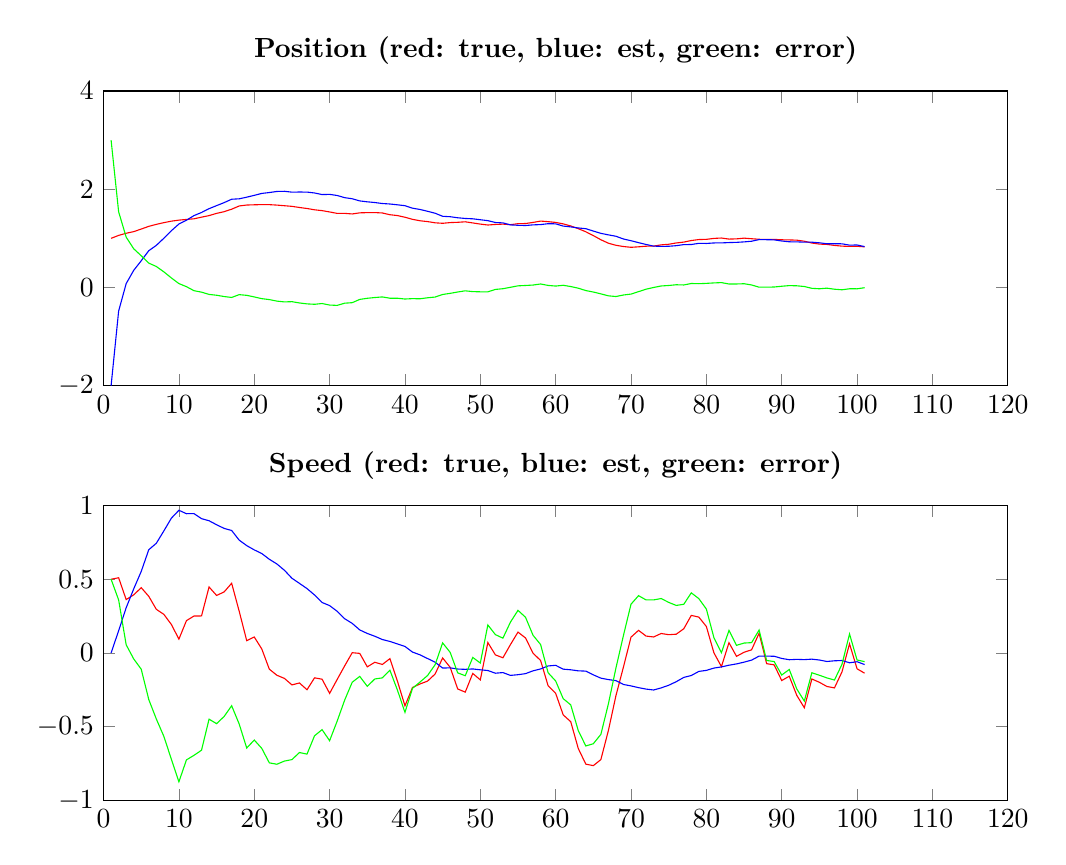
\begin{tikzpicture}

\begin{axis}[%
width=4.521in,
height=1.474in,
at={(0.758in,2.554in)},
scale only axis,
xmin=0,
xmax=120,
ymin=-2,
ymax=4,
axis background/.style={fill=white},
title style={font=\bfseries},
title={Position (red: true, blue: est, green: error)}
]
\addplot [color=red,solid,forget plot]
  table[row sep=crcr]{%
1	1\\
2	1.05983990668099\\
3	1.10346390330832\\
4	1.136507579433\\
5	1.18912895781916\\
6	1.24397462685148\\
7	1.28456854551273\\
8	1.31954138224049\\
9	1.34992741998749\\
10	1.37073649804783\\
11	1.38486850235699\\
12	1.3978243332178\\
13	1.4311473311706\\
14	1.46278246733217\\
15	1.50838008723058\\
16	1.54254615211952\\
17	1.59318044751003\\
18	1.65896544205248\\
19	1.67803532722645\\
20	1.68298834633132\\
21	1.68694794740183\\
22	1.68581663673651\\
23	1.67683405736655\\
24	1.66395772387021\\
25	1.65127695607677\\
26	1.62804435367163\\
27	1.60735783719912\\
28	1.58126362206786\\
29	1.56431201429579\\
30	1.53723520572909\\
31	1.50781381590503\\
32	1.50839123549286\\
33	1.4963741804005\\
34	1.51919793505589\\
35	1.52333166519123\\
36	1.52468683218635\\
37	1.51637114347768\\
38	1.48057359553667\\
39	1.46372228970771\\
40	1.42955240351387\\
41	1.38712089818233\\
42	1.35753772182309\\
43	1.34119136548925\\
44	1.31629106761064\\
45	1.30620390531663\\
46	1.3208224475573\\
47	1.32659150519287\\
48	1.33681816035238\\
49	1.31354480032275\\
50	1.29017710379984\\
51	1.27130488812471\\
52	1.28274163032638\\
53	1.28936786255041\\
54	1.27776528700417\\
55	1.29910382931902\\
56	1.30162952845581\\
57	1.32386878021189\\
58	1.35137595181366\\
59	1.33967545271651\\
60	1.32431972272419\\
61	1.29461757873247\\
62	1.25212150174191\\
63	1.19701575772799\\
64	1.13381170094858\\
65	1.05564719590777\\
66	0.971552033704938\\
67	0.900818712615833\\
68	0.858621727538364\\
69	0.833631779040001\\
70	0.817355391532352\\
71	0.827662399909276\\
72	0.840052271653291\\
73	0.842056734150613\\
74	0.867318547100058\\
75	0.87911876902348\\
76	0.906187125265693\\
77	0.923656835632222\\
78	0.955411413647651\\
79	0.975497922758032\\
80	0.979601030414422\\
81	0.999032180463629\\
82	1.00643909826849\\
83	0.985011899888893\\
84	0.989456728566423\\
85	1.00399871457631\\
86	0.992446740551702\\
87	0.980745454886949\\
88	0.978562141271383\\
89	0.978882636039852\\
90	0.970860355286873\\
91	0.967942514432565\\
92	0.962894684067429\\
93	0.941521485712747\\
94	0.904629715280283\\
95	0.882972240580541\\
96	0.876121284377797\\
97	0.855765520083068\\
98	0.841651502352152\\
99	0.83513961922321\\
100	0.837861904990187\\
101	0.827321948980771\\
};
\addplot [color=blue,solid,forget plot]
  table[row sep=crcr]{%
1	-2\\
2	-0.480619185889215\\
3	0.078235229335133\\
4	0.348540507512827\\
5	0.543755268824493\\
6	0.748225830137307\\
7	0.856964547893231\\
8	1.00148325009171\\
9	1.1554789333052\\
10	1.29141101271301\\
11	1.36838393286415\\
12	1.46320574143436\\
13	1.52624639463839\\
14	1.60373571960374\\
15	1.66620230676239\\
16	1.7270501933132\\
17	1.79608866550743\\
18	1.80480290322322\\
19	1.83785514583335\\
20	1.87541656916337\\
21	1.91443021815237\\
22	1.93221643955609\\
23	1.95427339559436\\
24	1.95763277814098\\
25	1.9401917246897\\
26	1.94282703945617\\
27	1.94116791411905\\
28	1.92351400697805\\
29	1.89101358619662\\
30	1.89500967157131\\
31	1.87234493492413\\
32	1.82807096133123\\
33	1.80579891481387\\
34	1.76198708976571\\
35	1.74338240457286\\
36	1.72907998532434\\
37	1.70862982535157\\
38	1.69909864456417\\
39	1.68257350385392\\
40	1.66454654985554\\
41	1.61406996762921\\
42	1.58771566815378\\
43	1.55074195552573\\
44	1.51116951149853\\
45	1.44866018583771\\
46	1.44027482642403\\
47	1.41877974388926\\
48	1.40489348794712\\
49	1.39758332481348\\
50	1.37848960080992\\
51	1.36018609697492\\
52	1.32229435958369\\
53	1.31459498020794\\
54	1.27416712763754\\
55	1.26570446534678\\
56	1.26101674168498\\
57	1.27427817187029\\
58	1.28016140150357\\
59	1.29807298342139\\
60	1.29538722273229\\
61	1.24986895072973\\
62	1.23298472762524\\
63	1.21141131801064\\
64	1.19657194263887\\
65	1.14832495955319\\
66	1.10159604322305\\
67	1.07071367222375\\
68	1.04252105558908\\
69	0.986620161911055\\
70	0.951668285417283\\
71	0.912371635584812\\
72	0.875042576374359\\
73	0.841800209394902\\
74	0.836871365764536\\
75	0.838522494120874\\
76	0.850827733243672\\
77	0.872513927489144\\
78	0.874380997726224\\
79	0.898561973559098\\
80	0.895910163734895\\
81	0.906275412305081\\
82	0.907181066822508\\
83	0.914184501227404\\
84	0.918222657480206\\
85	0.927772345766154\\
86	0.941162638085239\\
87	0.974773854721334\\
88	0.972442208959706\\
89	0.969315089186161\\
90	0.945839504979023\\
91	0.929818031059293\\
92	0.928590522290092\\
93	0.921894211261711\\
94	0.921753367793291\\
95	0.909259239184987\\
96	0.890242556382791\\
97	0.891138092519878\\
98	0.888526790621023\\
99	0.86166867356516\\
100	0.864891209327937\\
101	0.83198348079216\\
};
\addplot [color=green,solid,forget plot]
  table[row sep=crcr]{%
1	3\\
2	1.5404590925702\\
3	1.02522867397319\\
4	0.78796707192017\\
5	0.645373688994669\\
6	0.495748796714178\\
7	0.427603997619498\\
8	0.318058132148782\\
9	0.194448486682287\\
10	0.0793254853348215\\
11	0.0164845694928342\\
12	-0.0653814082165529\\
13	-0.0950990634677857\\
14	-0.140953252271576\\
15	-0.157822219531817\\
16	-0.18450404119368\\
17	-0.202908217997402\\
18	-0.145837461170742\\
19	-0.159819818606899\\
20	-0.192428222832044\\
21	-0.227482270750533\\
22	-0.24639980281958\\
23	-0.277439338227811\\
24	-0.293675054270778\\
25	-0.288914768612934\\
26	-0.31478268578454\\
27	-0.333810076919937\\
28	-0.342250384910189\\
29	-0.326701571900833\\
30	-0.357774465842222\\
31	-0.364531119019097\\
32	-0.319679725838371\\
33	-0.309424734413368\\
34	-0.242789154709819\\
35	-0.22005073938163\\
36	-0.204393153137984\\
37	-0.19225868187389\\
38	-0.218525049027504\\
39	-0.218851214146209\\
40	-0.234994146341675\\
41	-0.226949069446876\\
42	-0.230177946330686\\
43	-0.209550590036475\\
44	-0.194878443887889\\
45	-0.142456280521075\\
46	-0.11945237886673\\
47	-0.0921882386963857\\
48	-0.0680753275947368\\
49	-0.0840385244907296\\
50	-0.0883124970100808\\
51	-0.0888812088502167\\
52	-0.0395527292573117\\
53	-0.0252271176575323\\
54	0.00359815936662966\\
55	0.0333993639722425\\
56	0.0406127867708319\\
57	0.0495906083416047\\
58	0.0712145503100883\\
59	0.0416024692951209\\
60	0.0289324999919003\\
61	0.0447486280027409\\
62	0.0191367741166646\\
63	-0.0143955602826431\\
64	-0.0627602416902917\\
65	-0.0926777636454237\\
66	-0.130044009518113\\
67	-0.169894959607915\\
68	-0.183899328050714\\
69	-0.152988382871054\\
70	-0.134312893884932\\
71	-0.0847092356755358\\
72	-0.034990304721068\\
73	0.00025652475571103\\
74	0.0304471813355228\\
75	0.0405962749026062\\
76	0.0553593920220219\\
77	0.0511429081430775\\
78	0.0810304159214277\\
79	0.0769359491989341\\
80	0.0836908666795272\\
81	0.0927567681585474\\
82	0.0992580314459789\\
83	0.0708273986614893\\
84	0.0712340710862169\\
85	0.0762263688101538\\
86	0.0512841024664622\\
87	0.00597160016561538\\
88	0.00611993231167685\\
89	0.00956754685369066\\
90	0.0250208503078508\\
91	0.0381244833732715\\
92	0.034304161777337\\
93	0.019627274451036\\
94	-0.0171236525130086\\
95	-0.0262869986044459\\
96	-0.0141212720049942\\
97	-0.0353725724368107\\
98	-0.046875288268871\\
99	-0.0265290543419499\\
100	-0.02702930433775\\
101	-0.00466153181138917\\
};
\end{axis}

\begin{axis}[%
width=4.521in,
height=1.474in,
at={(0.758in,0.481in)},
scale only axis,
xmin=0,
xmax=120,
ymin=-1,
ymax=1,
axis background/.style={fill=white},
title style={font=\bfseries},
title={Speed (red: true, blue: est, green: error)}
]
\addplot [color=red,solid,forget plot]
  table[row sep=crcr]{%
1	0.5\\
2	0.510122749455856\\
3	0.362138508432862\\
4	0.394030333673167\\
5	0.442750727428276\\
6	0.383992947770346\\
7	0.296172837619113\\
8	0.261969106628911\\
9	0.19300103455154\\
10	0.093869146068027\\
11	0.219085731545019\\
12	0.250418324297629\\
13	0.251069252120361\\
14	0.447522503276475\\
15	0.390071097150626\\
16	0.413915660715479\\
17	0.472729452144836\\
18	0.282962975400368\\
19	0.083170267037612\\
20	0.108212867516337\\
21	0.0268814187418873\\
22	-0.110238998274411\\
23	-0.151341548906865\\
24	-0.172625860220022\\
25	-0.216767598100866\\
26	-0.203852811775666\\
27	-0.24958930674367\\
28	-0.168886865199559\\
29	-0.178072932343748\\
30	-0.274194999618962\\
31	-0.180153834190336\\
32	-0.0874466368741663\\
33	0.00171800319663391\\
34	-0.00307102984974266\\
35	-0.094252917530696\\
36	-0.0634350415325834\\
37	-0.0780772848268679\\
38	-0.0387497672223318\\
39	-0.190946603426072\\
40	-0.358886817261868\\
41	-0.234396516230178\\
42	-0.210226995094662\\
43	-0.191081294793758\\
44	-0.143033177077076\\
45	-0.0342625915502009\\
46	-0.0974686294933914\\
47	-0.244359439844068\\
48	-0.265822112288571\\
49	-0.139031904195587\\
50	-0.182881818556657\\
51	0.0706156502168507\\
52	-0.0131519493018552\\
53	-0.0328783282464159\\
54	0.0567170777536998\\
55	0.141367144209569\\
56	0.101613573953376\\
57	-0.00174058731661496\\
58	-0.0512753022558515\\
59	-0.222971026483284\\
60	-0.274040725150748\\
61	-0.42021400915268\\
62	-0.466460604188869\\
63	-0.648184155598903\\
64	-0.754365243085693\\
65	-0.764510678159179\\
66	-0.72349692382798\\
67	-0.525706524091631\\
68	-0.289673527597287\\
69	-0.0945486559198378\\
70	0.107280501751152\\
71	0.153097232175311\\
72	0.114417417816176\\
73	0.108432599551288\\
74	0.131985272528458\\
75	0.123830162222534\\
76	0.127124247826457\\
77	0.163977269668226\\
78	0.254703291200517\\
79	0.243181742369921\\
80	0.179483996297598\\
81	0.00109599190118512\\
82	-0.0929175004387265\\
83	0.0695374662445543\\
84	-0.0230081239063488\\
85	0.0045178160682655\\
86	0.0211306836574529\\
87	0.133958585685913\\
88	-0.072706196335933\\
89	-0.0808726111799098\\
90	-0.187333391343398\\
91	-0.158071977307917\\
92	-0.287809137434687\\
93	-0.371880899996923\\
94	-0.176643553950588\\
95	-0.199182018285258\\
96	-0.227619531771981\\
97	-0.237084130155474\\
98	-0.128373848304329\\
99	0.0619537839618582\\
100	-0.107552681779689\\
101	-0.137486715153962\\
};
\addplot [color=blue,solid,forget plot]
  table[row sep=crcr]{%
1	0\\
2	0.150418851015819\\
3	0.306765202813009\\
4	0.434392529238576\\
5	0.553079065223868\\
6	0.700325134768206\\
7	0.743844782315397\\
8	0.82769413208033\\
9	0.914309680721305\\
10	0.967852703247938\\
11	0.944654722758561\\
12	0.945056957422504\\
13	0.910979024663563\\
14	0.896864040378319\\
15	0.869824983019611\\
16	0.844930475725421\\
17	0.830785355406071\\
18	0.765220304511523\\
19	0.728196373058394\\
20	0.699099526200149\\
21	0.674318509639149\\
22	0.63549829333996\\
23	0.603771372140991\\
24	0.561014050000563\\
25	0.506777569487092\\
26	0.471842361431678\\
27	0.436736876909254\\
28	0.393074290040341\\
29	0.342332664640026\\
30	0.321089101057726\\
31	0.282770777328929\\
32	0.232166659352647\\
33	0.200498714723646\\
34	0.156085495666471\\
35	0.13229928278831\\
36	0.113153716442713\\
37	0.0910508450074005\\
38	0.078071856214844\\
39	0.0611076613255538\\
40	0.0442593607373416\\
41	0.00589070952957797\\
42	-0.0129610921248069\\
43	-0.0379524185274246\\
44	-0.0630399160613877\\
45	-0.102489566849742\\
46	-0.101180428062066\\
47	-0.109178455123845\\
48	-0.11126654967738\\
49	-0.108580475599234\\
50	-0.114379279226369\\
51	-0.119215025585091\\
52	-0.13751186310407\\
53	-0.133247350277075\\
54	-0.152348641952775\\
55	-0.1475754206695\\
56	-0.140477610335925\\
57	-0.121228128014512\\
58	-0.108536263322134\\
59	-0.0882611254163722\\
60	-0.0839332657685817\\
61	-0.11009856845617\\
62	-0.114238555449557\\
63	-0.121391126471148\\
64	-0.123293950895296\\
65	-0.148603142966406\\
66	-0.171058192004862\\
67	-0.18076492749505\\
68	-0.187892316460963\\
69	-0.214038748995957\\
70	-0.223583509542046\\
71	-0.235516500625304\\
72	-0.245222463836966\\
73	-0.251365552883065\\
74	-0.237129939495855\\
75	-0.219261981454104\\
76	-0.195147530509934\\
77	-0.166123511695742\\
78	-0.15310571179038\\
79	-0.125285984457957\\
80	-0.118328304191739\\
81	-0.102690907545341\\
82	-0.0948188672734175\\
83	-0.0832057749548945\\
84	-0.0744996410949488\\
85	-0.0625241770606531\\
86	-0.0486867716938719\\
87	-0.0215793606481226\\
88	-0.0217017318151653\\
89	-0.0223758616241452\\
90	-0.0373371887256266\\
91	-0.0459934371398537\\
92	-0.0436181068268129\\
93	-0.0452626758300939\\
94	-0.0421733043473057\\
95	-0.0480040111150597\\
96	-0.058018875977071\\
97	-0.0533007771859676\\
98	-0.0513854949403059\\
99	-0.0666861719422618\\
100	-0.0597181991635344\\
101	-0.0786936098454784\\
};
\addplot [color=green,solid,forget plot]
  table[row sep=crcr]{%
1	0.5\\
2	0.359703898440038\\
3	0.055373305619853\\
4	-0.0403621955654095\\
5	-0.110328337795591\\
6	-0.31633218699786\\
7	-0.447671944696284\\
8	-0.565725025451419\\
9	-0.721308646169765\\
10	-0.873983557179911\\
11	-0.725568991213542\\
12	-0.694638633124875\\
13	-0.659909772543201\\
14	-0.449341537101844\\
15	-0.479753885868985\\
16	-0.431014815009941\\
17	-0.358055903261235\\
18	-0.482257329111155\\
19	-0.645026106020782\\
20	-0.590886658683813\\
21	-0.647437090897262\\
22	-0.745737291614371\\
23	-0.755112921047856\\
24	-0.733639910220586\\
25	-0.723545167587957\\
26	-0.675695173207345\\
27	-0.686326183652924\\
28	-0.5619611552399\\
29	-0.520405596983774\\
30	-0.595284100676688\\
31	-0.462924611519265\\
32	-0.319613296226813\\
33	-0.198780711527013\\
34	-0.159156525516214\\
35	-0.226552200319006\\
36	-0.176588757975296\\
37	-0.169128129834268\\
38	-0.116821623437176\\
39	-0.252054264751625\\
40	-0.40314617799921\\
41	-0.240287225759756\\
42	-0.197265902969855\\
43	-0.153128876266334\\
44	-0.0799932610156882\\
45	0.0682269752995408\\
46	0.00371179856867498\\
47	-0.135180984720223\\
48	-0.154555562611191\\
49	-0.0304514285963532\\
50	-0.0685025393302877\\
51	0.189830675801941\\
52	0.124359913802215\\
53	0.100369022030659\\
54	0.209065719706475\\
55	0.288942564879069\\
56	0.242091184289302\\
57	0.119487540697897\\
58	0.0572609610662828\\
59	-0.134709901066912\\
60	-0.190107459382166\\
61	-0.31011544069651\\
62	-0.352222048739312\\
63	-0.526793029127754\\
64	-0.631071292190397\\
65	-0.615907535192773\\
66	-0.552438731823118\\
67	-0.34494159659658\\
68	-0.101781211136323\\
69	0.119490093076119\\
70	0.330864011293198\\
71	0.388613732800615\\
72	0.359639881653142\\
73	0.359798152434353\\
74	0.369115212024314\\
75	0.343092143676637\\
76	0.322271778336391\\
77	0.330100781363969\\
78	0.407809002990897\\
79	0.368467726827878\\
80	0.297812300489337\\
81	0.103786899446526\\
82	0.001901366834691\\
83	0.152743241199449\\
84	0.0514915171885999\\
85	0.0670419931289186\\
86	0.0698174553513249\\
87	0.155537946334036\\
88	-0.0510044645207677\\
89	-0.0584967495557646\\
90	-0.149996202617772\\
91	-0.112078540168064\\
92	-0.244191030607874\\
93	-0.326618224166829\\
94	-0.134470249603283\\
95	-0.151178007170198\\
96	-0.16960065579491\\
97	-0.183783352969506\\
98	-0.0769883533640228\\
99	0.12863995590412\\
100	-0.0478344826161542\\
101	-0.0587931053084836\\
};
\end{axis}
\end{tikzpicture}%}
	\scalebox{0.5}{% This file was created by matlab2tikz.
%
%The latest updates can be retrieved from
%  http://www.mathworks.com/matlabcentral/fileexchange/22022-matlab2tikz-matlab2tikz
%where you can also make suggestions and rate matlab2tikz.
%
\definecolor{mycolor1}{rgb}{0.00000,0.44700,0.74100}%
%
\begin{tikzpicture}

\begin{axis}[%
width=4.521in,
height=1.474in,
at={(0.758in,2.554in)},
scale only axis,
xmin=0,
xmax=120,
ymin=0.2,
ymax=1,
axis background/.style={fill=white},
title style={font=\bfseries},
title={sqrt(P(1,1))}
]
\addplot [color=mycolor1,solid,forget plot]
  table[row sep=crcr]{%
1	1\\
2	0.708881028678478\\
3	0.58586175928378\\
4	0.521254311048763\\
5	0.486794691325772\\
6	0.470040399427915\\
7	0.463498977656542\\
8	0.462124661214206\\
9	0.462628568230894\\
10	0.463091000028693\\
11	0.462578929934614\\
12	0.460789369830808\\
13	0.457769321178245\\
14	0.453726793238945\\
15	0.448919029709919\\
16	0.443594721585136\\
17	0.43796919635921\\
18	0.432217572509656\\
19	0.426476555744323\\
20	0.420849656685714\\
21	0.415413175760977\\
22	0.410221759021837\\
23	0.405313093692933\\
24	0.400711681126271\\
25	0.396431782078416\\
26	0.392479680446666\\
27	0.388855413713747\\
28	0.385554100452377\\
29	0.38256697138236\\
30	0.379882186935215\\
31	0.377485503521791\\
32	0.375360833401762\\
33	0.373490729155274\\
34	0.371856812921742\\
35	0.370440162400502\\
36	0.369221659714697\\
37	0.368182305262376\\
38	0.367303496280146\\
39	0.366567268705672\\
40	0.365956500743349\\
41	0.365455077030061\\
42	0.365048013209472\\
43	0.364721541833212\\
44	0.364463161636195\\
45	0.364261653246837\\
46	0.364107065201664\\
47	0.363990674689607\\
48	0.363904927741551\\
49	0.363843363620072\\
50	0.363800527986631\\
51	0.363771879073772\\
52	0.363753690617198\\
53	0.363742954755109\\
54	0.363737287522734\\
55	0.36373483899458\\
56	0.363734209582901\\
57	0.363734373507821\\
58	0.363734610024323\\
59	0.3637344426294\\
60	0.36373358617987\\
61	0.363731901624289\\
62	0.363729357885528\\
63	0.363726000316698\\
64	0.363721925084273\\
65	0.363717258800666\\
66	0.363712142726427\\
67	0.363706720882865\\
68	0.363701131453026\\
69	0.363695500897397\\
70	0.363689940266046\\
71	0.363684543247649\\
72	0.36367938555511\\
73	0.363674525305278\\
74	0.363670004104914\\
75	0.3636658486056\\
76	0.363662072336046\\
77	0.363658677660832\\
78	0.363655657750089\\
79	0.363652998474903\\
80	0.363650680168758\\
81	0.363648679216317\\
82	0.363646969447819\\
83	0.363645523330663\\
84	0.363644312959956\\
85	0.363643310857225\\
86	0.363642490591693\\
87	0.363641827241805\\
88	0.363641297716462\\
89	0.363640880956021\\
90	0.363640558032775\\
91	0.363640312169665\\
92	0.363640128694501\\
93	0.363639994945256\\
94	0.363639900140109\\
95	0.363639835223976\\
96	0.36363979270139\\
97	0.363639766463784\\
98	0.363639751617604\\
99	0.363639744318171\\
100	0.363639741612921\\
101	0.363639741296508\\
};
\end{axis}

\begin{axis}[%
width=4.521in,
height=1.474in,
at={(0.758in,0.481in)},
scale only axis,
xmin=0,
xmax=120,
ymin=0,
ymax=1.5,
axis background/.style={fill=white},
title style={font=\bfseries},
title={sqrt(P(2,2))}
]
\addplot [color=mycolor1,solid,forget plot]
  table[row sep=crcr]{%
1	1\\
2	1.00250941298733\\
3	1.00009916349816\\
4	0.990678620316673\\
5	0.972852099354142\\
6	0.946247399992162\\
7	0.911633199786077\\
8	0.87073738854666\\
9	0.825831969387544\\
10	0.7792592572927\\
11	0.733064415069595\\
12	0.688806241346389\\
13	0.647526560532727\\
14	0.609816620728331\\
15	0.575921333795093\\
16	0.545843260633164\\
17	0.51942887576768\\
18	0.496432977755596\\
19	0.476563543483088\\
20	0.459511390396938\\
21	0.444968941945965\\
22	0.43264155348836\\
23	0.422253916076102\\
24	0.413553269025525\\
25	0.406310573419438\\
26	0.400320402145973\\
27	0.395400041147584\\
28	0.391388127799164\\
29	0.388143042888205\\
30	0.385541200331776\\
31	0.383475329629096\\
32	0.381852811823059\\
33	0.380594105579436\\
34	0.379631282991119\\
35	0.378906683023493\\
36	0.378371682828884\\
37	0.377985582466194\\
38	0.37771459605043\\
39	0.377530941357755\\
40	0.377412019886954\\
41	0.377339679910532\\
42	0.377299555830139\\
43	0.377280477970628\\
44	0.37727394767449\\
45	0.377273673128059\\
46	0.377275161744839\\
47	0.377275365164202\\
48	0.377272373029489\\
49	0.377265151730339\\
50	0.377253324272486\\
51	0.377236987411353\\
52	0.377216562182701\\
53	0.377192674003533\\
54	0.377166058609802\\
55	0.377137490246327\\
56	0.377107728724762\\
57	0.37707748220906\\
58	0.37704738286392\\
59	0.377017972798244\\
60	0.376989698041319\\
61	0.376962908593669\\
62	0.376937862888601\\
63	0.3769147352775\\
64	0.376893625406802\\
65	0.376874568584199\\
66	0.376857546434282\\
67	0.376842497319225\\
68	0.376829326148931\\
69	0.376817913328806\\
70	0.376808122693979\\
71	0.37679980835867\\
72	0.37679282047103\\
73	0.376787009909586\\
74	0.37678223198994\\
75	0.376778349271742\\
76	0.376775233568409\\
77	0.376772767267385\\
78	0.376770844068571\\
79	0.376769369244407\\
80	0.376768259517996\\
81	0.376767442646815\\
82	0.376766856789549\\
83	0.376766449723257\\
84	0.376766177967738\\
85	0.376766005864103\\
86	0.376765904645376\\
87	0.37676585152858\\
88	0.376765828850407\\
89	0.376765823262098\\
90	0.376765824993778\\
91	0.376765827193905\\
92	0.376765825345882\\
93	0.376765816760999\\
94	0.376765800144682\\
95	0.376765775231484\\
96	0.376765742483186\\
97	0.376765702843738\\
98	0.376765657544534\\
99	0.376765607953467\\
100	0.376765555461446\\
101	0.376765501400414\\
};
\end{axis}
\end{tikzpicture}%}
	\scalebox{0.5}{% This file was created by matlab2tikz.
%
%The latest updates can be retrieved from
%  http://www.mathworks.com/matlabcentral/fileexchange/22022-matlab2tikz-matlab2tikz
%where you can also make suggestions and rate matlab2tikz.
%
\definecolor{mycolor1}{rgb}{0.00000,0.44700,0.74100}%
%
\begin{tikzpicture}

\begin{axis}[%
width=4.521in,
height=1.474in,
at={(0.758in,2.554in)},
scale only axis,
xmin=0,
xmax=100,
ymin=0,
ymax=0.6,
axis background/.style={fill=white},
title style={font=\bfseries},
title={K(1)}
]
\addplot [color=mycolor1,solid,forget plot]
  table[row sep=crcr]{%
1	0.502512312820258\\
2	0.343234000991086\\
3	0.27170605678692\\
4	0.236969071502954\\
5	0.220937977094354\\
6	0.21483130228866\\
7	0.213559202502345\\
8	0.214025192143366\\
9	0.214453274307575\\
10	0.213979266419452\\
11	0.212326843349073\\
12	0.209552751411991\\
13	0.205868002902897\\
14	0.201528295235695\\
15	0.196776277018195\\
16	0.191817016959532\\
17	0.186812029986139\\
18	0.181882252599541\\
19	0.177114433532484\\
20	0.17256810659582\\
21	0.16828189157497\\
22	0.164278703918936\\
23	0.160569851391043\\
24	0.157158157841869\\
25	0.154040299563517\\
26	0.151208532774489\\
27	0.148651964375642\\
28	0.146357487592672\\
29	0.144310475950682\\
30	0.1424953053691\\
31	0.140895755252065\\
32	0.139495324764938\\
33	0.138277489316315\\
34	0.13722591391931\\
35	0.136324634002475\\
36	0.135558209908317\\
37	0.134911858379619\\
38	0.134371562486336\\
39	0.133924160436317\\
40	0.133557413327048\\
41	0.133260051948183\\
42	0.133021803077196\\
43	0.132833396189851\\
44	0.132686552026119\\
45	0.132573954929769\\
46	0.132489211260995\\
47	0.132426796434583\\
48	0.132381993250368\\
49	0.132350824163352\\
50	0.132329980004863\\
51	0.132316747437632\\
52	0.132308937133977\\
53	0.132304814334396\\
54	0.132303033098413\\
55	0.132302575220898\\
56	0.132302694471127\\
57	0.132302866529547\\
58	0.13230274475492\\
59	0.132302121715269\\
60	0.132300896259221\\
61	0.132299045787819\\
62	0.132296603306383\\
63	0.13229363878701\\
64	0.132290244349471\\
65	0.132286522766649\\
66	0.132282578815366\\
67	0.132278513020212\\
68	0.132274417373008\\
69	0.13227037265072\\
70	0.132266446997251\\
71	0.132262695477742\\
72	0.132259160356019\\
73	0.132255871885668\\
74	0.132252849442031\\
75	0.132250102855747\\
76	0.132247633838025\\
77	0.132245437413649\\
78	0.132243503299788\\
79	0.1322418171872\\
80	0.132240361895772\\
81	0.132239118388583\\
82	0.132238066638431\\
83	0.132237186348118\\
84	0.132236457531204\\
85	0.13223586096373\\
86	0.132235378519759\\
87	0.132234993404913\\
88	0.132234690302471\\
89	0.132234455446388\\
90	0.132234276634852\\
91	0.132234143196953\\
92	0.132234045923786\\
93	0.132233976973908\\
94	0.132233929761721\\
95	0.13223389883591\\
96	0.132233879753835\\
97	0.132233868956513\\
98	0.132233863647785\\
99	0.132233861680312\\
100	0.132233861450191\\
};
\end{axis}

\begin{axis}[%
width=4.521in,
height=1.474in,
at={(0.758in,0.481in)},
scale only axis,
xmin=0,
xmax=100,
ymin=0,
ymax=0.3,
axis background/.style={fill=white},
title style={font=\bfseries},
title={K(2)}
]
\addplot [color=mycolor1,solid,forget plot]
  table[row sep=crcr]{%
1	0.0497487687179742\\
2	0.0986799326885588\\
3	0.144711836366239\\
4	0.185306829350047\\
5	0.218099153477312\\
6	0.241547388379646\\
7	0.255321856481653\\
8	0.260267868008078\\
9	0.258026735794226\\
10	0.250545079408666\\
11	0.239675884368301\\
12	0.226954232252985\\
13	0.213528829563192\\
14	0.200189999751546\\
15	0.18743911370089\\
16	0.175564499041413\\
17	0.164707266955031\\
18	0.154912098430594\\
19	0.146163715281028\\
20	0.13841180351291\\
21	0.131587402316179\\
22	0.125613318141593\\
23	0.12041050900736\\
24	0.11590182793473\\
25	0.112014079004462\\
26	0.10867902302581\\
27	0.105833749482166\\
28	0.103420682169789\\
29	0.101387386687772\\
30	0.0996862828139561\\
31	0.0982743225748214\\
32	0.0971126677911808\\
33	0.0961663838934769\\
34	0.0954041564274834\\
35	0.0947980306525134\\
36	0.0943231714717202\\
37	0.0939576396246447\\
38	0.0936821799329512\\
39	0.093480017947645\\
40	0.0933366622665551\\
41	0.0932397108393266\\
42	0.0931786605912042\\
43	0.0931447205707074\\
44	0.0931306294994679\\
45	0.0931304790507756\\
46	0.0931395444105033\\
47	0.0931541237038563\\
48	0.0931713877403522\\
49	0.0931892412802624\\
50	0.0932061967017745\\
51	0.0932212605892751\\
52	0.0932338334031415\\
53	0.0932436220563872\\
54	0.0932505649316599\\
55	0.0932547686342218\\
56	0.0932564555970732\\
57	0.0932559215326571\\
58	0.0932535016572847\\
59	0.0932495445928505\\
60	0.0932443928675947\\
61	0.0932383689852962\\
62	0.0932317661022734\\
63	0.0932248424366229\\
64	0.093217818627859\\
65	0.0932108773622754\\
66	0.0932041646757389\\
67	0.0931977924380897\\
68	0.0931918416096156\\
69	0.093186365938713\\
70	0.0931813958400248\\
71	0.0931769422537485\\
72	0.0931730003395\\
73	0.0931695529024912\\
74	0.0931665734863771\\
75	0.0931640290966729\\
76	0.0931618825418705\\
77	0.0931600943971179\\
78	0.0931586246083173\\
79	0.0931574337635131\\
80	0.0931564840641678\\
81	0.0931557400319951\\
82	0.093155168988002\\
83	0.0931547413397799\\
84	0.0931544307113071\\
85	0.0931542139469325\\
86	0.0931540710181146\\
87	0.093153984858116\\
88	0.0931539411463996\\
89	0.0931539280610856\\
90	0.0931539360146048\\
91	0.0931539573847096\\
92	0.093153986250314\\
93	0.0931540181392632\\
94	0.0931540497930805\\
95	0.0931540789520061\\
96	0.0931541041622056\\
97	0.093154124605868\\
98	0.0931541399540092\\
99	0.0931541502411086\\
100	0.0931541557602137\\
};
\end{axis}
\end{tikzpicture}%}

	\caption{$Q \times 100,R$ default.}
	\label{fig:q3:Qx100}
\end{figure}

\begin{figure}[H]
	\scalebox{0.5}{% This file was created by matlab2tikz.
%
%The latest updates can be retrieved from
%  http://www.mathworks.com/matlabcentral/fileexchange/22022-matlab2tikz-matlab2tikz
%where you can also make suggestions and rate matlab2tikz.
%
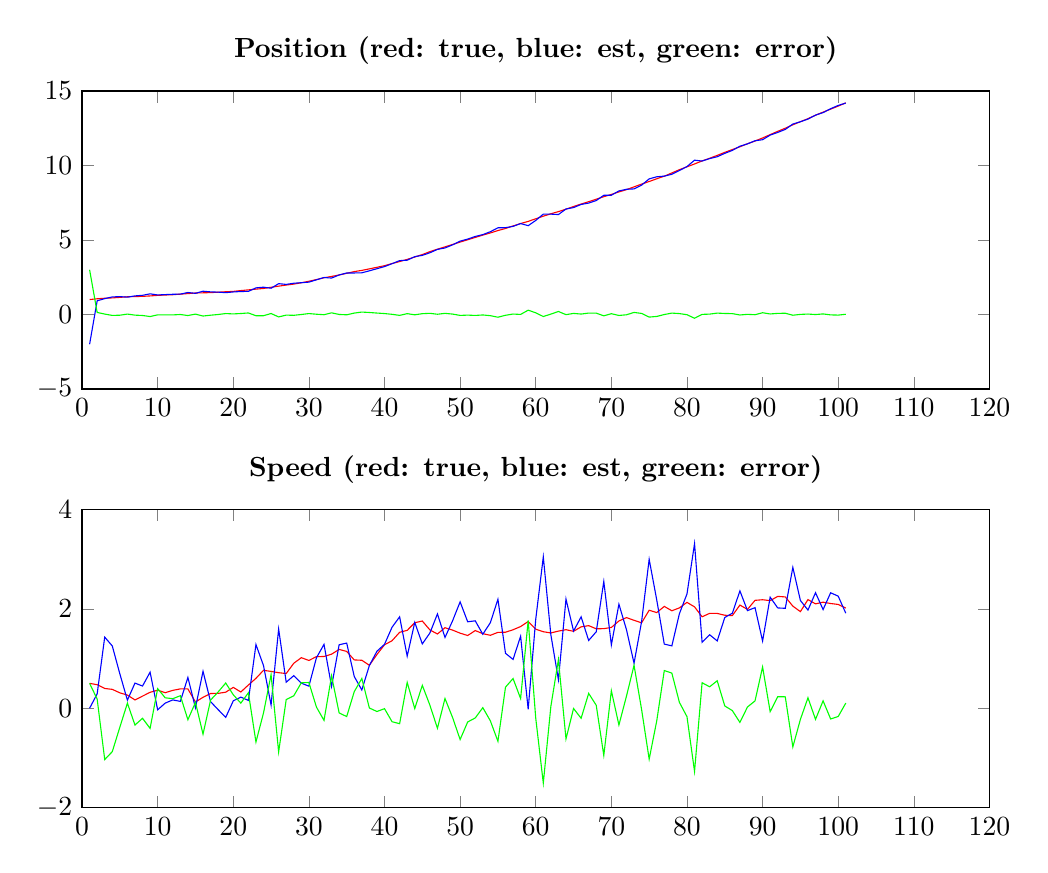
\begin{tikzpicture}

\begin{axis}[%
width=4.537in,
height=1.49in,
at={(0.761in,2.579in)},
scale only axis,
xmin=0,
xmax=120,
ymin=-5,
ymax=15,
axis background/.style={fill=white},
title style={font=\bfseries},
title={Position (red: true, blue: est, green: error)}
]
\addplot [color=red,solid,forget plot]
  table[row sep=crcr]{%
1	1\\
2	1.05183431871122\\
3	1.08766257573903\\
4	1.11095775832048\\
5	1.14515392287417\\
6	1.18714727663149\\
7	1.1993055450085\\
8	1.21490831353166\\
9	1.24305107969992\\
10	1.2808707790602\\
11	1.30475933653124\\
12	1.32490677367331\\
13	1.36185050215931\\
14	1.40058781473535\\
15	1.43855377224548\\
16	1.45297229122178\\
17	1.46561369967028\\
18	1.4931946909479\\
19	1.52451040009455\\
20	1.54634837960185\\
21	1.60243938428865\\
22	1.64935591835372\\
23	1.6982008966854\\
24	1.74554291872294\\
25	1.82419111113177\\
26	1.89926025642081\\
27	1.97271249531131\\
28	2.0364027139049\\
29	2.12768725440426\\
30	2.22847805045342\\
31	2.34072565671523\\
32	2.46165627661344\\
33	2.55158065161113\\
34	2.65057395430947\\
35	2.76022103643888\\
36	2.87680991710737\\
37	2.95635500091804\\
38	3.05992311710618\\
39	3.16432334008696\\
40	3.27207130969576\\
41	3.41699485305326\\
42	3.54941018794628\\
43	3.69596062969527\\
44	3.85425542897659\\
45	4.0187828837623\\
46	4.21457999884664\\
47	4.37996150423643\\
48	4.53597041752025\\
49	4.69631218957155\\
50	4.85733088233153\\
51	5.01273551390677\\
52	5.16899214839812\\
53	5.32468760202437\\
54	5.47017069160255\\
55	5.63146452953163\\
56	5.76895392991393\\
57	5.9381079728163\\
58	6.10167165018778\\
59	6.24584283225995\\
60	6.4216144838552\\
61	6.59476349915201\\
62	6.75657629570879\\
63	6.90318141294712\\
64	7.06464112070531\\
65	7.24321992362552\\
66	7.40988255931832\\
67	7.56775997554495\\
68	7.73472221519327\\
69	7.90432379796964\\
70	8.05368559300071\\
71	8.22250095749648\\
72	8.37702566311811\\
73	8.56286421520239\\
74	8.74881383915631\\
75	8.9224485128086\\
76	9.10658043960519\\
77	9.27842736391258\\
78	9.49743775373254\\
79	9.71680041859413\\
80	9.90856954503785\\
81	10.0990618880692\\
82	10.3030436421989\\
83	10.4829486446255\\
84	10.6750142210062\\
85	10.8776135028085\\
86	11.066781897045\\
87	11.2546019281457\\
88	11.4557302936412\\
89	11.6389543513933\\
90	11.8445618367076\\
91	12.068832838593\\
92	12.2890841448102\\
93	12.4995836711032\\
94	12.7279645558646\\
95	12.9366127192525\\
96	13.1394599551468\\
97	13.3720128359979\\
98	13.5800645714585\\
99	13.7793799029902\\
100	13.9851400019251\\
101	14.1995103386685\\
};
\addplot [color=blue,solid,forget plot]
  table[row sep=crcr]{%
1	-2\\
2	0.916066733168057\\
3	1.06149026016169\\
4	1.17615515182326\\
5	1.19586461676306\\
6	1.16228928427234\\
7	1.24543403104984\\
8	1.28441768707234\\
9	1.38357929718366\\
10	1.30858144448068\\
11	1.33165306919499\\
12	1.35445754913839\\
13	1.36547049232025\\
14	1.47317522844148\\
15	1.41581719626386\\
16	1.55992116405812\\
17	1.51521486855463\\
18	1.49716197839676\\
19	1.46393996210832\\
20	1.51032001201185\\
21	1.53984374037413\\
22	1.5492657573017\\
23	1.78399826980997\\
24	1.82961076368246\\
25	1.76105000840932\\
26	2.06565598099904\\
27	2.01655268837289\\
28	2.09455858052716\\
29	2.13074237647112\\
30	2.16947346089955\\
31	2.32527866541992\\
32	2.47930399947658\\
33	2.4426571332626\\
34	2.65018417510923\\
35	2.78446786400598\\
36	2.78462903327106\\
37	2.79569206452645\\
38	2.92846575176697\\
39	3.07030558400318\\
40	3.21216055076807\\
41	3.40798555843957\\
42	3.61171811861993\\
43	3.64157648648385\\
44	3.87875192465948\\
45	3.96727231551025\\
46	4.13939365009866\\
47	4.3655455875493\\
48	4.46322859585974\\
49	4.67078360973107\\
50	4.92119189812985\\
51	5.05726043651895\\
52	5.23501227036002\\
53	5.35847654848248\\
54	5.55282187883574\\
55	5.81689488398057\\
56	5.82441729941015\\
57	5.91094213880973\\
58	6.10020223689038\\
59	5.95877457845053\\
60	6.30959710437354\\
61	6.73343863802736\\
62	6.73250209276249\\
63	6.70428204199718\\
64	7.07796501900789\\
65	7.17235775397954\\
66	7.38350677145024\\
67	7.47487056601743\\
68	7.64540178298089\\
69	7.99666192066943\\
70	8.00302632474825\\
71	8.29022066150235\\
72	8.39959792236028\\
73	8.42625354535809\\
74	8.68038197536455\\
75	9.09892553505244\\
76	9.2397875870097\\
77	9.28451022057487\\
78	9.40669222939052\\
79	9.65846288762915\\
80	9.92604424341327\\
81	10.3533089887473\\
82	10.298043894621\\
83	10.4602866876087\\
84	10.5841865710673\\
85	10.8114072086954\\
86	11.0109629815631\\
87	11.2897678499265\\
88	11.4486194392053\\
89	11.6568407476023\\
90	11.7285634433557\\
91	12.0357775252299\\
92	12.2172434065409\\
93	12.4176341249346\\
94	12.7790767240615\\
95	12.9329771616611\\
96	13.1124668361983\\
97	13.3779981484515\\
98	13.5445558776033\\
99	13.8090692049593\\
100	14.0282270665223\\
101	14.1871374967737\\
};
\addplot [color=green,solid,forget plot]
  table[row sep=crcr]{%
1	3\\
2	0.135767585543163\\
3	0.0261723155773406\\
4	-0.0651973935027783\\
5	-0.0507106938888868\\
6	0.0248579923591543\\
7	-0.0461284860413376\\
8	-0.0695093735406809\\
9	-0.140528217483735\\
10	-0.0277106654204757\\
11	-0.0268937326637495\\
12	-0.0295507754650783\\
13	-0.00361999016094017\\
14	-0.0725874137061335\\
15	0.0227365759816243\\
16	-0.106948872836339\\
17	-0.0496011688843454\\
18	-0.00396728744885766\\
19	0.0605704379862222\\
20	0.0360283675899944\\
21	0.062595643914523\\
22	0.100090161052023\\
23	-0.0857973731245691\\
24	-0.0840678449595271\\
25	0.0631411027224464\\
26	-0.166395724578229\\
27	-0.0438401930615782\\
28	-0.0581558666222572\\
29	-0.00305512206685954\\
30	0.0590045895538744\\
31	0.0154469912953128\\
32	-0.0176477228631451\\
33	0.108923518348524\\
34	0.000389779200236529\\
35	-0.0242468275670995\\
36	0.0921808838363076\\
37	0.160662936391593\\
38	0.131457365339219\\
39	0.0940177560837765\\
40	0.0599107589276926\\
41	0.00900929461368927\\
42	-0.0623079306736569\\
43	0.0543841432114163\\
44	-0.0244964956828868\\
45	0.0515105682520587\\
46	0.0751863487479811\\
47	0.014415916687132\\
48	0.0727418216605011\\
49	0.0255285798404818\\
50	-0.0638610157983122\\
51	-0.0445249226121858\\
52	-0.066020121961893\\
53	-0.0337889464581096\\
54	-0.0826511872331954\\
55	-0.185430354448942\\
56	-0.0554633694962172\\
57	0.0271658340065679\\
58	0.00146941329739292\\
59	0.287068253809414\\
60	0.112017379481656\\
61	-0.138675138875351\\
62	0.0240742029462977\\
63	0.198899370949944\\
64	-0.0133238983025752\\
65	0.0708621696459799\\
66	0.0263757878680817\\
67	0.0928894095275217\\
68	0.0893204322123715\\
69	-0.0923381226997835\\
70	0.0506592682524598\\
71	-0.0677197040058761\\
72	-0.0225722592421675\\
73	0.136610669844302\\
74	0.0684318637917674\\
75	-0.176477022243837\\
76	-0.133207147404505\\
77	-0.00608285666228348\\
78	0.0907455243420205\\
79	0.0583375309649856\\
80	-0.0174746983754215\\
81	-0.254247100678167\\
82	0.00499974757790156\\
83	0.0226619570168474\\
84	0.0908276499389\\
85	0.0662062941130781\\
86	0.055818915481888\\
87	-0.0351659217808145\\
88	0.00711085443591664\\
89	-0.0178863962089153\\
90	0.115998393351951\\
91	0.0330553133630787\\
92	0.0718407382692927\\
93	0.0819495461686035\\
94	-0.0511121681969424\\
95	0.00363555759138556\\
96	0.0269931189485249\\
97	-0.00598531245356604\\
98	0.0355086938551779\\
99	-0.029689301969082\\
100	-0.0430870645972377\\
101	0.0123728418947664\\
};
\end{axis}

\begin{axis}[%
width=4.537in,
height=1.49in,
at={(0.761in,0.486in)},
scale only axis,
xmin=0,
xmax=120,
ymin=-2,
ymax=4,
axis background/.style={fill=white},
title style={font=\bfseries},
title={Speed (red: true, blue: est, green: error)}
]
\addplot [color=red,solid,forget plot]
  table[row sep=crcr]{%
1	0.5\\
2	0.474026770329077\\
3	0.397828134350594\\
4	0.379629072623643\\
5	0.309825545665041\\
6	0.265164748561258\\
7	0.167393137706137\\
8	0.243849292805115\\
9	0.32051457422243\\
10	0.363111875834507\\
11	0.312616708686993\\
12	0.359435141097909\\
13	0.389578599180006\\
14	0.388702806304801\\
15	0.124588227555646\\
16	0.220560448280626\\
17	0.296647258720324\\
18	0.299121178644418\\
19	0.322879796911794\\
20	0.41945646109844\\
21	0.327037795505751\\
22	0.467798560176717\\
23	0.601909690766966\\
24	0.763747279861292\\
25	0.741189666789234\\
26	0.715516416699725\\
27	0.698176017297208\\
28	0.905356011713941\\
29	1.017682731033\\
30	0.96202074165837\\
31	1.03887028507247\\
32	1.04123367060628\\
33	1.08876102630063\\
34	1.18369897856383\\
35	1.14388626141138\\
36	0.972742203156134\\
37	0.965493038938867\\
38	0.864946239463521\\
39	1.08118465506114\\
40	1.27748505430036\\
41	1.35946588245167\\
42	1.52878081115629\\
43	1.56805344989227\\
44	1.72124125943825\\
45	1.75603967350872\\
46	1.57666972010215\\
47	1.49463561048839\\
48	1.62040548713319\\
49	1.57323823837288\\
50	1.5113767105189\\
51	1.46414363499895\\
52	1.56345437868998\\
53	1.50144451528009\\
54	1.46823582724137\\
55	1.52781903799023\\
56	1.53008779551039\\
57	1.58021511270516\\
58	1.64445945823517\\
59	1.74676755243568\\
60	1.59163440489658\\
61	1.54028690921365\\
62	1.51564139819927\\
63	1.5530908768144\\
64	1.58103737499702\\
65	1.54866293987997\\
66	1.63812121519869\\
67	1.66301293503145\\
68	1.59922047559689\\
69	1.60225537658194\\
70	1.62628188048906\\
71	1.75678530127807\\
72	1.82495818801004\\
73	1.77021691169125\\
74	1.71951135669796\\
75	1.97318535971185\\
76	1.92577188630782\\
77	2.05017449830616\\
78	1.96218635876275\\
79	2.02098767917213\\
80	2.13132275256115\\
81	2.04099417089267\\
82	1.84104026401236\\
83	1.9104980996407\\
84	1.90871225349661\\
85	1.87218498516786\\
86	1.86549033490268\\
87	2.0767921822962\\
88	1.98983930958199\\
89	2.17241443238454\\
90	2.18447541424904\\
91	2.16632886756654\\
92	2.25170032979702\\
93	2.24131070605685\\
94	2.05584226881415\\
95	1.9446860935589\\
96	2.18733262461602\\
97	2.10126707839598\\
98	2.13529278191389\\
99	2.1082153665566\\
100	2.08978054330625\\
101	2.01642122152166\\
};
\addplot [color=blue,solid,forget plot]
  table[row sep=crcr]{%
1	0\\
2	0.288690895274533\\
3	1.43127618131369\\
4	1.254096796099\\
5	0.692181107008092\\
6	0.16265046999728\\
7	0.506089292849124\\
8	0.446388097016936\\
9	0.726405704104758\\
10	-0.0318362758186603\\
11	0.103005150136657\\
12	0.167222806033187\\
13	0.1379008906022\\
14	0.620226088122554\\
15	0.00711308502710972\\
16	0.743546591012806\\
17	0.132075427435495\\
18	-0.0284713558757833\\
19	-0.184470135717913\\
20	0.148467560481938\\
21	0.223845297610165\\
22	0.157272651428666\\
23	1.28203596175925\\
24	0.857866026343654\\
25	0.0651715712597963\\
26	1.59609088432131\\
27	0.524189496340381\\
28	0.655598467205244\\
29	0.504729460579308\\
30	0.444425813453392\\
31	1.01636002140623\\
32	1.28542023389316\\
33	0.437046030374497\\
34	1.27840243985818\\
35	1.31149457128027\\
36	0.638767218654607\\
37	0.367527592225722\\
38	0.860670191125552\\
39	1.14710722708729\\
40	1.28651415988139\\
41	1.63150311451825\\
42	1.83992471614504\\
43	1.04832548802203\\
44	1.7280097793395\\
45	1.29516301760817\\
46	1.51397319835216\\
47	1.89789665307803\\
48	1.42485689866989\\
49	1.75903879224789\\
50	2.1416772308463\\
51	1.7405768071396\\
52	1.75954917401251\\
53	1.48996866894786\\
54	1.7228685126345\\
55	2.19426223275793\\
56	1.10597037102416\\
57	0.982340800039517\\
58	1.44983062802221\\
59	-0.0211125334487503\\
60	1.79147858330424\\
61	3.0481720716319\\
62	1.47788730967281\\
63	0.573944493825585\\
64	2.19833356958621\\
65	1.55409782211769\\
66	1.84036240947035\\
67	1.36441688386968\\
68	1.53949328715485\\
69	2.55283868108618\\
70	1.27444246119685\\
71	2.09488417631147\\
72	1.58073505227064\\
73	0.905801396429118\\
74	1.74574983913145\\
75	2.99871937390792\\
76	2.18207919168846\\
77	1.29109650302408\\
78	1.25551764331565\\
79	1.90375042606857\\
80	2.30026525588353\\
81	3.3132378473336\\
82	1.32780146005986\\
83	1.47911520595794\\
84	1.35579666086493\\
85	1.82644475607243\\
86	1.91329750009356\\
87	2.36255067952669\\
88	1.96502325061021\\
89	2.02520939979726\\
90	1.35345806994931\\
91	2.23613614328115\\
92	2.01967455488731\\
93	2.01157677615436\\
94	2.83476526631203\\
95	2.16929065968883\\
96	1.97701008947414\\
97	2.32537177214935\\
98	1.98651567938433\\
99	2.32476734886661\\
100	2.25636451272642\\
101	1.91367418365018\\
};
\addplot [color=green,solid,forget plot]
  table[row sep=crcr]{%
1	0.5\\
2	0.185335875054544\\
3	-1.0334480469631\\
4	-0.874467723475358\\
5	-0.382355561343051\\
6	0.102514278563978\\
7	-0.338696155142987\\
8	-0.202538804211821\\
9	-0.405891129882328\\
10	0.394948151653167\\
11	0.209611558550336\\
12	0.192212335064723\\
13	0.251677708577806\\
14	-0.231523281817754\\
15	0.117475142528536\\
16	-0.52298614273218\\
17	0.164571831284829\\
18	0.327592534520201\\
19	0.507349932629707\\
20	0.270988900616503\\
21	0.103192497895586\\
22	0.310525908748052\\
23	-0.680126270992282\\
24	-0.0941187464823628\\
25	0.676018095529438\\
26	-0.880574467621583\\
27	0.173986520956827\\
28	0.249757544508697\\
29	0.512953270453696\\
30	0.517594928204978\\
31	0.022510263666238\\
32	-0.244186563286879\\
33	0.651714995926134\\
34	-0.0947034612943525\\
35	-0.167608309868887\\
36	0.333974984501526\\
37	0.597965446713145\\
38	0.00427604833796869\\
39	-0.0659225720261478\\
40	-0.00902910558102699\\
41	-0.272037232066584\\
42	-0.311143904988755\\
43	0.519727961870241\\
44	-0.00676851990125638\\
45	0.460876655900553\\
46	0.0626965217499884\\
47	-0.403261042589638\\
48	0.195548588463304\\
49	-0.185800553875014\\
50	-0.630300520327393\\
51	-0.276433172140657\\
52	-0.19609479532253\\
53	0.0114758463322344\\
54	-0.254632685393131\\
55	-0.666443194767701\\
56	0.424117424486232\\
57	0.597874312665639\\
58	0.194628830212958\\
59	1.76788008588443\\
60	-0.199844178407655\\
61	-1.50788516241825\\
62	0.0377540885264529\\
63	0.979146382988812\\
64	-0.617296194589193\\
65	-0.00543488223771282\\
66	-0.202241194271654\\
67	0.29859605116177\\
68	0.0597271884420345\\
69	-0.950583304504238\\
70	0.351839419292213\\
71	-0.338098875033392\\
72	0.244223135739397\\
73	0.864415515262132\\
74	-0.0262384824334885\\
75	-1.02553401419607\\
76	-0.256307305380632\\
77	0.759077995282083\\
78	0.706668715447097\\
79	0.117237253103555\\
80	-0.168942503322375\\
81	-1.27224367644093\\
82	0.513238803952502\\
83	0.43138289368276\\
84	0.552915592631678\\
85	0.0457402290954283\\
86	-0.0478071651908871\\
87	-0.285758497230486\\
88	0.0248160589717799\\
89	0.147205032587278\\
90	0.831017344299733\\
91	-0.0698072757146115\\
92	0.232025774909713\\
93	0.229733929902491\\
94	-0.778922997497878\\
95	-0.22460456612993\\
96	0.210322535141875\\
97	-0.224104693753361\\
98	0.148777102529555\\
99	-0.216551982310011\\
100	-0.166583969420169\\
101	0.102747037871475\\
};
\end{axis}
\end{tikzpicture}%}
	\scalebox{0.5}{% This file was created by matlab2tikz.
%
%The latest updates can be retrieved from
%  http://www.mathworks.com/matlabcentral/fileexchange/22022-matlab2tikz-matlab2tikz
%where you can also make suggestions and rate matlab2tikz.
%
\definecolor{mycolor1}{rgb}{0.00000,0.44700,0.74100}%
%
\begin{tikzpicture}

\begin{axis}[%
width=4.521in,
height=1.474in,
at={(0.758in,2.554in)},
scale only axis,
xmin=0,
xmax=120,
ymin=0,
ymax=1,
axis background/.style={fill=white},
title style={font=\bfseries},
title={sqrt(P(1,1))}
]
\addplot [color=mycolor1,solid,forget plot]
  table[row sep=crcr]{%
1	1\\
2	0.00999950503625909\\
3	0.00995135201814308\\
4	0.0094176801818238\\
5	0.00915914557837111\\
6	0.00908263897478678\\
7	0.00906761923216039\\
8	0.00906570587857336\\
9	0.00906557924205\\
10	0.00906557872998835\\
11	0.00906557658735667\\
12	0.00906557506410098\\
13	0.00906557461202149\\
14	0.00906557452880024\\
15	0.009065574519132\\
16	0.00906557451860536\\
17	0.00906557451860534\\
18	0.00906557451858758\\
19	0.00906557451857761\\
20	0.00906557451857493\\
21	0.00906557451857448\\
22	0.00906557451857443\\
23	0.00906557451857443\\
24	0.00906557451857443\\
25	0.00906557451857443\\
26	0.00906557451857443\\
27	0.00906557451857443\\
28	0.00906557451857443\\
29	0.00906557451857443\\
30	0.00906557451857443\\
31	0.00906557451857443\\
32	0.00906557451857443\\
33	0.00906557451857443\\
34	0.00906557451857443\\
35	0.00906557451857443\\
36	0.00906557451857443\\
37	0.00906557451857443\\
38	0.00906557451857443\\
39	0.00906557451857443\\
40	0.00906557451857443\\
41	0.00906557451857443\\
42	0.00906557451857443\\
43	0.00906557451857443\\
44	0.00906557451857443\\
45	0.00906557451857443\\
46	0.00906557451857443\\
47	0.00906557451857443\\
48	0.00906557451857443\\
49	0.00906557451857443\\
50	0.00906557451857443\\
51	0.00906557451857443\\
52	0.00906557451857443\\
53	0.00906557451857443\\
54	0.00906557451857443\\
55	0.00906557451857443\\
56	0.00906557451857443\\
57	0.00906557451857443\\
58	0.00906557451857443\\
59	0.00906557451857443\\
60	0.00906557451857443\\
61	0.00906557451857443\\
62	0.00906557451857443\\
63	0.00906557451857443\\
64	0.00906557451857443\\
65	0.00906557451857443\\
66	0.00906557451857443\\
67	0.00906557451857443\\
68	0.00906557451857443\\
69	0.00906557451857443\\
70	0.00906557451857443\\
71	0.00906557451857443\\
72	0.00906557451857443\\
73	0.00906557451857443\\
74	0.00906557451857443\\
75	0.00906557451857443\\
76	0.00906557451857443\\
77	0.00906557451857443\\
78	0.00906557451857443\\
79	0.00906557451857443\\
80	0.00906557451857443\\
81	0.00906557451857443\\
82	0.00906557451857443\\
83	0.00906557451857443\\
84	0.00906557451857443\\
85	0.00906557451857443\\
86	0.00906557451857443\\
87	0.00906557451857443\\
88	0.00906557451857443\\
89	0.00906557451857443\\
90	0.00906557451857443\\
91	0.00906557451857443\\
92	0.00906557451857443\\
93	0.00906557451857443\\
94	0.00906557451857443\\
95	0.00906557451857443\\
96	0.00906557451857443\\
97	0.00906557451857443\\
98	0.00906557451857443\\
99	0.00906557451857443\\
100	0.00906557451857443\\
101	0.00906557451857443\\
};
\end{axis}

\begin{axis}[%
width=4.521in,
height=1.474in,
at={(0.758in,0.481in)},
scale only axis,
xmin=0,
xmax=120,
ymin=0,
ymax=1.5,
axis background/.style={fill=white},
title style={font=\bfseries},
title={sqrt(P(2,2))}
]
\addplot [color=mycolor1,solid,forget plot]
  table[row sep=crcr]{%
1	1\\
2	1.00005048377816\\
3	0.197787158216863\\
4	0.148867731931661\\
5	0.140769191944358\\
6	0.139641467528812\\
7	0.139542900517824\\
8	0.139540448794123\\
9	0.139540108574014\\
10	0.139539590260073\\
11	0.139539396298193\\
12	0.139539354387035\\
13	0.139539348561721\\
14	0.13953934811083\\
15	0.139539348104792\\
16	0.139539348101086\\
17	0.139539348097501\\
18	0.139539348096316\\
19	0.13953934809608\\
20	0.13953934809605\\
21	0.139539348096048\\
22	0.139539348096048\\
23	0.139539348096048\\
24	0.139539348096048\\
25	0.139539348096048\\
26	0.139539348096048\\
27	0.139539348096048\\
28	0.139539348096048\\
29	0.139539348096048\\
30	0.139539348096048\\
31	0.139539348096048\\
32	0.139539348096048\\
33	0.139539348096048\\
34	0.139539348096048\\
35	0.139539348096048\\
36	0.139539348096048\\
37	0.139539348096048\\
38	0.139539348096048\\
39	0.139539348096048\\
40	0.139539348096048\\
41	0.139539348096048\\
42	0.139539348096048\\
43	0.139539348096048\\
44	0.139539348096048\\
45	0.139539348096048\\
46	0.139539348096048\\
47	0.139539348096048\\
48	0.139539348096048\\
49	0.139539348096048\\
50	0.139539348096048\\
51	0.139539348096048\\
52	0.139539348096048\\
53	0.139539348096048\\
54	0.139539348096048\\
55	0.139539348096048\\
56	0.139539348096048\\
57	0.139539348096048\\
58	0.139539348096048\\
59	0.139539348096048\\
60	0.139539348096048\\
61	0.139539348096048\\
62	0.139539348096048\\
63	0.139539348096048\\
64	0.139539348096048\\
65	0.139539348096048\\
66	0.139539348096048\\
67	0.139539348096048\\
68	0.139539348096048\\
69	0.139539348096048\\
70	0.139539348096048\\
71	0.139539348096048\\
72	0.139539348096048\\
73	0.139539348096048\\
74	0.139539348096048\\
75	0.139539348096048\\
76	0.139539348096048\\
77	0.139539348096048\\
78	0.139539348096048\\
79	0.139539348096048\\
80	0.139539348096048\\
81	0.139539348096048\\
82	0.139539348096048\\
83	0.139539348096048\\
84	0.139539348096048\\
85	0.139539348096048\\
86	0.139539348096048\\
87	0.139539348096048\\
88	0.139539348096048\\
89	0.139539348096048\\
90	0.139539348096048\\
91	0.139539348096048\\
92	0.139539348096048\\
93	0.139539348096048\\
94	0.139539348096048\\
95	0.139539348096048\\
96	0.139539348096048\\
97	0.139539348096048\\
98	0.139539348096048\\
99	0.139539348096048\\
100	0.139539348096048\\
101	0.139539348096048\\
};
\end{axis}
\end{tikzpicture}%}
	\scalebox{0.5}{% This file was created by matlab2tikz.
%
%The latest updates can be retrieved from
%  http://www.mathworks.com/matlabcentral/fileexchange/22022-matlab2tikz-matlab2tikz
%where you can also make suggestions and rate matlab2tikz.
%
\definecolor{mycolor1}{rgb}{0.00000,0.44700,0.74100}%
%
\begin{tikzpicture}

\begin{axis}[%
width=4.521in,
height=1.474in,
at={(0.758in,2.554in)},
scale only axis,
xmin=0,
xmax=100,
ymin=0.8,
ymax=1,
axis background/.style={fill=white},
title style={font=\bfseries},
title={K(1)}
]
\addplot [color=mycolor1,solid,forget plot]
  table[row sep=crcr]{%
1	0.999901009701049\\
2	0.990294069889999\\
3	0.886927000071167\\
4	0.838899477257951\\
5	0.824943307463158\\
6	0.822217185394449\\
7	0.821870230767996\\
8	0.821847269938878\\
9	0.821847177096171\\
10	0.821846788612294\\
11	0.821846512428495\\
12	0.821846430461285\\
13	0.821846415372317\\
14	0.821846413619353\\
15	0.821846413523869\\
16	0.821846413523864\\
17	0.821846413520644\\
18	0.821846413518837\\
19	0.821846413518352\\
20	0.821846413518269\\
21	0.82184641351826\\
22	0.82184641351826\\
23	0.82184641351826\\
24	0.82184641351826\\
25	0.82184641351826\\
26	0.82184641351826\\
27	0.82184641351826\\
28	0.82184641351826\\
29	0.82184641351826\\
30	0.82184641351826\\
31	0.82184641351826\\
32	0.82184641351826\\
33	0.82184641351826\\
34	0.82184641351826\\
35	0.82184641351826\\
36	0.82184641351826\\
37	0.82184641351826\\
38	0.82184641351826\\
39	0.82184641351826\\
40	0.82184641351826\\
41	0.82184641351826\\
42	0.82184641351826\\
43	0.82184641351826\\
44	0.82184641351826\\
45	0.82184641351826\\
46	0.82184641351826\\
47	0.82184641351826\\
48	0.82184641351826\\
49	0.82184641351826\\
50	0.82184641351826\\
51	0.82184641351826\\
52	0.82184641351826\\
53	0.82184641351826\\
54	0.82184641351826\\
55	0.82184641351826\\
56	0.82184641351826\\
57	0.82184641351826\\
58	0.82184641351826\\
59	0.82184641351826\\
60	0.82184641351826\\
61	0.82184641351826\\
62	0.82184641351826\\
63	0.82184641351826\\
64	0.82184641351826\\
65	0.82184641351826\\
66	0.82184641351826\\
67	0.82184641351826\\
68	0.82184641351826\\
69	0.82184641351826\\
70	0.82184641351826\\
71	0.82184641351826\\
72	0.82184641351826\\
73	0.82184641351826\\
74	0.82184641351826\\
75	0.82184641351826\\
76	0.82184641351826\\
77	0.82184641351826\\
78	0.82184641351826\\
79	0.82184641351826\\
80	0.82184641351826\\
81	0.82184641351826\\
82	0.82184641351826\\
83	0.82184641351826\\
84	0.82184641351826\\
85	0.82184641351826\\
86	0.82184641351826\\
87	0.82184641351826\\
88	0.82184641351826\\
89	0.82184641351826\\
90	0.82184641351826\\
91	0.82184641351826\\
92	0.82184641351826\\
93	0.82184641351826\\
94	0.82184641351826\\
95	0.82184641351826\\
96	0.82184641351826\\
97	0.82184641351826\\
98	0.82184641351826\\
99	0.82184641351826\\
100	0.82184641351826\\
};
\end{axis}

\begin{axis}[%
width=4.521in,
height=1.474in,
at={(0.758in,0.481in)},
scale only axis,
xmin=0,
xmax=100,
ymin=0,
ymax=10,
axis background/.style={fill=white},
title style={font=\bfseries},
title={K(2)}
]
\addplot [color=mycolor1,solid,forget plot]
  table[row sep=crcr]{%
1	0.0989902989507028\\
2	9.70787091170595\\
3	5.52108670157293\\
4	4.45969555797642\\
5	4.24961691656593\\
6	4.2222274205584\\
7	4.22068664436179\\
8	4.22083429667916\\
9	4.22084588560657\\
10	4.22083138425643\\
11	4.22082570060613\\
12	4.22082454624116\\
13	4.22082440844753\\
14	4.2208244030126\\
15	4.22082440400637\\
16	4.22082440399927\\
17	4.22082440389608\\
18	4.2208244038616\\
19	4.22082440385522\\
20	4.22082440385454\\
21	4.22082440385453\\
22	4.22082440385454\\
23	4.22082440385454\\
24	4.22082440385454\\
25	4.22082440385453\\
26	4.22082440385454\\
27	4.22082440385454\\
28	4.22082440385454\\
29	4.22082440385454\\
30	4.22082440385454\\
31	4.22082440385454\\
32	4.22082440385454\\
33	4.22082440385454\\
34	4.22082440385454\\
35	4.22082440385454\\
36	4.22082440385454\\
37	4.22082440385454\\
38	4.22082440385454\\
39	4.22082440385454\\
40	4.22082440385454\\
41	4.22082440385454\\
42	4.22082440385454\\
43	4.22082440385454\\
44	4.22082440385454\\
45	4.22082440385454\\
46	4.22082440385454\\
47	4.22082440385454\\
48	4.22082440385454\\
49	4.22082440385454\\
50	4.22082440385454\\
51	4.22082440385454\\
52	4.22082440385454\\
53	4.22082440385454\\
54	4.22082440385454\\
55	4.22082440385454\\
56	4.22082440385454\\
57	4.22082440385454\\
58	4.22082440385454\\
59	4.22082440385454\\
60	4.22082440385454\\
61	4.22082440385454\\
62	4.22082440385454\\
63	4.22082440385454\\
64	4.22082440385454\\
65	4.22082440385454\\
66	4.22082440385454\\
67	4.22082440385454\\
68	4.22082440385454\\
69	4.22082440385454\\
70	4.22082440385454\\
71	4.22082440385454\\
72	4.22082440385454\\
73	4.22082440385454\\
74	4.22082440385454\\
75	4.22082440385454\\
76	4.22082440385454\\
77	4.22082440385454\\
78	4.22082440385454\\
79	4.22082440385454\\
80	4.22082440385454\\
81	4.22082440385454\\
82	4.22082440385454\\
83	4.22082440385454\\
84	4.22082440385454\\
85	4.22082440385454\\
86	4.22082440385454\\
87	4.22082440385454\\
88	4.22082440385454\\
89	4.22082440385454\\
90	4.22082440385454\\
91	4.22082440385454\\
92	4.22082440385454\\
93	4.22082440385454\\
94	4.22082440385454\\
95	4.22082440385454\\
96	4.22082440385454\\
97	4.22082440385454\\
98	4.22082440385454\\
99	4.22082440385454\\
100	4.22082440385454\\
};
\end{axis}
\end{tikzpicture}%}

	\caption{$Q / 100,R$ default.}
	\label{fig:q3:Q-100}
\end{figure}

\begin{figure}[H]
	\scalebox{0.5}{% This file was created by matlab2tikz.
%
%The latest updates can be retrieved from
%  http://www.mathworks.com/matlabcentral/fileexchange/22022-matlab2tikz-matlab2tikz
%where you can also make suggestions and rate matlab2tikz.
%
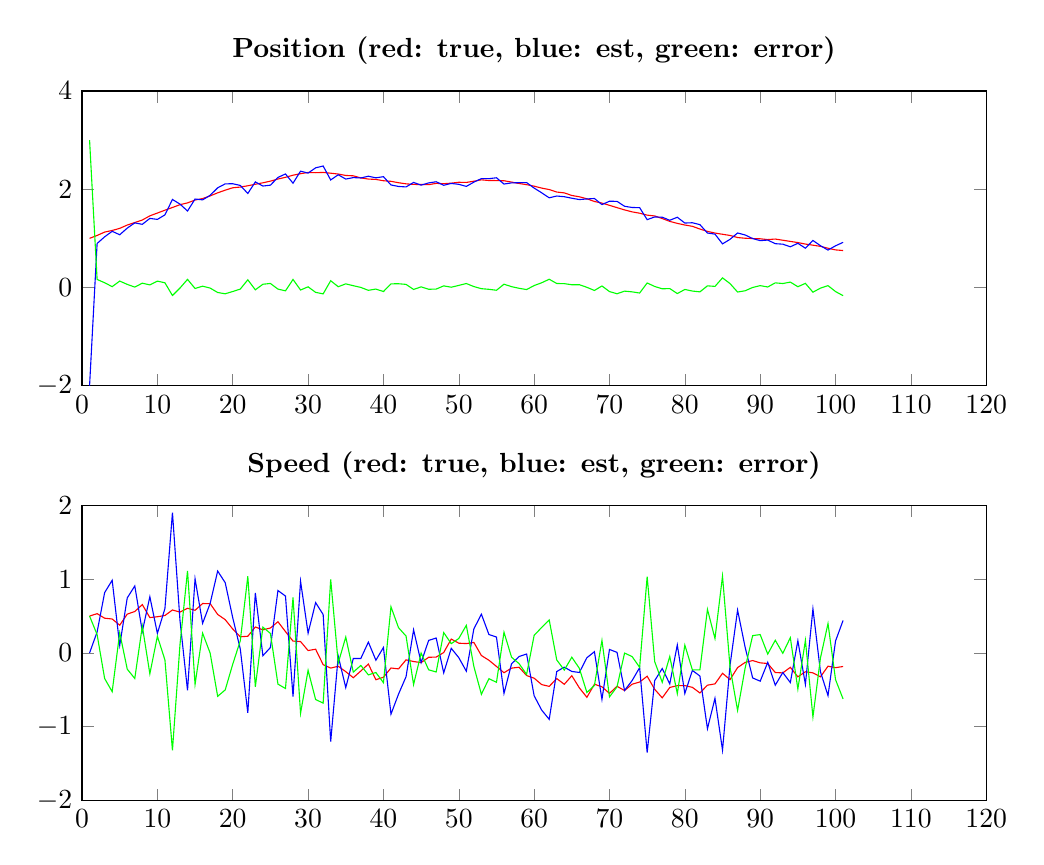
\begin{tikzpicture}

\begin{axis}[%
width=4.521in,
height=1.474in,
at={(0.758in,2.554in)},
scale only axis,
xmin=0,
xmax=120,
ymin=-2,
ymax=4,
axis background/.style={fill=white},
title style={font=\bfseries},
title={Position (red: true, blue: est, green: error)}
]
\addplot [color=red,solid,forget plot]
  table[row sep=crcr]{%
1	1\\
2	1.05870598427715\\
3	1.12749230731841\\
4	1.16039759421018\\
5	1.20321534229327\\
6	1.2709892482814\\
7	1.32249789987429\\
8	1.37304075861392\\
9	1.45819994460386\\
10	1.5148803758713\\
11	1.57323239131671\\
12	1.62803560458185\\
13	1.6854254655997\\
14	1.72154110104229\\
15	1.77944215815875\\
16	1.80957945543787\\
17	1.86367919451911\\
18	1.92637991734311\\
19	1.9806015326155\\
20	2.02945267459007\\
21	2.04400241076363\\
22	2.07004093881062\\
23	2.10085902417589\\
24	2.13040416054477\\
25	2.16421567986312\\
26	2.20724184313826\\
27	2.24205948391006\\
28	2.28549891658137\\
29	2.31592600392495\\
30	2.34123042225401\\
31	2.33614450950653\\
32	2.34176467016137\\
33	2.32585126820625\\
34	2.30905499991248\\
35	2.2801906682252\\
36	2.27268089659063\\
37	2.23019012049038\\
38	2.20643641276986\\
39	2.19920840854875\\
40	2.17245616754435\\
41	2.16075289641942\\
42	2.13202275703047\\
43	2.10958618131336\\
44	2.09735918495331\\
45	2.0960855800506\\
46	2.09228489665458\\
47	2.11904309468798\\
48	2.1126210031341\\
49	2.12327549979068\\
50	2.14146070415507\\
51	2.13765915649916\\
52	2.16291466789521\\
53	2.19115520488701\\
54	2.17707470597472\\
55	2.17605648620464\\
56	2.17233919247631\\
57	2.14536998959949\\
58	2.11662362086678\\
59	2.0927463767804\\
60	2.06228073969808\\
61	2.0230111101413\\
62	1.99272711341757\\
63	1.94249181456348\\
64	1.92551614453321\\
65	1.87264057611182\\
66	1.84590775048055\\
67	1.80511297117557\\
68	1.75040588485229\\
69	1.71746627006423\\
70	1.67208180471905\\
71	1.62495766695363\\
72	1.57862101253843\\
73	1.53911156476134\\
74	1.51172761299487\\
75	1.47211727828008\\
76	1.45594146568592\\
77	1.40313342564925\\
78	1.34552008686516\\
79	1.30447269242715\\
80	1.27138543649242\\
81	1.24489348355257\\
82	1.1894289487338\\
83	1.14161155297534\\
84	1.10807192266353\\
85	1.08296310960671\\
86	1.05889817807817\\
87	1.01642345385874\\
88	1.00208879462559\\
89	0.996075346024873\\
90	0.990812211620114\\
91	0.974675442308043\\
92	0.985672712847739\\
93	0.961580183114868\\
94	0.937790823412868\\
95	0.914182831087925\\
96	0.883412437954006\\
97	0.860804722735173\\
98	0.836856474908927\\
99	0.799106707307957\\
100	0.765041001979168\\
101	0.751664131712262\\
};
\addplot [color=blue,solid,forget plot]
  table[row sep=crcr]{%
1	-2\\
2	0.895528779336162\\
3	1.0308914321479\\
4	1.14367422840011\\
5	1.0728083323019\\
6	1.20818331836287\\
7	1.31444093113683\\
8	1.2852371165813\\
9	1.40601686701958\\
10	1.3855400552569\\
11	1.47757399121603\\
12	1.7914807280425\\
13	1.696769373953\\
14	1.55612891161378\\
15	1.80006254143271\\
16	1.78312434597311\\
17	1.87567058374362\\
18	2.0284476587849\\
19	2.10888465039746\\
20	2.11163166981848\\
21	2.07701968329868\\
22	1.91339379313552\\
23	2.14890209060468\\
24	2.06457855604516\\
25	2.08239735302398\\
26	2.24031344010844\\
27	2.31043591717937\\
28	2.12221569155578\\
29	2.36768200784936\\
30	2.32778553631202\\
31	2.4352899325618\\
32	2.47211147220395\\
33	2.18834435177565\\
34	2.29392895654217\\
35	2.20655841781063\\
36	2.23636485630389\\
37	2.2289382466268\\
38	2.26460612293674\\
39	2.23154904269053\\
40	2.25534652911291\\
41	2.08662133123439\\
42	2.05633000820662\\
43	2.0464610260232\\
44	2.13797567438013\\
45	2.08306489988866\\
46	2.12845163450064\\
47	2.15179491620174\\
48	2.0800618510564\\
49	2.1177783001601\\
50	2.09943331340821\\
51	2.057278662306\\
52	2.14419958985055\\
53	2.21569004487011\\
54	2.21456007504867\\
55	2.23282878900467\\
56	2.10541567383024\\
57	2.12858397032502\\
58	2.13312940003561\\
59	2.1348508364715\\
60	2.02306582041054\\
61	1.92718416059924\\
62	1.82513992803653\\
63	1.8613027457456\\
64	1.84769309772258\\
65	1.81708593136284\\
66	1.78923694165057\\
67	1.80168118309277\\
68	1.81106958470415\\
69	1.68686753786133\\
70	1.75571321795674\\
71	1.75271062297408\\
72	1.65296912984212\\
73	1.62804703538024\\
74	1.62472111679157\\
75	1.38039404946004\\
76	1.43529900559588\\
77	1.4297716015549\\
78	1.36801695589726\\
79	1.42893369542559\\
80	1.31160690036448\\
81	1.31749901141153\\
82	1.27892790375418\\
83	1.10845227883689\\
84	1.08592402686332\\
85	0.887516968021567\\
86	0.980258251529515\\
87	1.10903715119678\\
88	1.06914854737906\\
89	0.995809375997133\\
90	0.953255278133493\\
91	0.964689673820187\\
92	0.891577216622858\\
93	0.881305228473967\\
94	0.828177285726436\\
95	0.898566591016967\\
96	0.799785634023946\\
97	0.956731063831331\\
98	0.85006084248183\\
99	0.761606658914298\\
100	0.848089904915615\\
101	0.918469753665371\\
};
\addplot [color=green,solid,forget plot]
  table[row sep=crcr]{%
1	3\\
2	0.163177204940984\\
3	0.0966008751705076\\
4	0.0167233658100627\\
5	0.130407009991379\\
6	0.0628059299185297\\
7	0.00805696873746675\\
8	0.087803642032624\\
9	0.0521830775842789\\
10	0.129340320614401\\
11	0.0956584001006802\\
12	-0.163445123460652\\
13	-0.0113439083532962\\
14	0.165412189428518\\
15	-0.0206203832739582\\
16	0.0264551094647656\\
17	-0.011991389224514\\
18	-0.102067741441795\\
19	-0.128283117781962\\
20	-0.0821789952284071\\
21	-0.033017272535055\\
22	0.1566471456751\\
23	-0.0480430664287974\\
24	0.0658256044996106\\
25	0.0818183268391395\\
26	-0.033071596970184\\
27	-0.0683764332693091\\
28	0.163283225025582\\
29	-0.0517560039244129\\
30	0.0134448859419831\\
31	-0.099145423055274\\
32	-0.13034680204258\\
33	0.137506916430593\\
34	0.0151260433703104\\
35	0.0736322504145757\\
36	0.0363160402867435\\
37	0.00125187386357828\\
38	-0.058169710166879\\
39	-0.032340634141776\\
40	-0.0828903615685603\\
41	0.074131565185025\\
42	0.075692748823855\\
43	0.0631251552901668\\
44	-0.0406164894268222\\
45	0.0130206801619432\\
46	-0.0361667378460622\\
47	-0.0327518215137603\\
48	0.0325591520777038\\
49	0.0054971996305806\\
50	0.0420273907468593\\
51	0.080380494193157\\
52	0.0187150780446599\\
53	-0.0245348399831067\\
54	-0.0374853690739445\\
55	-0.0567723028000255\\
56	0.0669235186460737\\
57	0.016786019274464\\
58	-0.0165057791688383\\
59	-0.0421044596911022\\
60	0.0392149192875393\\
61	0.0958269495420594\\
62	0.167587185381041\\
63	0.0811890688178716\\
64	0.0778230468106251\\
65	0.0555546447489841\\
66	0.0566708088299832\\
67	0.00343178808280098\\
68	-0.0606636998518602\\
69	0.0305987322029024\\
70	-0.0836314132376901\\
71	-0.127752956020446\\
72	-0.0743481173036897\\
73	-0.0889354706188974\\
74	-0.112993503796706\\
75	0.0917232288200391\\
76	0.0206424600900459\\
77	-0.0266381759056569\\
78	-0.0224968690321015\\
79	-0.124461002998433\\
80	-0.0402214638720597\\
81	-0.0726055278589597\\
82	-0.089498955020378\\
83	0.0331592741384557\\
84	0.0221478958002033\\
85	0.195446141585144\\
86	0.0786399265486555\\
87	-0.0926136973380354\\
88	-0.0670597527534649\\
89	0.000265970027739315\\
90	0.0375569334866215\\
91	0.00998576848785548\\
92	0.094095496224881\\
93	0.0802749546409011\\
94	0.109613537686433\\
95	0.015616240070958\\
96	0.0836268039300604\\
97	-0.0959263410961573\\
98	-0.0132043675729029\\
99	0.0375000483936588\\
100	-0.0830489029364468\\
101	-0.166805621953109\\
};
\end{axis}

\begin{axis}[%
width=4.521in,
height=1.474in,
at={(0.758in,0.481in)},
scale only axis,
xmin=0,
xmax=120,
ymin=-2,
ymax=2,
axis background/.style={fill=white},
title style={font=\bfseries},
title={Speed (red: true, blue: est, green: error)}
]
\addplot [color=red,solid,forget plot]
  table[row sep=crcr]{%
1	0.5\\
2	0.533076051889906\\
3	0.47141237733062\\
4	0.460449141266709\\
5	0.376490402582667\\
6	0.526574448874078\\
7	0.562464563496022\\
8	0.655868040446716\\
9	0.479545093408841\\
10	0.49133663247586\\
11	0.507661123790698\\
12	0.583276864544189\\
13	0.553856255645857\\
14	0.605994322363615\\
15	0.578491116564894\\
16	0.670298607437167\\
17	0.669426798169673\\
18	0.522481930576498\\
19	0.451794377659234\\
20	0.325042821374648\\
21	0.219258873649497\\
22	0.22630865227049\\
23	0.35248436317666\\
24	0.31309460601885\\
25	0.338307086915332\\
26	0.42352284176031\\
27	0.289672659188171\\
28	0.160660061784845\\
29	0.154492841509254\\
30	0.032635001954966\\
31	0.0506030123198061\\
32	-0.159401172252215\\
33	-0.205354851434248\\
34	-0.180836800640745\\
35	-0.253853033885956\\
36	-0.335893386805726\\
37	-0.244818525442917\\
38	-0.150876894619148\\
39	-0.36415096391694\\
40	-0.329151553081663\\
41	-0.204292886558714\\
42	-0.216470760515395\\
43	-0.0936594835460313\\
44	-0.11642004903965\\
45	-0.131366301330092\\
46	-0.0590378924298898\\
47	-0.055867816650487\\
48	0.00577429244967283\\
49	0.188684516115827\\
50	0.13233797543129\\
51	0.126965970589642\\
52	0.142550125643639\\
53	-0.0350147120077366\\
54	-0.0993516281022968\\
55	-0.183013869172835\\
56	-0.268522087048496\\
57	-0.205831013570305\\
58	-0.194316259950491\\
59	-0.306365234218912\\
60	-0.342663797105101\\
61	-0.429383114422108\\
62	-0.45352890017619\\
63	-0.347490467745366\\
64	-0.425442346947601\\
65	-0.309058495097953\\
66	-0.473870997217637\\
67	-0.601911156994774\\
68	-0.424066485727525\\
69	-0.459491985163228\\
70	-0.548824254500149\\
71	-0.45257469256549\\
72	-0.510290447326641\\
73	-0.42445256099652\\
74	-0.394918766539442\\
75	-0.315968731191189\\
76	-0.493459409477354\\
77	-0.609357693889756\\
78	-0.468236757785875\\
79	-0.443927959189694\\
80	-0.442862643084844\\
81	-0.466809870057835\\
82	-0.543004471989484\\
83	-0.437195244947464\\
84	-0.420002677497369\\
85	-0.276298228246866\\
86	-0.361322382870257\\
87	-0.198874646578018\\
88	-0.128532885026517\\
89	-0.103403927070346\\
90	-0.134393838887606\\
91	-0.143206856103352\\
92	-0.265531161870032\\
93	-0.270592309599819\\
94	-0.195293218271599\\
95	-0.324083861389714\\
96	-0.255826390036361\\
97	-0.270157215595324\\
98	-0.323875635773651\\
99	-0.179973508561884\\
100	-0.200097810757886\\
101	-0.183689374180793\\
};
\addplot [color=blue,solid,forget plot]
  table[row sep=crcr]{%
1	0\\
2	0.283875370523153\\
3	0.818750949320283\\
4	0.985880554351189\\
5	0.102209577466225\\
6	0.746453911478767\\
7	0.908827284888686\\
8	0.292105281511844\\
9	0.762382068508568\\
10	0.265674675553923\\
11	0.60189633276486\\
12	1.9049323013088\\
13	0.440183579978608\\
14	-0.508183952844229\\
15	1.00559833050427\\
16	0.402154015401573\\
17	0.670913806772194\\
18	1.11097689384658\\
19	0.953510219700306\\
20	0.477916206726252\\
21	0.0547092054150477\\
22	-0.813735230791485\\
23	0.813700868348288\\
24	-0.0372655278550954\\
25	0.0733867017817741\\
26	0.846719559957361\\
27	0.771996601142808\\
28	-0.59114219530797\\
29	0.973117181383998\\
30	0.268445766060994\\
31	0.682697053847374\\
32	0.521186115502402\\
33	-1.20384993882852\\
34	-0.0433192352565359\\
35	-0.469787499591792\\
36	-0.0754354747564027\\
37	-0.0748349076604964\\
38	0.146781126939383\\
39	-0.0983764401807168\\
40	0.0743662731228091\\
41	-0.830362540634276\\
42	-0.559476048422349\\
43	-0.322826265914054\\
44	0.312969608640857\\
45	-0.129774567405482\\
46	0.169971223438103\\
47	0.20256371741921\\
48	-0.269874020002345\\
49	0.0624308842604022\\
50	-0.0638481212176808\\
51	-0.247554233220136\\
52	0.325991211911295\\
53	0.525728642435312\\
54	0.249922568637106\\
55	0.215391914833144\\
56	-0.549594730615618\\
57	-0.14834750128179\\
58	-0.0488151133938925\\
59	-0.0149038099570837\\
60	-0.581353063297185\\
61	-0.775210123826968\\
62	-0.901156048143601\\
63	-0.252617539366243\\
64	-0.192774858072679\\
65	-0.250961632848594\\
66	-0.265099550558332\\
67	-0.065039271037774\\
68	0.0165802721903624\\
69	-0.629809689891589\\
70	0.047223303599906\\
71	0.00754976744046996\\
72	-0.508578240879237\\
73	-0.375377975310456\\
74	-0.19967320716096\\
75	-1.35193606087728\\
76	-0.375631197373659\\
77	-0.211102730275489\\
78	-0.419843386746887\\
79	0.108634166866699\\
80	-0.549722875496043\\
81	-0.237136564115842\\
82	-0.313441201777728\\
83	-1.02799034489024\\
84	-0.615737067167287\\
85	-1.31848339836814\\
86	-0.165039947775034\\
87	0.581101394753885\\
88	0.0778011668343105\\
89	-0.338809850817777\\
90	-0.383353071406106\\
91	-0.127746704071863\\
92	-0.437628451767473\\
93	-0.265626695327325\\
94	-0.40206015982354\\
95	0.165933352470779\\
96	-0.426603915143193\\
97	0.598528162977577\\
98	-0.2566979346781\\
99	-0.579144904762906\\
100	0.162450458994798\\
101	0.440475030508275\\
};
\addplot [color=green,solid,forget plot]
  table[row sep=crcr]{%
1	0.5\\
2	0.249200681366753\\
3	-0.347338571989664\\
4	-0.525431413084481\\
5	0.274280825116442\\
6	-0.219879462604689\\
7	-0.346362721392664\\
8	0.363762758934872\\
9	-0.282836975099727\\
10	0.225661956921937\\
11	-0.0942352089741624\\
12	-1.32165543676461\\
13	0.113672675667249\\
14	1.11417827520784\\
15	-0.427107213939378\\
16	0.268144592035593\\
17	-0.00148700860252104\\
18	-0.588494963270079\\
19	-0.501715842041071\\
20	-0.152873385351604\\
21	0.164549668234449\\
22	1.04004388306198\\
23	-0.461216505171628\\
24	0.350360133873946\\
25	0.264920385133558\\
26	-0.423196718197051\\
27	-0.482323941954637\\
28	0.751802257092814\\
29	-0.818624339874744\\
30	-0.235810764106028\\
31	-0.632094041527568\\
32	-0.680587287754617\\
33	0.998495087394276\\
34	-0.137517565384209\\
35	0.215934465705836\\
36	-0.260457912049323\\
37	-0.16998361778242\\
38	-0.297658021558531\\
39	-0.265774523736223\\
40	-0.403517826204472\\
41	0.626069654075562\\
42	0.343005287906954\\
43	0.229166782368023\\
44	-0.429389657680508\\
45	-0.00159173392460998\\
46	-0.229009115867993\\
47	-0.258431534069697\\
48	0.275648312452018\\
49	0.126253631855425\\
50	0.196186096648971\\
51	0.374520203809777\\
52	-0.183441086267655\\
53	-0.560743354443048\\
54	-0.349274196739403\\
55	-0.398405784005979\\
56	0.281072643567122\\
57	-0.0574835122885149\\
58	-0.145501146556599\\
59	-0.291461424261828\\
60	0.238689266192084\\
61	0.34582700940486\\
62	0.447627147967412\\
63	-0.094872928379123\\
64	-0.232667488874922\\
65	-0.0580968622493588\\
66	-0.208771446659306\\
67	-0.536871885957001\\
68	-0.440646757917887\\
69	0.170317704728361\\
70	-0.596047558100055\\
71	-0.46012446000596\\
72	-0.00171220644740466\\
73	-0.0490745856860639\\
74	-0.195245559378481\\
75	1.03596732968609\\
76	-0.117828212103696\\
77	-0.398254963614268\\
78	-0.0483933710389885\\
79	-0.552562126056393\\
80	0.106860232411199\\
81	-0.229673305941993\\
82	-0.229563270211755\\
83	0.590795099942773\\
84	0.195734389669918\\
85	1.04218517012128\\
86	-0.196282435095223\\
87	-0.779976041331903\\
88	-0.206334051860828\\
89	0.235405923747431\\
90	0.248959232518501\\
91	-0.0154601520314895\\
92	0.172097289897442\\
93	-0.00496561427249448\\
94	0.206766941551941\\
95	-0.490017213860493\\
96	0.170777525106832\\
97	-0.868685378572901\\
98	-0.0671777010955504\\
99	0.399171396201022\\
100	-0.362548269752684\\
101	-0.624164404689068\\
};
\end{axis}
\end{tikzpicture}%}
	\scalebox{0.5}{% This file was created by matlab2tikz.
%
%The latest updates can be retrieved from
%  http://www.mathworks.com/matlabcentral/fileexchange/22022-matlab2tikz-matlab2tikz
%where you can also make suggestions and rate matlab2tikz.
%
\definecolor{mycolor1}{rgb}{0.00000,0.44700,0.74100}%
%
\begin{tikzpicture}

\begin{axis}[%
width=4.521in,
height=1.474in,
at={(0.758in,2.554in)},
scale only axis,
xmin=0,
xmax=120,
ymin=0,
ymax=1,
axis background/.style={fill=white},
title style={font=\bfseries},
title={sqrt(P(1,1))}
]
\addplot [color=mycolor1,solid,forget plot]
  table[row sep=crcr]{%
1	1\\
2	0.0995133791073302\\
3	0.0894427190999916\\
4	0.090955874798141\\
5	0.0908951808652624\\
6	0.0907222446551644\\
7	0.0906668510238416\\
8	0.0906568017937734\\
9	0.0906557581243606\\
10	0.0906557389997454\\
11	0.0906557478190609\\
12	0.0906557467287357\\
13	0.0906557455733183\\
14	0.0906557452449743\\
15	0.0906557451906057\\
16	0.0906557451856966\\
17	0.0906557451857197\\
18	0.0906557451857654\\
19	0.0906557451857541\\
20	0.0906557451857466\\
21	0.0906557451857446\\
22	0.0906557451857443\\
23	0.0906557451857443\\
24	0.0906557451857443\\
25	0.0906557451857443\\
26	0.0906557451857443\\
27	0.0906557451857443\\
28	0.0906557451857443\\
29	0.0906557451857443\\
30	0.0906557451857443\\
31	0.0906557451857443\\
32	0.0906557451857443\\
33	0.0906557451857443\\
34	0.0906557451857443\\
35	0.0906557451857443\\
36	0.0906557451857443\\
37	0.0906557451857443\\
38	0.0906557451857443\\
39	0.0906557451857443\\
40	0.0906557451857443\\
41	0.0906557451857443\\
42	0.0906557451857443\\
43	0.0906557451857443\\
44	0.0906557451857443\\
45	0.0906557451857443\\
46	0.0906557451857443\\
47	0.0906557451857443\\
48	0.0906557451857443\\
49	0.0906557451857443\\
50	0.0906557451857443\\
51	0.0906557451857443\\
52	0.0906557451857443\\
53	0.0906557451857443\\
54	0.0906557451857443\\
55	0.0906557451857443\\
56	0.0906557451857443\\
57	0.0906557451857443\\
58	0.0906557451857443\\
59	0.0906557451857443\\
60	0.0906557451857443\\
61	0.0906557451857443\\
62	0.0906557451857443\\
63	0.0906557451857443\\
64	0.0906557451857443\\
65	0.0906557451857443\\
66	0.0906557451857443\\
67	0.0906557451857443\\
68	0.0906557451857443\\
69	0.0906557451857443\\
70	0.0906557451857443\\
71	0.0906557451857443\\
72	0.0906557451857443\\
73	0.0906557451857443\\
74	0.0906557451857443\\
75	0.0906557451857443\\
76	0.0906557451857443\\
77	0.0906557451857443\\
78	0.0906557451857443\\
79	0.0906557451857443\\
80	0.0906557451857443\\
81	0.0906557451857443\\
82	0.0906557451857443\\
83	0.0906557451857443\\
84	0.0906557451857443\\
85	0.0906557451857443\\
86	0.0906557451857443\\
87	0.0906557451857443\\
88	0.0906557451857443\\
89	0.0906557451857443\\
90	0.0906557451857443\\
91	0.0906557451857443\\
92	0.0906557451857443\\
93	0.0906557451857443\\
94	0.0906557451857443\\
95	0.0906557451857443\\
96	0.0906557451857443\\
97	0.0906557451857443\\
98	0.0906557451857443\\
99	0.0906557451857443\\
100	0.0906557451857443\\
101	0.0906557451857443\\
};
\end{axis}

\begin{axis}[%
width=4.521in,
height=1.474in,
at={(0.758in,0.481in)},
scale only axis,
xmin=0,
xmax=120,
ymin=1,
ymax=1.6,
axis background/.style={fill=white},
title style={font=\bfseries},
title={sqrt(P(2,2))}
]
\addplot [color=mycolor1,solid,forget plot]
  table[row sep=crcr]{%
1	1\\
2	1.41077682931636\\
3	1.47996326377918\\
4	1.42531486631628\\
5	1.40125423630035\\
6	1.39609549130694\\
7	1.39542646845987\\
8	1.39539023753365\\
9	1.39539385790114\\
10	1.39539404315567\\
11	1.39539365741493\\
12	1.39539351311409\\
13	1.39539348442171\\
14	1.39539348106616\\
15	1.39539348094124\\
16	1.39539348096507\\
17	1.39539348096424\\
18	1.39539348096153\\
19	1.39539348096066\\
20	1.3953934809605\\
21	1.39539348096048\\
22	1.39539348096048\\
23	1.39539348096048\\
24	1.39539348096048\\
25	1.39539348096048\\
26	1.39539348096048\\
27	1.39539348096048\\
28	1.39539348096048\\
29	1.39539348096048\\
30	1.39539348096048\\
31	1.39539348096048\\
32	1.39539348096048\\
33	1.39539348096048\\
34	1.39539348096048\\
35	1.39539348096048\\
36	1.39539348096048\\
37	1.39539348096048\\
38	1.39539348096048\\
39	1.39539348096048\\
40	1.39539348096048\\
41	1.39539348096048\\
42	1.39539348096048\\
43	1.39539348096048\\
44	1.39539348096048\\
45	1.39539348096048\\
46	1.39539348096048\\
47	1.39539348096048\\
48	1.39539348096048\\
49	1.39539348096048\\
50	1.39539348096048\\
51	1.39539348096048\\
52	1.39539348096048\\
53	1.39539348096048\\
54	1.39539348096048\\
55	1.39539348096048\\
56	1.39539348096048\\
57	1.39539348096048\\
58	1.39539348096048\\
59	1.39539348096048\\
60	1.39539348096048\\
61	1.39539348096048\\
62	1.39539348096048\\
63	1.39539348096048\\
64	1.39539348096048\\
65	1.39539348096048\\
66	1.39539348096048\\
67	1.39539348096048\\
68	1.39539348096048\\
69	1.39539348096048\\
70	1.39539348096048\\
71	1.39539348096048\\
72	1.39539348096048\\
73	1.39539348096048\\
74	1.39539348096048\\
75	1.39539348096048\\
76	1.39539348096048\\
77	1.39539348096048\\
78	1.39539348096048\\
79	1.39539348096048\\
80	1.39539348096048\\
81	1.39539348096048\\
82	1.39539348096048\\
83	1.39539348096048\\
84	1.39539348096048\\
85	1.39539348096048\\
86	1.39539348096048\\
87	1.39539348096048\\
88	1.39539348096048\\
89	1.39539348096048\\
90	1.39539348096048\\
91	1.39539348096048\\
92	1.39539348096048\\
93	1.39539348096048\\
94	1.39539348096048\\
95	1.39539348096048\\
96	1.39539348096048\\
97	1.39539348096048\\
98	1.39539348096048\\
99	1.39539348096048\\
100	1.39539348096048\\
101	1.39539348096048\\
};
\end{axis}
\end{tikzpicture}%}
	\scalebox{0.5}{% This file was created by matlab2tikz.
%
%The latest updates can be retrieved from
%  http://www.mathworks.com/matlabcentral/fileexchange/22022-matlab2tikz-matlab2tikz
%where you can also make suggestions and rate matlab2tikz.
%
\definecolor{mycolor1}{rgb}{0.00000,0.44700,0.74100}%
%
\begin{tikzpicture}

\begin{axis}[%
width=4.521in,
height=1.474in,
at={(0.758in,2.554in)},
scale only axis,
xmin=0,
xmax=100,
ymin=0.8,
ymax=1,
axis background/.style={fill=white},
title style={font=\bfseries},
title={K(1)}
]
\addplot [color=mycolor1,solid,forget plot]
  table[row sep=crcr]{%
1	0.990291262135922\\
2	0.8\\
3	0.827297116029511\\
4	0.826193390452876\\
5	0.82305256752715\\
6	0.822047787457949\\
7	0.821865571147552\\
8	0.821846648110258\\
9	0.821846301358995\\
10	0.821846461263315\\
11	0.821846441494467\\
12	0.821846420545421\\
13	0.821846414592167\\
14	0.821846413606404\\
15	0.821846413517395\\
16	0.821846413517813\\
17	0.821846413518643\\
18	0.821846413518437\\
19	0.8218464135183\\
20	0.821846413518266\\
21	0.82184641351826\\
22	0.82184641351826\\
23	0.82184641351826\\
24	0.82184641351826\\
25	0.82184641351826\\
26	0.82184641351826\\
27	0.82184641351826\\
28	0.82184641351826\\
29	0.82184641351826\\
30	0.82184641351826\\
31	0.82184641351826\\
32	0.82184641351826\\
33	0.82184641351826\\
34	0.82184641351826\\
35	0.82184641351826\\
36	0.82184641351826\\
37	0.82184641351826\\
38	0.82184641351826\\
39	0.82184641351826\\
40	0.82184641351826\\
41	0.82184641351826\\
42	0.82184641351826\\
43	0.82184641351826\\
44	0.82184641351826\\
45	0.82184641351826\\
46	0.82184641351826\\
47	0.82184641351826\\
48	0.82184641351826\\
49	0.82184641351826\\
50	0.82184641351826\\
51	0.82184641351826\\
52	0.82184641351826\\
53	0.82184641351826\\
54	0.82184641351826\\
55	0.82184641351826\\
56	0.82184641351826\\
57	0.82184641351826\\
58	0.82184641351826\\
59	0.82184641351826\\
60	0.82184641351826\\
61	0.82184641351826\\
62	0.82184641351826\\
63	0.82184641351826\\
64	0.82184641351826\\
65	0.82184641351826\\
66	0.82184641351826\\
67	0.82184641351826\\
68	0.82184641351826\\
69	0.82184641351826\\
70	0.82184641351826\\
71	0.82184641351826\\
72	0.82184641351826\\
73	0.82184641351826\\
74	0.82184641351826\\
75	0.82184641351826\\
76	0.82184641351826\\
77	0.82184641351826\\
78	0.82184641351826\\
79	0.82184641351826\\
80	0.82184641351826\\
81	0.82184641351826\\
82	0.82184641351826\\
83	0.82184641351826\\
84	0.82184641351826\\
85	0.82184641351826\\
86	0.82184641351826\\
87	0.82184641351826\\
88	0.82184641351826\\
89	0.82184641351826\\
90	0.82184641351826\\
91	0.82184641351826\\
92	0.82184641351826\\
93	0.82184641351826\\
94	0.82184641351826\\
95	0.82184641351826\\
96	0.82184641351826\\
97	0.82184641351826\\
98	0.82184641351826\\
99	0.82184641351826\\
100	0.82184641351826\\
};
\end{axis}

\begin{axis}[%
width=4.521in,
height=1.474in,
at={(0.758in,0.481in)},
scale only axis,
xmin=0,
xmax=100,
ymin=0,
ymax=6,
axis background/.style={fill=white},
title style={font=\bfseries},
title={K(2)}
]
\addplot [color=mycolor1,solid,forget plot]
  table[row sep=crcr]{%
1	0.0970873786407767\\
2	4\\
3	4.47350771294433\\
4	4.30844553243574\\
5	4.23675498396262\\
6	4.22237557146554\\
7	4.2208108310451\\
8	4.22080030193479\\
9	4.22082464139959\\
10	4.22082611016637\\
11	4.22082492233775\\
12	4.22082448960039\\
13	4.22082441089625\\
14	4.22082440354614\\
15	4.22082440372439\\
16	4.22082440386476\\
17	4.22082440386594\\
18	4.22082440385757\\
19	4.22082440385499\\
20	4.22082440385456\\
21	4.22082440385453\\
22	4.22082440385453\\
23	4.22082440385453\\
24	4.22082440385454\\
25	4.22082440385454\\
26	4.22082440385453\\
27	4.22082440385453\\
28	4.22082440385453\\
29	4.22082440385453\\
30	4.22082440385453\\
31	4.22082440385453\\
32	4.22082440385453\\
33	4.22082440385453\\
34	4.22082440385453\\
35	4.22082440385453\\
36	4.22082440385453\\
37	4.22082440385453\\
38	4.22082440385453\\
39	4.22082440385453\\
40	4.22082440385453\\
41	4.22082440385453\\
42	4.22082440385453\\
43	4.22082440385453\\
44	4.22082440385453\\
45	4.22082440385453\\
46	4.22082440385453\\
47	4.22082440385453\\
48	4.22082440385453\\
49	4.22082440385453\\
50	4.22082440385453\\
51	4.22082440385453\\
52	4.22082440385453\\
53	4.22082440385453\\
54	4.22082440385453\\
55	4.22082440385453\\
56	4.22082440385453\\
57	4.22082440385453\\
58	4.22082440385453\\
59	4.22082440385453\\
60	4.22082440385453\\
61	4.22082440385453\\
62	4.22082440385453\\
63	4.22082440385453\\
64	4.22082440385453\\
65	4.22082440385453\\
66	4.22082440385453\\
67	4.22082440385453\\
68	4.22082440385453\\
69	4.22082440385453\\
70	4.22082440385453\\
71	4.22082440385453\\
72	4.22082440385453\\
73	4.22082440385453\\
74	4.22082440385453\\
75	4.22082440385453\\
76	4.22082440385453\\
77	4.22082440385453\\
78	4.22082440385453\\
79	4.22082440385453\\
80	4.22082440385453\\
81	4.22082440385453\\
82	4.22082440385453\\
83	4.22082440385453\\
84	4.22082440385453\\
85	4.22082440385453\\
86	4.22082440385453\\
87	4.22082440385453\\
88	4.22082440385453\\
89	4.22082440385453\\
90	4.22082440385453\\
91	4.22082440385453\\
92	4.22082440385453\\
93	4.22082440385453\\
94	4.22082440385453\\
95	4.22082440385453\\
96	4.22082440385453\\
97	4.22082440385453\\
98	4.22082440385453\\
99	4.22082440385453\\
100	4.22082440385453\\
};
\end{axis}
\end{tikzpicture}%}

	\caption{$Q$ default, $R \times 100$.}
	\label{fig:q3:Rx100}
\end{figure}

\begin{figure}[H]
	\scalebox{0.5}{% This file was created by matlab2tikz.
%
%The latest updates can be retrieved from
%  http://www.mathworks.com/matlabcentral/fileexchange/22022-matlab2tikz-matlab2tikz
%where you can also make suggestions and rate matlab2tikz.
%
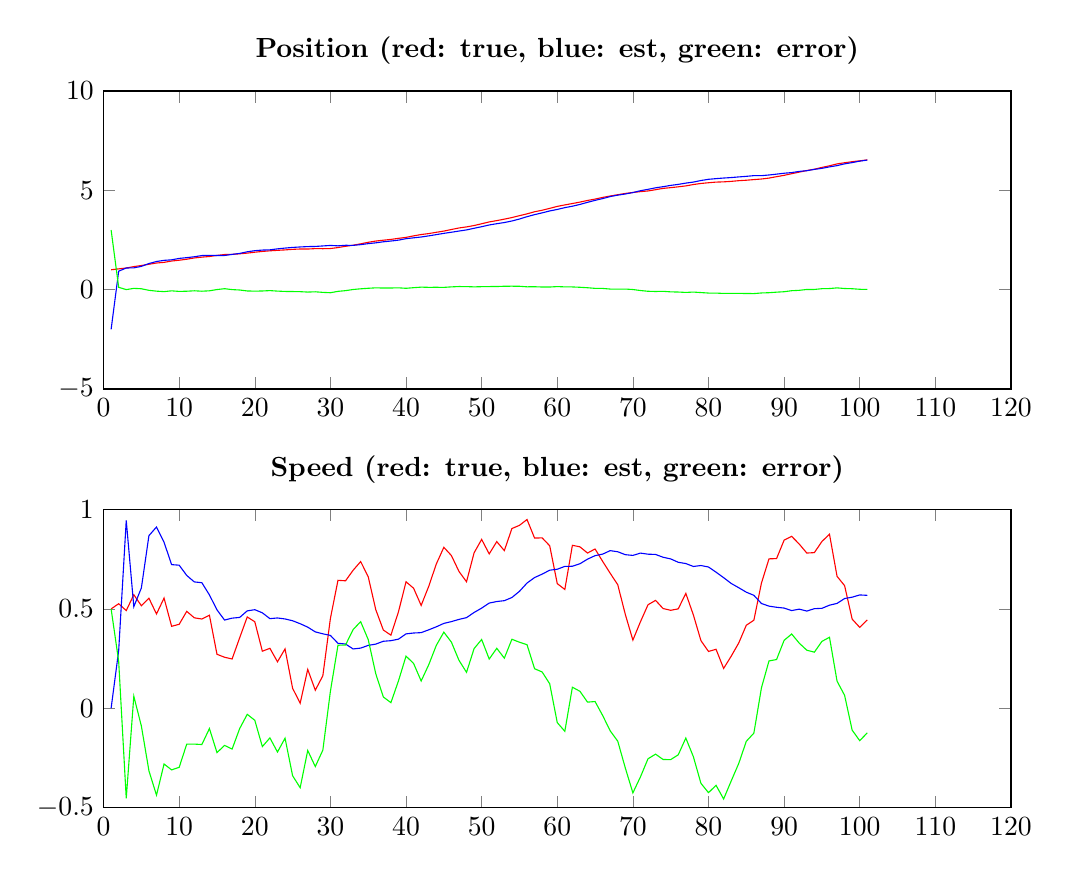
\begin{tikzpicture}

\begin{axis}[%
width=4.537in,
height=1.49in,
at={(0.761in,2.579in)},
scale only axis,
xmin=0,
xmax=120,
ymin=-5,
ymax=10,
axis background/.style={fill=white},
title style={font=\bfseries},
title={Position (red: true, blue: est, green: error)}
]
\addplot [color=red,solid,forget plot]
  table[row sep=crcr]{%
1	1\\
2	1.04412288522635\\
3	1.0888340829712\\
4	1.15852231608985\\
5	1.21360714434405\\
6	1.27700141625339\\
7	1.33840183784133\\
8	1.37233499602073\\
9	1.43877422109731\\
10	1.4801908698245\\
11	1.52943884434963\\
12	1.59496013850499\\
13	1.63470343196013\\
14	1.66732494831453\\
15	1.72201303413315\\
16	1.76540638768067\\
17	1.77420123030285\\
18	1.80236368719307\\
19	1.83708576904105\\
20	1.88328718923431\\
21	1.92174418011591\\
22	1.95289526626406\\
23	1.97708223195751\\
24	1.99913572212049\\
25	2.02706625392485\\
26	2.04415329792344\\
27	2.04225823466477\\
28	2.06383233877895\\
29	2.05932353708755\\
30	2.06738336330698\\
31	2.11666037663612\\
32	2.18013070439576\\
33	2.23388171916447\\
34	2.30438371275335\\
35	2.38184372839689\\
36	2.44427729985365\\
37	2.4876662277591\\
38	2.52741340526044\\
39	2.58097448882325\\
40	2.63036538809022\\
41	2.70504236738086\\
42	2.77295053904033\\
43	2.82115312716976\\
44	2.88491629708122\\
45	2.94609192089574\\
46	3.02619020899178\\
47	3.10280197083505\\
48	3.15678190923007\\
49	3.22621870022284\\
50	3.3148968779275\\
51	3.40736881295415\\
52	3.47305696705603\\
53	3.54721341223225\\
54	3.62669944554185\\
55	3.72208933898024\\
56	3.81255943520208\\
57	3.91900473527662\\
58	3.99540699914109\\
59	4.089850630444\\
60	4.18931898029778\\
61	4.26398452224389\\
62	4.33300051634624\\
63	4.40591786783076\\
64	4.48821868045136\\
65	4.5572306793834\\
66	4.64113005434718\\
67	4.71188221103032\\
68	4.77783481306401\\
69	4.84119606134141\\
70	4.89031588144166\\
71	4.93236306121001\\
72	4.96578208772417\\
73	5.03038818823264\\
74	5.09606570898785\\
75	5.13294141205271\\
76	5.17480121217042\\
77	5.22049578857179\\
78	5.28978360487509\\
79	5.34328969881433\\
80	5.37964278245343\\
81	5.41198449066544\\
82	5.42399346290513\\
83	5.44854595945411\\
84	5.48299992237048\\
85	5.50633400473229\\
86	5.53796592445721\\
87	5.56763926931302\\
88	5.61424059989159\\
89	5.68514535788747\\
90	5.75177497958546\\
91	5.83591492127518\\
92	5.9138523457413\\
93	5.99407157166355\\
94	6.06083730027119\\
95	6.15147355154859\\
96	6.23172071531649\\
97	6.32904269059049\\
98	6.38576517995802\\
99	6.43966768679842\\
100	6.48326274548367\\
101	6.5296083120513\\
};
\addplot [color=blue,solid,forget plot]
  table[row sep=crcr]{%
1	-2\\
2	0.927949958828349\\
3	1.08804807579383\\
4	1.09527931619975\\
5	1.17003770834925\\
6	1.31246735971118\\
7	1.41553175957071\\
8	1.47303832463257\\
9	1.49996808778927\\
10	1.57059567374892\\
11	1.60991911377004\\
12	1.65404951171808\\
13	1.7145743152387\\
14	1.72718965256216\\
15	1.71770975779581\\
16	1.71889883924723\\
17	1.77286959400868\\
18	1.82202485626938\\
19	1.90425859851811\\
20	1.96001767344427\\
21	1.99076801555531\\
22	2.00240597930883\\
23	2.05194553237539\\
24	2.09078246990213\\
25	2.12365346771952\\
26	2.14738637308211\\
27	2.16611043277461\\
28	2.17348289958575\\
29	2.19802059463009\\
30	2.22416394904586\\
31	2.2039601780675\\
32	2.23139236828957\\
33	2.22802978958589\\
34	2.26381686911777\\
35	2.3138815133758\\
36	2.35482927364444\\
37	2.40773621243564\\
38	2.44567288213247\\
39	2.49079540461051\\
40	2.56376673902122\\
41	2.6072989596953\\
42	2.64791864650539\\
43	2.7061045854806\\
44	2.76721838237192\\
45	2.83283498205663\\
46	2.88829812444228\\
47	2.94776086226772\\
48	3.00505582268007\\
49	3.08761462961457\\
50	3.16675609109664\\
51	3.25333939659379\\
52	3.31732151733804\\
53	3.37710149802946\\
54	3.45379913200203\\
55	3.55368535248067\\
56	3.67164524933717\\
57	3.77386157270255\\
58	3.86407206410078\\
59	3.95962593050938\\
60	4.03604899320384\\
61	4.12640730443933\\
62	4.19846735702186\\
63	4.28791429638126\\
64	4.39364678821967\\
65	4.49349713808124\\
66	4.58125359138192\\
67	4.68373760173185\\
68	4.75500945756645\\
69	4.8129672282492\\
70	4.88497195029659\\
71	4.9784110048274\\
72	5.04879352538325\\
73	5.12442175863395\\
74	5.18173715990716\\
75	5.24592106748904\\
76	5.29701677434529\\
77	5.36143760709925\\
78	5.41335371749111\\
79	5.49148311121573\\
80	5.55268041190181\\
81	5.58675895463082\\
82	5.61611462093475\\
83	5.64059738281067\\
84	5.67260353508838\\
85	5.70152415997508\\
86	5.73750347879701\\
87	5.7359361315026\\
88	5.76988694929476\\
89	5.81294808275763\\
90	5.85816690579525\\
91	5.89065560414412\\
92	5.9499733659469\\
93	5.9861269691588\\
94	6.05219508487911\\
95	6.10471942175596\\
96	6.17753997180501\\
97	6.24196787409306\\
98	6.32970472535894\\
99	6.39450149866657\\
100	6.46636885783709\\
101	6.52054630834814\\
};
\addplot [color=green,solid,forget plot]
  table[row sep=crcr]{%
1	3\\
2	0.116172926397998\\
3	0.000786007177377535\\
4	0.0632429998901094\\
5	0.0435694359947962\\
6	-0.0354659434577886\\
7	-0.0771299217293799\\
8	-0.10070332861184\\
9	-0.0611938666919591\\
10	-0.0904048039244143\\
11	-0.0804802694204056\\
12	-0.0590893732130899\\
13	-0.0798708832785695\\
14	-0.0598647042476299\\
15	0.00430327633734096\\
16	0.0465075484334392\\
17	0.0013316362941691\\
18	-0.0196611690763053\\
19	-0.0671728294770557\\
20	-0.0767304842099605\\
21	-0.0690238354394062\\
22	-0.0495107130447707\\
23	-0.0748633004178734\\
24	-0.0916467477816463\\
25	-0.0965872137946739\\
26	-0.103233075158664\\
27	-0.123852198109843\\
28	-0.109650560806802\\
29	-0.138697057542542\\
30	-0.156780585738876\\
31	-0.0872998014313802\\
32	-0.0512616638938104\\
33	0.00585192957857883\\
34	0.0405668436355806\\
35	0.0679622150210948\\
36	0.0894480262092023\\
37	0.079930015323463\\
38	0.0817405231279746\\
39	0.0901790842127426\\
40	0.0665986490690011\\
41	0.0977434076855581\\
42	0.125031892534939\\
43	0.115048541689165\\
44	0.1176979147093\\
45	0.113256938839116\\
46	0.137892084549498\\
47	0.155041108567326\\
48	0.151726086549998\\
49	0.138604070608268\\
50	0.148140786830862\\
51	0.154029416360356\\
52	0.155735449717991\\
53	0.17011191420279\\
54	0.172900313539822\\
55	0.168403986499566\\
56	0.140914185864913\\
57	0.145143162574071\\
58	0.131334935040308\\
59	0.130224699934613\\
60	0.153269987093939\\
61	0.13757721780456\\
62	0.134533159324379\\
63	0.118003571449494\\
64	0.094571892231694\\
65	0.0637335413021614\\
66	0.0598764629652546\\
67	0.0281446092984661\\
68	0.0228253554975666\\
69	0.0282288330922071\\
70	0.00534393114507736\\
71	-0.0460479436173857\\
72	-0.0830114376590858\\
73	-0.0940335704013071\\
74	-0.0856714509193157\\
75	-0.112979655436321\\
76	-0.122215562174875\\
77	-0.140941818527455\\
78	-0.123570112616026\\
79	-0.148193412401399\\
80	-0.17303762944838\\
81	-0.174774463965378\\
82	-0.192121158029622\\
83	-0.19205142335656\\
84	-0.189603612717899\\
85	-0.195190155242787\\
86	-0.199537554339803\\
87	-0.168296862189576\\
88	-0.155646349403173\\
89	-0.127802724870163\\
90	-0.106391926209793\\
91	-0.0547406828689452\\
92	-0.0361210202055959\\
93	0.00794460250475559\\
94	0.00864221539208287\\
95	0.0467541297926326\\
96	0.0541807435114841\\
97	0.0870748164974255\\
98	0.0560604545990717\\
99	0.0451661881318568\\
100	0.0168938876465816\\
101	0.00906200370316057\\
};
\end{axis}

\begin{axis}[%
width=4.537in,
height=1.49in,
at={(0.761in,0.486in)},
scale only axis,
xmin=0,
xmax=120,
ymin=-0.5,
ymax=1,
axis background/.style={fill=white},
title style={font=\bfseries},
title={Speed (red: true, blue: est, green: error)}
]
\addplot [color=red,solid,forget plot]
  table[row sep=crcr]{%
1	0.5\\
2	0.525903630775329\\
3	0.491469656768461\\
4	0.571363831471471\\
5	0.515919520981453\\
6	0.55365902743463\\
7	0.474370415243613\\
8	0.554349362892127\\
9	0.412375180552302\\
10	0.422410324489415\\
11	0.487611901498027\\
12	0.45510215743316\\
13	0.448949346455203\\
14	0.468042406064783\\
15	0.271504182679811\\
16	0.256562176484252\\
17	0.247870007610872\\
18	0.354569183610325\\
19	0.459344866907368\\
20	0.435292438189787\\
21	0.286984467825726\\
22	0.301563771061339\\
23	0.233614955815418\\
24	0.298555373602478\\
25	0.10047548008729\\
26	0.0252157855905291\\
27	0.19534926563221\\
28	0.0905682428456801\\
29	0.163426800684854\\
30	0.45219122946722\\
31	0.643809618636163\\
32	0.641341614005823\\
33	0.694278297430975\\
34	0.738169238784344\\
35	0.661799476623298\\
36	0.495883582255137\\
37	0.393424463674641\\
38	0.367951440655188\\
39	0.485251728356534\\
40	0.636507738484963\\
41	0.603922992928808\\
42	0.517549561162581\\
43	0.613137518351353\\
44	0.72561248606806\\
45	0.809821849916904\\
46	0.768518287028135\\
47	0.688466921307476\\
48	0.636602732239928\\
49	0.782099428462115\\
50	0.849720482847307\\
51	0.776736585268689\\
52	0.838613932882339\\
53	0.793262853271339\\
54	0.904328771045202\\
55	0.920532520355256\\
56	0.949829623969219\\
57	0.856445312519432\\
58	0.857436008521726\\
59	0.817709829552315\\
60	0.627161330068573\\
61	0.597766484389218\\
62	0.820072598929427\\
63	0.812322581972822\\
64	0.781076128589104\\
65	0.801473792005074\\
66	0.739261171096904\\
67	0.679292785786394\\
68	0.621492589725001\\
69	0.471908451478847\\
70	0.342931493141965\\
71	0.435146491488003\\
72	0.520817129332645\\
73	0.542832987742031\\
74	0.501661892152635\\
75	0.492911873954462\\
76	0.500114942384882\\
77	0.578047760423073\\
78	0.469551766623145\\
79	0.340205661604048\\
80	0.285703426638816\\
81	0.296628960022699\\
82	0.200272187674318\\
83	0.261722009861752\\
84	0.328463710728933\\
85	0.417667710389686\\
86	0.442896412018434\\
87	0.629536971679485\\
88	0.751938884381213\\
89	0.753098493256632\\
90	0.845914451242681\\
91	0.86503556532657\\
92	0.826164291359794\\
93	0.78100201468417\\
94	0.783214103950597\\
95	0.839232046087681\\
96	0.87579538255939\\
97	0.663902984160788\\
98	0.616778081769482\\
99	0.448398340748466\\
100	0.406842855147431\\
101	0.444434554310389\\
};
\addplot [color=blue,solid,forget plot]
  table[row sep=crcr]{%
1	0\\
2	0.289895748502066\\
3	0.945438459078416\\
4	0.511018351081271\\
5	0.605278418871576\\
6	0.868739977296748\\
7	0.912026509809283\\
8	0.835180561566043\\
9	0.722777911811939\\
10	0.71987491964251\\
11	0.668288724445081\\
12	0.635741126066858\\
13	0.631732912902728\\
14	0.570302243538837\\
15	0.495047367831433\\
16	0.443799730234802\\
17	0.45339420461075\\
18	0.457014854338038\\
19	0.490066366983424\\
20	0.495920336123573\\
21	0.480194167474114\\
22	0.450829522109043\\
23	0.454322625977966\\
24	0.44928274770395\\
25	0.440266826437677\\
26	0.425366882478074\\
27	0.408146152988141\\
28	0.384257267320185\\
29	0.374432874004772\\
30	0.366499093742719\\
31	0.32680280432554\\
32	0.323152716467574\\
33	0.298400322786728\\
34	0.302520656998262\\
35	0.316241487184237\\
36	0.322700081038428\\
37	0.337006821924275\\
38	0.339946852651079\\
39	0.347681002097878\\
40	0.374273734209736\\
41	0.378529894091405\\
42	0.380461754111083\\
43	0.394545185280578\\
44	0.409711934728841\\
45	0.426991134010433\\
46	0.435950018210099\\
47	0.447098024436533\\
48	0.455947049596423\\
49	0.481955392140905\\
50	0.503741373293387\\
51	0.529243940574044\\
52	0.537034683945432\\
53	0.54131698177464\\
54	0.557222677098599\\
55	0.58835538055501\\
56	0.630036818364597\\
57	0.657681525650823\\
58	0.674913087222432\\
59	0.694696214588809\\
60	0.699597907972554\\
61	0.713976587975917\\
62	0.714443470896893\\
63	0.727131588476314\\
64	0.750401843500423\\
65	0.767885587373867\\
66	0.775614205789312\\
67	0.793175152548958\\
68	0.787506300229408\\
69	0.772856586557592\\
70	0.769136012452959\\
71	0.780778318850576\\
72	0.775357051008724\\
73	0.774013283889635\\
74	0.759863464331925\\
75	0.751549165579754\\
76	0.734600655322739\\
77	0.728233003975938\\
78	0.713505067142208\\
79	0.718280403780267\\
80	0.710791658411957\\
81	0.684726817621592\\
82	0.657171047622724\\
83	0.628123668839749\\
84	0.606422287721083\\
85	0.584075999025667\\
86	0.568276348101382\\
87	0.527139764040056\\
88	0.51392194602053\\
89	0.508053066830121\\
90	0.50411761769501\\
91	0.49149152930299\\
92	0.498654923094171\\
93	0.48899541155327\\
94	0.501090041930233\\
95	0.502791556660199\\
96	0.518671166994255\\
97	0.527519798309289\\
98	0.552165418434077\\
99	0.55891435872049\\
100	0.570168843574414\\
101	0.5681685605767\\
};
\addplot [color=green,solid,forget plot]
  table[row sep=crcr]{%
1	0.5\\
2	0.236007882273263\\
3	-0.453968802309955\\
4	0.0603454803901994\\
5	-0.0893588978901231\\
6	-0.315080949862118\\
7	-0.437656094565669\\
8	-0.280831198673916\\
9	-0.310402731259637\\
10	-0.297464595153095\\
11	-0.180676822947055\\
12	-0.180638968633698\\
13	-0.182783566447526\\
14	-0.102259837474054\\
15	-0.223543185151622\\
16	-0.18723755375055\\
17	-0.205524196999878\\
18	-0.102445670727712\\
19	-0.030721500076056\\
20	-0.0606278979337859\\
21	-0.193209699648388\\
22	-0.149265751047704\\
23	-0.220707670162549\\
24	-0.150727374101472\\
25	-0.339791346350387\\
26	-0.400151096887545\\
27	-0.212796887355931\\
28	-0.293689024474505\\
29	-0.211006073319917\\
30	0.0856921357245015\\
31	0.317006814310623\\
32	0.318188897538249\\
33	0.395877974644247\\
34	0.435648581786082\\
35	0.345557989439061\\
36	0.173183501216709\\
37	0.0564176417503659\\
38	0.0280045880041085\\
39	0.137570726258656\\
40	0.262234004275227\\
41	0.225393098837402\\
42	0.137087807051498\\
43	0.218592333070776\\
44	0.315900551339219\\
45	0.382830715906471\\
46	0.332568268818036\\
47	0.241368896870943\\
48	0.180655682643505\\
49	0.30014403632121\\
50	0.345979109553921\\
51	0.247492644694646\\
52	0.301579248936908\\
53	0.251945871496699\\
54	0.347106093946603\\
55	0.332177139800246\\
56	0.319792805604621\\
57	0.198763786868609\\
58	0.182522921299294\\
59	0.123013614963505\\
60	-0.0724365779039812\\
61	-0.116210103586699\\
62	0.105629128032533\\
63	0.0851909934965076\\
64	0.0306742850886814\\
65	0.0335882046312072\\
66	-0.0363530346924076\\
67	-0.113882366762564\\
68	-0.166013710504407\\
69	-0.300948135078745\\
70	-0.426204519310994\\
71	-0.345631827362573\\
72	-0.254539921676079\\
73	-0.231180296147604\\
74	-0.25820157217929\\
75	-0.258637291625293\\
76	-0.234485712937857\\
77	-0.150185243552864\\
78	-0.243953300519063\\
79	-0.378074742176219\\
80	-0.425088231773141\\
81	-0.388097857598894\\
82	-0.456898859948406\\
83	-0.366401658977997\\
84	-0.277958576992151\\
85	-0.166408288635981\\
86	-0.125379936082948\\
87	0.102397207639429\\
88	0.238016938360683\\
89	0.245045426426511\\
90	0.341796833547671\\
91	0.37354403602358\\
92	0.327509368265623\\
93	0.2920066031309\\
94	0.282124062020364\\
95	0.336440489427483\\
96	0.357124215565135\\
97	0.136383185851499\\
98	0.0646126633354052\\
99	-0.110516017972024\\
100	-0.163325988426983\\
101	-0.123734006266311\\
};
\end{axis}
\end{tikzpicture}%}
	\scalebox{0.5}{% This file was created by matlab2tikz.
%
%The latest updates can be retrieved from
%  http://www.mathworks.com/matlabcentral/fileexchange/22022-matlab2tikz-matlab2tikz
%where you can also make suggestions and rate matlab2tikz.
%
\definecolor{mycolor1}{rgb}{0.00000,0.44700,0.74100}%
%
\begin{tikzpicture}

\begin{axis}[%
width=4.521in,
height=1.474in,
at={(0.758in,2.554in)},
scale only axis,
xmin=0,
xmax=120,
ymin=0,
ymax=1,
axis background/.style={fill=white},
title style={font=\bfseries},
title={sqrt(P(1,1))}
]
\addplot [color=mycolor1,solid,forget plot]
  table[row sep=crcr]{%
1	1\\
2	0.0995085970176974\\
3	0.0816510188183531\\
4	0.0815847608379695\\
5	0.0789722863938857\\
6	0.0750025537476456\\
7	0.0709725549249626\\
8	0.0672820430531738\\
9	0.0640021410422097\\
10	0.0611068427614101\\
11	0.0585475118062397\\
12	0.0562756278340811\\
13	0.0542489288124615\\
14	0.0524322592948223\\
15	0.0507968429076637\\
16	0.0493192131840044\\
17	0.0479801959473739\\
18	0.0467640472929122\\
19	0.0456577542180314\\
20	0.0446504761131104\\
21	0.0437331003244485\\
22	0.0428978877101607\\
23	0.0421381886821168\\
24	0.0414482146537304\\
25	0.0408228535092043\\
26	0.040257520599914\\
27	0.039748038947049\\
28	0.0392905439122532\\
29	0.0388814087101578\\
30	0.038517187882935\\
31	0.0381945763264645\\
32	0.0379103817270337\\
33	0.037661508403088\\
34	0.0374449506055299\\
35	0.037257793360012\\
36	0.0370972189727562\\
37	0.0369605173936578\\
38	0.036845098751334\\
39	0.0367485065481103\\
40	0.0366684302232594\\
41	0.0366027160477789\\
42	0.0365493755871912\\
43	0.0365065912424705\\
44	0.0364727186365919\\
45	0.0364462858416141\\
46	0.0364259896289899\\
47	0.0364106890687606\\
48	0.0363993969004541\\
49	0.036391269152505\\
50	0.0363855935030818\\
51	0.0363817768602526\\
52	0.0363793326010193\\
53	0.0363778678544101\\
54	0.0363770711503597\\
55	0.0363767006893276\\
56	0.0363765734220706\\
57	0.0363765550680622\\
58	0.0363765511469168\\
59	0.0363764990510717\\
60	0.0363763611503146\\
61	0.036376118889356\\
62	0.0363757678179471\\
63	0.0363753134781894\\
64	0.0363747680646948\\
65	0.0363741477691228\\
66	0.0363734707203633\\
67	0.0363727554343394\\
68	0.0363720196922765\\
69	0.0363712797726308\\
70	0.0363705499691117\\
71	0.0363698423349111\\
72	0.0363691666010024\\
73	0.0363685302239047\\
74	0.0363679385254448\\
75	0.036367394893632\\
76	0.0363669010197208\\
77	0.036366457151824\\
78	0.036366062350047\\
79	0.0363657147320597\\
80	0.0363654117013384\\
81	0.0363651501530406\\
82	0.0363649266546806\\
83	0.0363647376005066\\
84	0.0363645793398005\\
85	0.0363644482802941\\
86	0.036364340968565\\
87	0.036364254149708\\
88	0.0363641848088064\\
89	0.0363641301968062\\
90	0.0363640878433528\\
91	0.0363640555590236\\
92	0.0363640314292009\\
93	0.0363640138016052\\
94	0.0363640012692644\\
95	0.0363639926504431\\
96	0.0363639869668115\\
97	0.0363639834209016\\
98	0.0363639813736812\\
99	0.0363639803228869\\
100	0.0363639798825849\\
101	0.0363639797642829\\
};
\end{axis}

\begin{axis}[%
width=4.521in,
height=1.474in,
at={(0.758in,0.481in)},
scale only axis,
xmin=0,
xmax=120,
ymin=0,
ymax=1,
axis background/.style={fill=white},
title style={font=\bfseries},
title={sqrt(P(2,2))}
]
\addplot [color=mycolor1,solid,forget plot]
  table[row sep=crcr]{%
1	1\\
2	0.995136215823267\\
3	0.810566659747937\\
4	0.573707087343345\\
5	0.406390335224514\\
6	0.300665389999027\\
7	0.232283470218788\\
8	0.185962634761561\\
9	0.153193763708075\\
10	0.129158803005861\\
11	0.11100838458245\\
12	0.0969789557832891\\
13	0.085932587536573\\
14	0.0771074525566843\\
15	0.0699766385988112\\
16	0.0641649877429277\\
17	0.0593983172702328\\
18	0.055471420007321\\
19	0.0522273434853236\\
20	0.0495436569056535\\
21	0.0473231650168883\\
22	0.0454875155463811\\
23	0.0439727230432211\\
24	0.042725979570219\\
25	0.0417033392173152\\
26	0.040868002234702\\
27	0.0401890155668045\\
28	0.039640266975165\\
29	0.0391996901985004\\
30	0.0388486253408755\\
31	0.0385712963157955\\
32	0.0383543787268425\\
33	0.0381866391192658\\
34	0.0380586315148147\\
35	0.037962440493052\\
36	0.0378914624200233\\
37	0.037840218132634\\
38	0.0378041916948321\\
39	0.0377796908831709\\
40	0.0377637259093161\\
41	0.0377539035868397\\
42	0.0377483347228963\\
43	0.0377455529776221\\
44	0.0377444437979532\\
45	0.037744182310266\\
46	0.0377441792605498\\
47	0.0377440342349266\\
48	0.0377434954903907\\
49	0.0377424257880595\\
50	0.0377407736601374\\
51	0.0377385495665413\\
52	0.0377358064151275\\
53	0.0377326239360676\\
54	0.0377290964197037\\
55	0.0377253233500996\\
56	0.0377214024941789\\
57	0.0377174250385393\\
58	0.0377134724018977\\
59	0.0377096143894398\\
60	0.0377059083948199\\
61	0.0377023993949033\\
62	0.0376991205204566\\
63	0.0376960940219633\\
64	0.0376933324829076\\
65	0.037690840162779\\
66	0.0376886143784852\\
67	0.0376866468557428\\
68	0.0376849250014428\\
69	0.0376834330641405\\
70	0.0376821531629499\\
71	0.0376810661755456\\
72	0.0376801524840056\\
73	0.0376793925831976\\
74	0.0376787675606397\\
75	0.037678259459548\\
76	0.0376778515383981\\
77	0.0376775284410148\\
78	0.0376772762911817\\
79	0.0376770827252144\\
80	0.0376769368750231\\
81	0.0376768293130312\\
82	0.0376767519690225\\
83	0.0376766980276386\\
84	0.0376766618139092\\
85	0.0376766386729159\\
86	0.0376766248484939\\
87	0.037676617364794\\
88	0.0376766139135667\\
89	0.0376766127491956\\
90	0.0376766125928006\\
91	0.0376766125461466\\
92	0.0376766120156135\\
93	0.0376766106461179\\
94	0.0376766082645891\\
95	0.0376766048324024\\
96	0.0376766004060328\\
97	0.0376765951051159\\
98	0.0376765890870625\\
99	0.0376765825273767\\
100	0.0376765756048537\\
101	0.0376765684908793\\
};
\end{axis}
\end{tikzpicture}%}
	\scalebox{0.5}{% This file was created by matlab2tikz.
%
%The latest updates can be retrieved from
%  http://www.mathworks.com/matlabcentral/fileexchange/22022-matlab2tikz-matlab2tikz
%where you can also make suggestions and rate matlab2tikz.
%
\definecolor{mycolor1}{rgb}{0.00000,0.44700,0.74100}%
%
\begin{tikzpicture}

\begin{axis}[%
width=4.521in,
height=1.474in,
at={(0.758in,2.554in)},
scale only axis,
xmin=0,
xmax=100,
ymin=0,
ymax=1,
axis background/.style={fill=white},
title style={font=\bfseries},
title={K(1)}
]
\addplot [color=mycolor1,solid,forget plot]
  table[row sep=crcr]{%
1	0.990196088043051\\
2	0.666688887407506\\
3	0.665607320098868\\
4	0.623662201827791\\
5	0.562538306866847\\
6	0.503710355257684\\
7	0.452687331740913\\
8	0.40962740579869\\
9	0.37340462322677\\
10	0.342781113870178\\
11	0.316694628812\\
12	0.294294627729952\\
13	0.274914181475948\\
14	0.258031924938586\\
15	0.243238478908927\\
16	0.230209920314839\\
17	0.218687611921372\\
18	0.208463052023416\\
19	0.199366501712744\\
20	0.191258406398827\\
21	0.184022876999356\\
22	0.177562694540968\\
23	0.171795449798171\\
24	0.166650536863396\\
25	0.16206679648525\\
26	0.157990660013612\\
27	0.154374684092069\\
28	0.151176394328633\\
29	0.148357376240931\\
30	0.145882566075812\\
31	0.143719704268941\\
32	0.141838921519587\\
33	0.140212432585058\\
34	0.138814316605736\\
35	0.137620365551262\\
36	0.136607984600688\\
37	0.135756130199555\\
38	0.135045273351651\\
39	0.134457377503804\\
40	0.133975882207433\\
41	0.133585685581357\\
42	0.133273120414482\\
43	0.1330259204744\\
44	0.132833175164864\\
45	0.132685272045128\\
46	0.132573827846196\\
47	0.132491609471678\\
48	0.132432447053006\\
49	0.132391141457151\\
50	0.132363368750921\\
51	0.132345584049559\\
52	0.132334926963292\\
53	0.132329130547833\\
54	0.132326435304093\\
55	0.13232550939313\\
56	0.132325375861976\\
57	0.132325347334425\\
58	0.132324968321262\\
59	0.132323965053812\\
60	0.132322202545256\\
61	0.132319648434519\\
62	0.132316343063655\\
63	0.132312375176034\\
64	0.132307862592998\\
65	0.132302937224513\\
66	0.132297733788626\\
67	0.132292381649535\\
68	0.132286999229899\\
69	0.132281690505565\\
70	0.132276543146629\\
71	0.132271627925147\\
72	0.132266999064707\\
73	0.132262695259053\\
74	0.132258741134937\\
75	0.132255148977817\\
76	0.132251920577545\\
77	0.13224904908475\\
78	0.132246520797354\\
79	0.132244316820784\\
80	0.132242414565319\\
81	0.13224078906003\\
82	0.13223941407537\\
83	0.132238263056065\\
84	0.132237309873018\\
85	0.132236529407805\\
86	0.132235897986455\\
87	0.132235393680903\\
88	0.132234996497027\\
89	0.132234688467908\\
90	0.132234453669976\\
91	0.132234278178391\\
92	0.132234149976333\\
93	0.132234058831106\\
94	0.132233996148148\\
95	0.132233954812244\\
96	0.132233929023561\\
97	0.132233914134543\\
98	0.132233906492331\\
99	0.132233903290104\\
100	0.132233902429718\\
};
\end{axis}

\begin{axis}[%
width=4.521in,
height=1.474in,
at={(0.758in,0.481in)},
scale only axis,
xmin=0,
xmax=100,
ymin=0,
ymax=4,
axis background/.style={fill=white},
title style={font=\bfseries},
title={K(2)}
]
\addplot [color=mycolor1,solid,forget plot]
  table[row sep=crcr]{%
1	0.0980391195694906\\
2	3.33344443703753\\
3	3.31170055250127\\
4	2.48499565341259\\
5	1.80957197345757\\
6	1.34671606640027\\
7	1.03238065539381\\
8	0.813652495645095\\
9	0.656882358088997\\
10	0.541352722585833\\
11	0.454111997205688\\
12	0.386840286669935\\
13	0.334035712694776\\
14	0.291957986192952\\
15	0.257999137776294\\
16	0.230298555623187\\
17	0.207501066354861\\
18	0.188600973516464\\
19	0.172839100370829\\
20	0.159633329865617\\
21	0.148530805601768\\
22	0.139174441545748\\
23	0.131279072022251\\
24	0.124614216393834\\
25	0.118991459888642\\
26	0.114255106768748\\
27	0.110275187004236\\
28	0.106942178077557\\
29	0.104162991492342\\
30	0.101857901334595\\
31	0.0999581803023309\\
32	0.0984042701629917\\
33	0.0971443572356342\\
34	0.0961332549387451\\
35	0.0953315185186718\\
36	0.0947047343536249\\
37	0.0942229394501708\\
38	0.0938601370777947\\
39	0.0935938826963425\\
40	0.0934049209293155\\
41	0.093276859654991\\
42	0.0931958715467127\\
43	0.0931504167461745\\
44	0.0931309829163867\\
45	0.0931298407960731\\
46	0.0931408146618589\\
47	0.0931590678961288\\
48	0.0931809042541176\\
49	0.0932035855181145\\
50	0.0932251661076648\\
51	0.0932443449604733\\
52	0.0932603346750317\\
53	0.093272747564712\\
54	0.0932814979522902\\
55	0.0932867197588729\\
56	0.0932886982262131\\
57	0.093287814461715\\
58	0.0932845014096588\\
59	0.0932792098243827\\
60	0.0932723828426674\\
61	0.0932644378134852\\
62	0.0932557541335392\\
63	0.09324666594726\\
64	0.0932374586918196\\
65	0.0932283685943404\\
66	0.0932195843542458\\
67	0.0932112503644243\\
68	0.0932034709375545\\
69	0.0931963151066134\\
70	0.0931898216601695\\
71	0.0931840041531344\\
72	0.0931788557023272\\
73	0.0931743534339851\\
74	0.0931704624979893\\
75	0.0931671396019895\\
76	0.0931643360488065\\
77	0.0931620002835182\\
78	0.093160079973502\\
79	0.0931585236563999\\
80	0.093157281998393\\
81	0.0931563087091495\\
82	0.0931555611610725\\
83	0.093155000759671\\
84	0.0931545931095629\\
85	0.0931543080172447\\
86	0.0931541193677424\\
87	0.0931540049078677\\
88	0.0931539459643231\\
89	0.0931539271204935\\
90	0.0931539358715767\\
91	0.0931539622738411\\
92	0.0931539986003036\\
93	0.0931540390120419\\
94	0.0931540792516874\\
95	0.0931541163633948\\
96	0.0931541484417167\\
97	0.0931541744103096\\
98	0.0931541938302198\\
99	0.0931542067366086\\
100	0.0931542135021343\\
};
\end{axis}
\end{tikzpicture}%}

	\caption{$Q$ default, $R / 100$.}
	\label{fig:q3:R-100}
\end{figure}


\subsubsection{Change in the default parameters at the same time}

\begin{figure}[H]
	\scalebox{0.5}{% This file was created by matlab2tikz.
%
%The latest updates can be retrieved from
%  http://www.mathworks.com/matlabcentral/fileexchange/22022-matlab2tikz-matlab2tikz
%where you can also make suggestions and rate matlab2tikz.
%
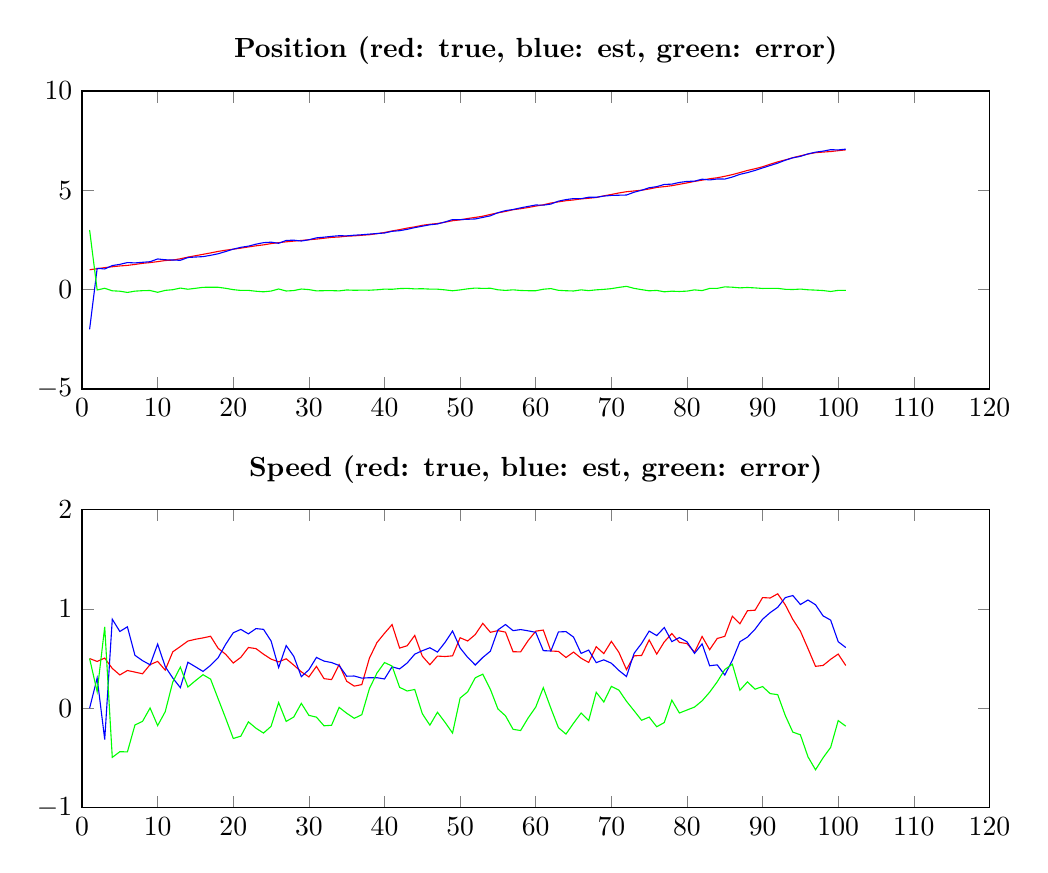
\begin{tikzpicture}

\begin{axis}[%
width=4.537in,
height=1.49in,
at={(0.761in,2.579in)},
scale only axis,
xmin=0,
xmax=120,
ymin=-5,
ymax=10,
axis background/.style={fill=white},
title style={font=\bfseries},
title={Position (red: true, blue: est, green: error)}
]
\addplot [color=red,solid,forget plot]
  table[row sep=crcr]{%
1	1\\
2	1.05350098526093\\
3	1.10635390818995\\
4	1.15146727243162\\
5	1.19128865650474\\
6	1.21969224676822\\
7	1.26704178742525\\
8	1.32278340016183\\
9	1.36070565004094\\
10	1.40827887277796\\
11	1.46417180017871\\
12	1.48639074171217\\
13	1.553080240981\\
14	1.63541515423249\\
15	1.70647088000168\\
16	1.77627177041997\\
17	1.84687871467326\\
18	1.92341334382681\\
19	1.98476955038119\\
20	2.03539278504865\\
21	2.08690337800104\\
22	2.14822136262328\\
23	2.20485114870535\\
24	2.25289847130034\\
25	2.31574047290658\\
26	2.36360913367107\\
27	2.40600854688746\\
28	2.44114551235687\\
29	2.47513056681039\\
30	2.5106764893933\\
31	2.54273557265424\\
32	2.58609728552767\\
33	2.62984263508844\\
34	2.64898752309515\\
35	2.68866600692662\\
36	2.70555380791937\\
37	2.73608141281007\\
38	2.76361798660698\\
39	2.8153481223731\\
40	2.87471906258833\\
41	2.95215979122992\\
42	3.02030866777573\\
43	3.09738939758793\\
44	3.15874293697989\\
45	3.23679507586606\\
46	3.28937601205318\\
47	3.32714162044263\\
48	3.39267621435652\\
49	3.46758613131786\\
50	3.5095911193115\\
51	3.57990028011702\\
52	3.63451457652295\\
53	3.69526629362559\\
54	3.78451039588291\\
55	3.86401375802301\\
56	3.9358814473823\\
57	4.02197126306334\\
58	4.07207567968295\\
59	4.1332352952039\\
60	4.20450999980021\\
61	4.26884014798831\\
62	4.35862130236071\\
63	4.41715972504581\\
64	4.47492794912828\\
65	4.51393557587917\\
66	4.56653612239395\\
67	4.59805905779586\\
68	4.63698731559741\\
69	4.72030952548425\\
70	4.78965144312392\\
71	4.8643633695578\\
72	4.92715752570044\\
73	4.96544316155725\\
74	5.00323567287665\\
75	5.06609005933895\\
76	5.14337622625101\\
77	5.18405546901296\\
78	5.23084958610435\\
79	5.30123400299849\\
80	5.37133903842606\\
81	5.44655560672986\\
82	5.50982980481865\\
83	5.58091967427126\\
84	5.63058224813438\\
85	5.70364344753136\\
86	5.78850585316195\\
87	5.89109041515268\\
88	5.99734797423989\\
89	6.08529448375654\\
90	6.18334091416315\\
91	6.31136602756521\\
92	6.43025330830646\\
93	6.52958972540131\\
94	6.63907856913582\\
95	6.73374736556153\\
96	6.82331058670917\\
97	6.89317700989917\\
98	6.92359788736719\\
99	6.95016142319149\\
100	6.9932296080585\\
101	7.03541326680543\\
};
\addplot [color=blue,solid,forget plot]
  table[row sep=crcr]{%
1	-2\\
2	1.07180465269847\\
3	1.03969611180212\\
4	1.21028915518896\\
5	1.27123695592158\\
6	1.3623376530376\\
7	1.34346937146479\\
8	1.37557965299266\\
9	1.40517970736248\\
10	1.54395491227077\\
11	1.50275246910858\\
12	1.49066464038814\\
13	1.47552564502242\\
14	1.61601168000405\\
15	1.64088996345228\\
16	1.66100086382625\\
17	1.72635994950759\\
18	1.80511493035112\\
19	1.91901351108413\\
20	2.03696127280667\\
21	2.12859743033884\\
22	2.18715882604155\\
23	2.28658891759857\\
24	2.36323791014358\\
25	2.38822252859795\\
26	2.33178368254894\\
27	2.47537791802108\\
28	2.48835009552842\\
29	2.44552361056464\\
30	2.5093245414563\\
31	2.60581105933807\\
32	2.63982325128122\\
33	2.68038537142895\\
34	2.71271279403409\\
35	2.70565510400454\\
36	2.73875067662153\\
37	2.76131744781897\\
38	2.79355682765893\\
39	2.82428176525007\\
40	2.84907333890794\\
41	2.93545287430367\\
42	2.96719937018645\\
43	3.03458021801721\\
44	3.12130304459239\\
45	3.1918288612483\\
46	3.26349896104264\\
47	3.30434370370896\\
48	3.4056293297775\\
49	3.52536333477245\\
50	3.52406772324543\\
51	3.54060547819677\\
52	3.55632268518552\\
53	3.63509886716404\\
54	3.71521045094579\\
55	3.87221995296429\\
56	3.97615265031005\\
57	4.03178889240971\\
58	4.11493369907814\\
59	4.18817250371029\\
60	4.25917801856492\\
61	4.24997316228391\\
62	4.30635013014211\\
63	4.45300115632272\\
64	4.53121691662921\\
65	4.58277783852822\\
66	4.5781032470713\\
67	4.64894324422776\\
68	4.64874373528728\\
69	4.70775710711303\\
70	4.74077052492485\\
71	4.75206183416066\\
72	4.76177567321951\\
73	4.90190292141689\\
74	5.00372709506768\\
75	5.12640592465942\\
76	5.18314120043615\\
77	5.29387695372061\\
78	5.30928691128357\\
79	5.39522920999918\\
80	5.44670515355324\\
81	5.45957884368007\\
82	5.55907675129664\\
83	5.52165299435891\\
84	5.56856145202528\\
85	5.56470955747292\\
86	5.6668811168972\\
87	5.80197273653683\\
88	5.89046624942459\\
89	5.998756313314\\
90	6.12515400060132\\
91	6.24546673724017\\
92	6.36660476155003\\
93	6.51357565631414\\
94	6.63457932820351\\
95	6.70596023228048\\
96	6.83158694911757\\
97	6.91828310488095\\
98	6.97043731843882\\
99	7.0436249212218\\
100	7.03147576992064\\
101	7.07117059986345\\
};
\addplot [color=green,solid,forget plot]
  table[row sep=crcr]{%
1	3\\
2	-0.0183036674375461\\
3	0.0666577963878268\\
4	-0.0588218827573495\\
5	-0.0799482994168401\\
6	-0.142645406269376\\
7	-0.0764275840395441\\
8	-0.0527962528308266\\
9	-0.0444740573215425\\
10	-0.135676039492809\\
11	-0.0385806689298644\\
12	-0.00427389867597006\\
13	0.0775545959585833\\
14	0.0194034742284359\\
15	0.0655809165494003\\
16	0.115270906593716\\
17	0.120518765165663\\
18	0.118298413475688\\
19	0.065756039297054\\
20	-0.00156848775802176\\
21	-0.0416940523378004\\
22	-0.0389374634182698\\
23	-0.0817377688932219\\
24	-0.110339438843233\\
25	-0.0724820556913652\\
26	0.0318254511221325\\
27	-0.0693693711336154\\
28	-0.0472045831715509\\
29	0.0296069562457495\\
30	0.00135194793699567\\
31	-0.0630754866838354\\
32	-0.0537259657535536\\
33	-0.0505427363405091\\
34	-0.0637252709389422\\
35	-0.0169890970779223\\
36	-0.0331968687021598\\
37	-0.0252360350088945\\
38	-0.0299388410519486\\
39	-0.00893364287697507\\
40	0.0256457236803844\\
41	0.016706916926251\\
42	0.053109297589284\\
43	0.0628091795707184\\
44	0.0374398923874963\\
45	0.0449662146177663\\
46	0.0258770510105406\\
47	0.0227979167336736\\
48	-0.0129531154209803\\
49	-0.0577772034545845\\
50	-0.0144766039339319\\
51	0.039294801920255\\
52	0.07819189133743\\
53	0.0601674264615535\\
54	0.0692999449371228\\
55	-0.00820619494127817\\
56	-0.0402712029277463\\
57	-0.00981762934637675\\
58	-0.0428580193951973\\
59	-0.0549372085063835\\
60	-0.0546680187647102\\
61	0.0188669857043999\\
62	0.0522711722185942\\
63	-0.0358414312769124\\
64	-0.0562889675009295\\
65	-0.0688422626490448\\
66	-0.011567124677355\\
67	-0.0508841864318983\\
68	-0.0117564196898696\\
69	0.0125524183712216\\
70	0.0488809181990613\\
71	0.112301535397145\\
72	0.165381852480936\\
73	0.0635402401403553\\
74	-0.000491422191028157\\
75	-0.0603158653204687\\
76	-0.0397649741851422\\
77	-0.109821484707647\\
78	-0.0784373251792214\\
79	-0.0939952070006891\\
80	-0.0753661151271787\\
81	-0.0130232369502146\\
82	-0.0492469464779894\\
83	0.0592666799123487\\
84	0.0620207961091088\\
85	0.138933890058441\\
86	0.121624736264754\\
87	0.0891176786158576\\
88	0.106881724815301\\
89	0.086538170442541\\
90	0.0581869135618263\\
91	0.0658992903250368\\
92	0.0636485467564318\\
93	0.0160140690871726\\
94	0.00449924093230436\\
95	0.027787133281044\\
96	-0.00827636240839702\\
97	-0.0251060949817807\\
98	-0.0468394310716276\\
99	-0.0934634980303128\\
100	-0.0382461618621468\\
101	-0.0357573330580134\\
};
\end{axis}

\begin{axis}[%
width=4.537in,
height=1.49in,
at={(0.761in,0.486in)},
scale only axis,
xmin=0,
xmax=120,
ymin=-1,
ymax=2,
axis background/.style={fill=white},
title style={font=\bfseries},
title={Speed (red: true, blue: est, green: error)}
]
\addplot [color=red,solid,forget plot]
  table[row sep=crcr]{%
1	0.5\\
2	0.4708692842533\\
3	0.504835010935357\\
4	0.400819235590837\\
5	0.335119315985957\\
6	0.379719778848935\\
7	0.363703510821044\\
8	0.346623630220598\\
9	0.439107296750358\\
10	0.471322387385188\\
11	0.38367338603834\\
12	0.567681435208591\\
13	0.621063214007748\\
14	0.67629280905186\\
15	0.694248957671398\\
16	0.707961287854704\\
17	0.72428595563249\\
18	0.603022846319019\\
19	0.542513240963362\\
20	0.455101723404011\\
21	0.512237792210319\\
22	0.611324863897447\\
23	0.600259236143207\\
24	0.54381984359013\\
25	0.494266223952595\\
26	0.466726416412408\\
27	0.497632455088684\\
28	0.434078299497699\\
29	0.366700989174428\\
30	0.314850043517129\\
31	0.421431759262248\\
32	0.297627671299819\\
33	0.288080337975726\\
34	0.438998965102491\\
35	0.271596551542958\\
36	0.222340801324222\\
37	0.237904057796335\\
38	0.503224274817569\\
39	0.661007775603718\\
40	0.754197121276001\\
41	0.841822157824901\\
42	0.605616970535387\\
43	0.62912425493669\\
44	0.732940726129104\\
45	0.523890544525107\\
46	0.437887810181254\\
47	0.524877988852534\\
48	0.520613566100879\\
49	0.527296304312277\\
50	0.709630767591188\\
51	0.676947134771206\\
52	0.741585431077125\\
53	0.854472633359159\\
54	0.764339470510461\\
55	0.78108513827331\\
56	0.766089046364991\\
57	0.568715288790155\\
58	0.567113189949712\\
59	0.681203021488086\\
60	0.775762174666498\\
61	0.786744326678224\\
62	0.575958152392863\\
63	0.572136172419703\\
64	0.51074715827293\\
65	0.565280211883044\\
66	0.503076019083728\\
67	0.460675178040698\\
68	0.619139145117133\\
69	0.549921333014754\\
70	0.673261449966055\\
71	0.561825326491251\\
72	0.388861125075395\\
73	0.527430195822526\\
74	0.531158505824533\\
75	0.687231891378543\\
76	0.544783589683091\\
77	0.668090679862609\\
78	0.751640379069887\\
79	0.66273023779175\\
80	0.650843501795715\\
81	0.563891752740356\\
82	0.722459045280547\\
83	0.58928207210652\\
84	0.702238823676071\\
85	0.723516755462026\\
86	0.925987257203682\\
87	0.850253887655056\\
88	0.981426423598619\\
89	0.986737902341994\\
90	1.11384881182123\\
91	1.10955282427791\\
92	1.15218007871592\\
93	1.04054201211802\\
94	0.893752414704328\\
95	0.776227983466876\\
96	0.600858237180188\\
97	0.421732508359978\\
98	0.430728716618293\\
99	0.492525582006519\\
100	0.54531312004684\\
101	0.429969130668949\\
};
\addplot [color=blue,solid,forget plot]
  table[row sep=crcr]{%
1	0\\
2	0.304138773397103\\
3	-0.314712533880966\\
4	0.895933426358408\\
5	0.772594903957269\\
6	0.819570883707619\\
7	0.532246582760038\\
8	0.479135357270411\\
9	0.436746525145716\\
10	0.646208921917506\\
11	0.418866568273422\\
12	0.303947511891543\\
13	0.207033679123882\\
14	0.46278341251766\\
15	0.416922163112348\\
16	0.370535696581441\\
17	0.431489625171616\\
18	0.508238726685386\\
19	0.644244206664443\\
20	0.759655571110965\\
21	0.793441375086613\\
22	0.748640760359272\\
23	0.801590109656971\\
24	0.794025289590206\\
25	0.676748834639319\\
26	0.40927573958342\\
27	0.630528015080319\\
28	0.522601242253264\\
29	0.31768287111247\\
30	0.386715786551563\\
31	0.51131199804418\\
32	0.47441898563138\\
33	0.459592428519742\\
34	0.430214593046898\\
35	0.322289398278464\\
36	0.324157071660509\\
37	0.302931712569086\\
38	0.307125969756631\\
39	0.307152564907545\\
40	0.294386489115254\\
41	0.41709928165308\\
42	0.395627178316378\\
43	0.455577780503936\\
44	0.544292207506892\\
45	0.578981837191058\\
46	0.608661570281662\\
47	0.565513599293321\\
48	0.661920016128981\\
49	0.777307908717157\\
50	0.606998815787617\\
51	0.511825411740996\\
52	0.43539438730568\\
53	0.511332777446421\\
54	0.5737836655383\\
55	0.788497834241158\\
56	0.842553797632273\\
57	0.780876950091079\\
58	0.791775486185352\\
59	0.778976952150322\\
60	0.764123675915349\\
61	0.579610762707277\\
62	0.57619686483938\\
63	0.768067508516545\\
64	0.771104052187206\\
65	0.716042589258848\\
66	0.551654721214255\\
67	0.585434749887859\\
68	0.458838270755759\\
69	0.48713363518568\\
70	0.453298822649899\\
71	0.379942598434862\\
72	0.318995716607752\\
73	0.552236214071748\\
74	0.652664647308222\\
75	0.776393521190276\\
76	0.73134333327966\\
77	0.812377817033345\\
78	0.670512862145589\\
79	0.711224714181449\\
80	0.668884657745796\\
81	0.552477897981123\\
82	0.6478409310157\\
83	0.427573707780745\\
84	0.436519677996718\\
85	0.334144529226882\\
86	0.482322354324987\\
87	0.669512236157427\\
88	0.715937831043218\\
89	0.795021657466291\\
90	0.896085776396022\\
91	0.962256034765884\\
92	1.01594457002903\\
93	1.11373492509581\\
94	1.13448883852248\\
95	1.04382851166263\\
96	1.08961097651528\\
97	1.04162799944157\\
98	0.929544760206228\\
99	0.886945348532681\\
100	0.669618022681749\\
101	0.610855214562555\\
};
\addplot [color=green,solid,forget plot]
  table[row sep=crcr]{%
1	0.5\\
2	0.166730510856198\\
3	0.819547544816323\\
4	-0.495114190767571\\
5	-0.437475587971312\\
6	-0.439851104858684\\
7	-0.168543071938994\\
8	-0.132511727049813\\
9	0.00236077160464254\\
10	-0.174886534532319\\
11	-0.0351931822350817\\
12	0.263733923317048\\
13	0.414029534883866\\
14	0.2135093965342\\
15	0.277326794559051\\
16	0.337425591273263\\
17	0.292796330460874\\
18	0.0947841196336329\\
19	-0.101730965701081\\
20	-0.304553847706954\\
21	-0.281203582876294\\
22	-0.137315896461825\\
23	-0.201330873513763\\
24	-0.250205446000077\\
25	-0.182482610686724\\
26	0.0574506768289882\\
27	-0.132895559991635\\
28	-0.0885229427555655\\
29	0.0490181180619585\\
30	-0.0718657430344347\\
31	-0.0898802387819323\\
32	-0.176791314331561\\
33	-0.171512090544016\\
34	0.00878437205559335\\
35	-0.0506928467355064\\
36	-0.101816270336287\\
37	-0.0650276547727503\\
38	0.196098305060938\\
39	0.353855210696173\\
40	0.459810632160747\\
41	0.42472287617182\\
42	0.209989792219009\\
43	0.173546474432753\\
44	0.188648518622212\\
45	-0.0550912926659501\\
46	-0.170773760100407\\
47	-0.0406356104407877\\
48	-0.141306450028102\\
49	-0.25001160440488\\
50	0.102631951803572\\
51	0.16512172303021\\
52	0.306191043771445\\
53	0.343139855912738\\
54	0.190555804972161\\
55	-0.00741269596784844\\
56	-0.0764647512672818\\
57	-0.212161661300924\\
58	-0.22466229623564\\
59	-0.0977739306622359\\
60	0.0116384987511491\\
61	0.207133563970947\\
62	-0.000238712446517186\\
63	-0.195931336096843\\
64	-0.260356893914276\\
65	-0.150762377375805\\
66	-0.0485787021305273\\
67	-0.124759571847161\\
68	0.160300874361374\\
69	0.0627876978290741\\
70	0.219962627316157\\
71	0.181882728056389\\
72	0.0698654084676432\\
73	-0.0248060182492218\\
74	-0.121506141483689\\
75	-0.0891616298117335\\
76	-0.186559743596569\\
77	-0.144287137170736\\
78	0.0811275169242984\\
79	-0.0484944763896996\\
80	-0.0180411559500812\\
81	0.0114138547592335\\
82	0.074618114264847\\
83	0.161708364325775\\
84	0.265719145679353\\
85	0.389372226235144\\
86	0.443664902878695\\
87	0.180741651497628\\
88	0.265488592555401\\
89	0.191716244875703\\
90	0.217763035425204\\
91	0.147296789512029\\
92	0.136235508686888\\
93	-0.073192912977794\\
94	-0.240736423818154\\
95	-0.267600528195756\\
96	-0.48875273933509\\
97	-0.619895491081589\\
98	-0.498816043587935\\
99	-0.394419766526163\\
100	-0.124304902634909\\
101	-0.180886083893606\\
};
\end{axis}
\end{tikzpicture}%}
	\scalebox{0.5}{% This file was created by matlab2tikz.
%
%The latest updates can be retrieved from
%  http://www.mathworks.com/matlabcentral/fileexchange/22022-matlab2tikz-matlab2tikz
%where you can also make suggestions and rate matlab2tikz.
%
\definecolor{mycolor1}{rgb}{0.00000,0.44700,0.74100}%
%
\begin{tikzpicture}

\begin{axis}[%
width=4.521in,
height=1.474in,
at={(0.758in,2.554in)},
scale only axis,
xmin=0,
xmax=120,
ymin=0,
ymax=1,
axis background/.style={fill=white},
title style={font=\bfseries},
title={sqrt(P(1,1))}
]
\addplot [color=mycolor1,solid,forget plot]
  table[row sep=crcr]{%
1	1\\
2	0.00999950498775105\\
3	0.0099503963723716\\
4	0.00911943030315727\\
5	0.00837714153091052\\
6	0.00778136666909862\\
7	0.00731091510653059\\
8	0.00694357189595119\\
9	0.00666237665582672\\
10	0.00645379129685296\\
11	0.00630563089180991\\
12	0.00620599915171016\\
13	0.00614327106056545\\
14	0.00610673343204126\\
15	0.00608734397009586\\
16	0.00607819191174998\\
17	0.00607451730841707\\
18	0.00607338253816797\\
19	0.00607318631676735\\
20	0.006073186082685\\
21	0.00607312032613669\\
22	0.00607295442725656\\
23	0.00607273335922854\\
24	0.00607251009111614\\
25	0.00607231960260479\\
26	0.00607217595180164\\
27	0.0060720782058555\\
28	0.00607201773622705\\
29	0.00607198379318334\\
30	0.00607196671963812\\
31	0.00607195924360212\\
32	0.00607195657184777\\
33	0.00607195591504189\\
34	0.00607195586406135\\
35	0.00607195583803307\\
36	0.00607195568371097\\
37	0.00607195542585966\\
38	0.00607195513424207\\
39	0.00607195486648328\\
40	0.00607195465295048\\
41	0.00607195450051336\\
42	0.00607195440181207\\
43	0.00607195434370278\\
44	0.00607195431281447\\
45	0.00607195429828058\\
46	0.00607195429248435\\
47	0.0060719542907171\\
48	0.00607195429042213\\
49	0.0060719542904221\\
50	0.00607195429030827\\
51	0.00607195429003183\\
52	0.00607195428966829\\
53	0.00607195428930377\\
54	0.00607195428899431\\
55	0.00607195428876186\\
56	0.00607195428860424\\
57	0.00607195428850707\\
58	0.00607195428845273\\
59	0.00607195428842552\\
60	0.00607195428841368\\
61	0.00607195428840949\\
62	0.00607195428840848\\
63	0.0060719542884084\\
64	0.00607195428840836\\
65	0.00607195428840809\\
66	0.00607195428840767\\
67	0.00607195428840719\\
68	0.00607195428840675\\
69	0.00607195428840641\\
70	0.00607195428840616\\
71	0.006071954288406\\
72	0.00607195428840591\\
73	0.00607195428840586\\
74	0.00607195428840584\\
75	0.00607195428840583\\
76	0.00607195428840583\\
77	0.00607195428840583\\
78	0.00607195428840583\\
79	0.00607195428840583\\
80	0.00607195428840582\\
81	0.00607195428840582\\
82	0.00607195428840582\\
83	0.00607195428840582\\
84	0.00607195428840582\\
85	0.00607195428840582\\
86	0.00607195428840582\\
87	0.00607195428840582\\
88	0.00607195428840582\\
89	0.00607195428840582\\
90	0.00607195428840582\\
91	0.00607195428840582\\
92	0.00607195428840582\\
93	0.00607195428840582\\
94	0.00607195428840582\\
95	0.00607195428840582\\
96	0.00607195428840582\\
97	0.00607195428840582\\
98	0.00607195428840582\\
99	0.00607195428840582\\
100	0.00607195428840582\\
101	0.00607195428840582\\
};
\end{axis}

\begin{axis}[%
width=4.521in,
height=1.474in,
at={(0.758in,0.481in)},
scale only axis,
xmin=0,
xmax=120,
ymin=0,
ymax=1,
axis background/.style={fill=white},
title style={font=\bfseries},
title={sqrt(P(2,2))}
]
\addplot [color=mycolor1,solid,forget plot]
  table[row sep=crcr]{%
1	1\\
2	0.995087935762966\\
3	0.140695729370425\\
4	0.0717554496392457\\
5	0.0467710194564084\\
6	0.0348862867353259\\
7	0.0286123242340356\\
8	0.0251924258529208\\
9	0.0233421318139014\\
10	0.0223745061660255\\
11	0.0218973386309799\\
12	0.0216824318593398\\
13	0.0215985208565236\\
14	0.0215730114143649\\
15	0.0215686455648599\\
16	0.0215686411604006\\
17	0.0215671602575261\\
18	0.0215634391861115\\
19	0.0215584868711597\\
20	0.0215534888967884\\
21	0.0215492273662283\\
22	0.021546015619212\\
23	0.0215438315223552\\
24	0.0215424811535395\\
25	0.0215417236226275\\
26	0.0215413428405024\\
27	0.0215411762517794\\
28	0.0215411167971786\\
29	0.0215411022226114\\
30	0.0215411011058976\\
31	0.0215411005120385\\
32	0.0215410970423779\\
33	0.0215410912621791\\
34	0.0215410847339378\\
35	0.021541078744862\\
36	0.0215410739716557\\
37	0.0215410705659281\\
38	0.021541068361826\\
39	0.021541067064828\\
40	0.0215410663757871\\
41	0.0215410660518011\\
42	0.0215410659227257\\
43	0.0215410658834443\\
44	0.0215410658769221\\
45	0.0215410658769217\\
46	0.0215410658743538\\
47	0.0215410658681502\\
48	0.0215410658600073\\
49	0.021541065851851\\
50	0.0215410658449314\\
51	0.0215410658397367\\
52	0.0215410658362162\\
53	0.0215410658340469\\
54	0.0215410658328344\\
55	0.0215410658322275\\
56	0.0215410658319637\\
57	0.0215410658318704\\
58	0.021541065831848\\
59	0.0215410658318464\\
60	0.0215410658318453\\
61	0.0215410658318394\\
62	0.0215410658318299\\
63	0.0215410658318192\\
64	0.0215410658318094\\
65	0.0215410658318017\\
66	0.0215410658317962\\
67	0.0215410658317927\\
68	0.0215410658317906\\
69	0.0215410658317895\\
70	0.021541065831789\\
71	0.0215410658317888\\
72	0.0215410658317887\\
73	0.0215410658317887\\
74	0.0215410658317887\\
75	0.0215410658317887\\
76	0.0215410658317887\\
77	0.0215410658317887\\
78	0.0215410658317886\\
79	0.0215410658317886\\
80	0.0215410658317886\\
81	0.0215410658317886\\
82	0.0215410658317886\\
83	0.0215410658317886\\
84	0.0215410658317886\\
85	0.0215410658317886\\
86	0.0215410658317886\\
87	0.0215410658317886\\
88	0.0215410658317886\\
89	0.0215410658317886\\
90	0.0215410658317886\\
91	0.0215410658317886\\
92	0.0215410658317886\\
93	0.0215410658317886\\
94	0.0215410658317886\\
95	0.0215410658317886\\
96	0.0215410658317886\\
97	0.0215410658317886\\
98	0.0215410658317886\\
99	0.0215410658317886\\
100	0.0215410658317886\\
101	0.0215410658317886\\
};
\end{axis}
\end{tikzpicture}%}
	\scalebox{0.5}{% This file was created by matlab2tikz.
%
%The latest updates can be retrieved from
%  http://www.mathworks.com/matlabcentral/fileexchange/22022-matlab2tikz-matlab2tikz
%where you can also make suggestions and rate matlab2tikz.
%
\definecolor{mycolor1}{rgb}{0.00000,0.44700,0.74100}%
%
\begin{tikzpicture}

\begin{axis}[%
width=4.521in,
height=1.474in,
at={(0.758in,2.554in)},
scale only axis,
xmin=0,
xmax=100,
ymin=0.2,
ymax=1,
axis background/.style={fill=white},
title style={font=\bfseries},
title={K(1)}
]
\addplot [color=mycolor1,solid,forget plot]
  table[row sep=crcr]{%
1	0.99990099999901\\
2	0.990103879673073\\
3	0.83164009054143\\
4	0.701765002289058\\
5	0.605496672389589\\
6	0.534494796948972\\
7	0.482131906742431\\
8	0.443872627041049\\
9	0.41651422103335\\
10	0.397609809437474\\
11	0.385144254710273\\
12	0.37739779323581\\
13	0.372921932100104\\
14	0.370557566102624\\
15	0.369444169160629\\
16	0.368997605302586\\
17	0.368859754549237\\
18	0.368835920381702\\
19	0.368835891949188\\
20	0.368827904957346\\
21	0.36880775475535\\
22	0.368780904522871\\
23	0.368753788067073\\
24	0.368730653561784\\
25	0.368713207896382\\
26	0.368701337380253\\
27	0.368693993890559\\
28	0.368689871846811\\
29	0.368687798443929\\
30	0.368686890559652\\
31	0.368686566104053\\
32	0.368686486342121\\
33	0.36868648015109\\
34	0.368686476990238\\
35	0.368686458249499\\
36	0.368686426936266\\
37	0.368686391522486\\
38	0.3686863590061\\
39	0.36868633307487\\
40	0.368686314563045\\
41	0.368686302576849\\
42	0.36868629552011\\
43	0.368686291769063\\
44	0.368686290004081\\
45	0.368686289300191\\
46	0.368686289085577\\
47	0.368686289049757\\
48	0.368686289049753\\
49	0.368686289035931\\
50	0.36868628900236\\
51	0.368686288958212\\
52	0.368686288913945\\
53	0.368686288876364\\
54	0.368686288848135\\
55	0.368686288828995\\
56	0.368686288817194\\
57	0.368686288810595\\
58	0.368686288807291\\
59	0.368686288805852\\
60	0.368686288805343\\
61	0.368686288805221\\
62	0.368686288805212\\
63	0.368686288805206\\
64	0.368686288805175\\
65	0.368686288805123\\
66	0.368686288805065\\
67	0.368686288805012\\
68	0.36868628880497\\
69	0.36868628880494\\
70	0.36868628880492\\
71	0.368686288804909\\
72	0.368686288804903\\
73	0.3686862888049\\
74	0.368686288804899\\
75	0.368686288804899\\
76	0.368686288804899\\
77	0.368686288804899\\
78	0.368686288804899\\
79	0.368686288804899\\
80	0.368686288804899\\
81	0.368686288804899\\
82	0.368686288804899\\
83	0.368686288804899\\
84	0.368686288804899\\
85	0.368686288804899\\
86	0.368686288804899\\
87	0.368686288804899\\
88	0.368686288804899\\
89	0.368686288804899\\
90	0.368686288804899\\
91	0.368686288804899\\
92	0.368686288804899\\
93	0.368686288804899\\
94	0.368686288804899\\
95	0.368686288804899\\
96	0.368686288804899\\
97	0.368686288804899\\
98	0.368686288804899\\
99	0.368686288804899\\
100	0.368686288804899\\
};
\end{axis}

\begin{axis}[%
width=4.521in,
height=1.474in,
at={(0.758in,0.481in)},
scale only axis,
xmin=0,
xmax=100,
ymin=0,
ymax=10,
axis background/.style={fill=white},
title style={font=\bfseries},
title={K(2)}
]
\addplot [color=mycolor1,solid,forget plot]
  table[row sep=crcr]{%
1	0.09900000099\\
2	9.80011806266567\\
3	4.98267992939143\\
4	3.02157518079358\\
5	2.05500864165115\\
6	1.52316171990681\\
7	1.21275738896694\\
8	1.02739844518826\\
9	0.917387594826839\\
10	0.854192977448231\\
11	0.820024755641724\\
12	0.803251860166227\\
13	0.796231099581053\\
14	0.794120890423405\\
15	0.794076210997973\\
16	0.794610268370614\\
17	0.795080609315982\\
18	0.795306199970914\\
19	0.795313833306704\\
20	0.795192715199651\\
21	0.7950257133309\\
22	0.794866750414977\\
23	0.794741144153941\\
24	0.79465425041923\\
25	0.794600752801905\\
26	0.794571564627845\\
27	0.794557849773942\\
28	0.794552762363279\\
29	0.794551763753304\\
30	0.794552245582542\\
31	0.794552941966156\\
32	0.794553387619492\\
33	0.794553519546352\\
34	0.794553429254262\\
35	0.79455323294521\\
36	0.794553018599259\\
37	0.794552835220353\\
38	0.794552700426997\\
39	0.794552612690195\\
40	0.794552561858415\\
41	0.794552536041202\\
42	0.794552525113207\\
43	0.794552521866782\\
44	0.79455252186123\\
45	0.794552522743607\\
46	0.794552523500928\\
47	0.794552523855391\\
48	0.794552523857701\\
49	0.794552523654715\\
50	0.794552523380618\\
51	0.794552523121854\\
52	0.794552522918453\\
53	0.79455252277834\\
54	0.794552522692434\\
55	0.794552522645785\\
56	0.794552522624009\\
57	0.794552522616029\\
58	0.794552522614542\\
59	0.794552522615371\\
60	0.794552522616505\\
61	0.794552522617215\\
62	0.794552522617415\\
63	0.794552522617257\\
64	0.794552522616932\\
65	0.794552522616582\\
66	0.794552522616284\\
67	0.794552522616066\\
68	0.794552522615925\\
69	0.794552522615843\\
70	0.794552522615802\\
71	0.794552522615785\\
72	0.79455252261578\\
73	0.79455252261578\\
74	0.794552522615781\\
75	0.794552522615783\\
76	0.794552522615783\\
77	0.794552522615783\\
78	0.794552522615783\\
79	0.794552522615782\\
80	0.794552522615782\\
81	0.794552522615782\\
82	0.794552522615781\\
83	0.794552522615781\\
84	0.794552522615781\\
85	0.794552522615781\\
86	0.794552522615781\\
87	0.794552522615781\\
88	0.794552522615781\\
89	0.794552522615781\\
90	0.794552522615781\\
91	0.794552522615781\\
92	0.794552522615781\\
93	0.794552522615781\\
94	0.794552522615781\\
95	0.794552522615781\\
96	0.794552522615781\\
97	0.794552522615781\\
98	0.794552522615781\\
99	0.794552522615781\\
100	0.794552522615781\\
};
\end{axis}
\end{tikzpicture}%}

	\caption{$Q / 100, R / 100$}
	\label{fig:q3:Q-R-100}
\end{figure}


\begin{figure}[H]
	\scalebox{0.5}{% This file was created by matlab2tikz.
%
%The latest updates can be retrieved from
%  http://www.mathworks.com/matlabcentral/fileexchange/22022-matlab2tikz-matlab2tikz
%where you can also make suggestions and rate matlab2tikz.
%
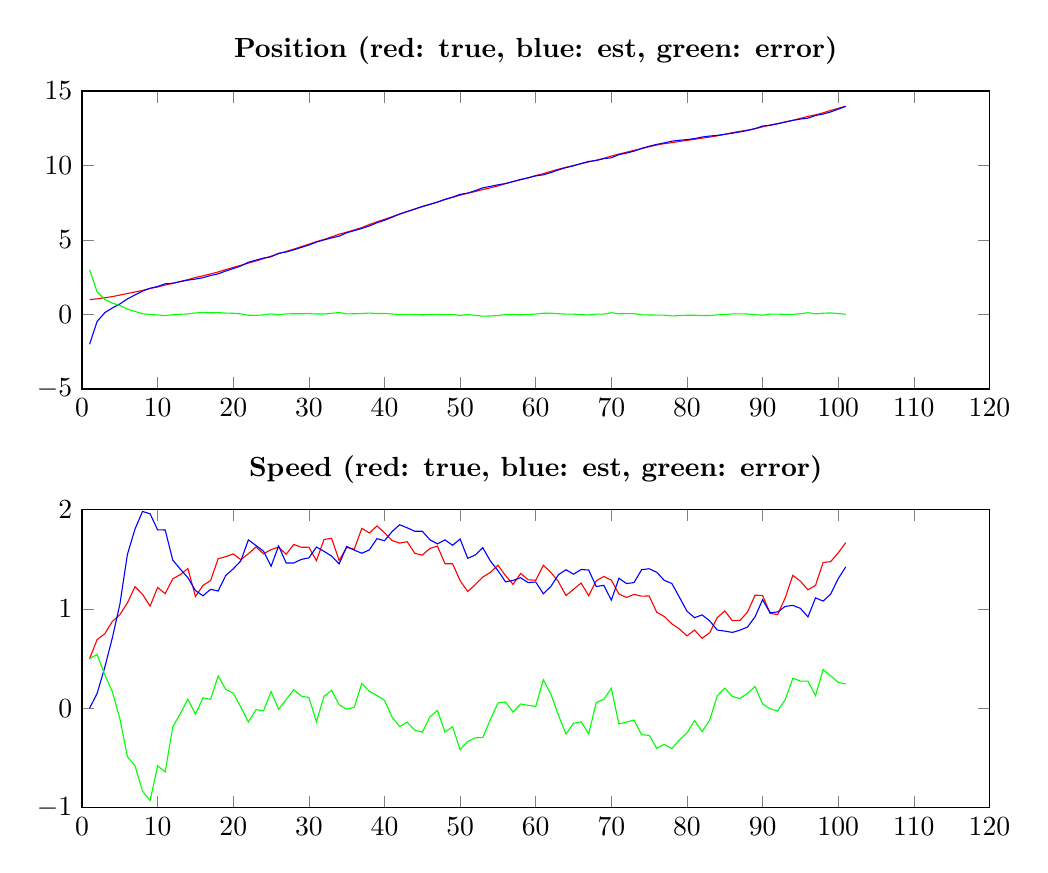
\begin{tikzpicture}

\begin{axis}[%
width=4.537in,
height=1.49in,
at={(0.761in,2.579in)},
scale only axis,
xmin=0,
xmax=120,
ymin=-5,
ymax=15,
axis background/.style={fill=white},
title style={font=\bfseries},
title={Position (red: true, blue: est, green: error)}
]
\addplot [color=red,solid,forget plot]
  table[row sep=crcr]{%
1	1\\
2	1.04475805241441\\
3	1.11948939053026\\
4	1.19626003080298\\
5	1.29990728100774\\
6	1.40516670408687\\
7	1.50694703767187\\
8	1.61468947205662\\
9	1.74723460470147\\
10	1.8434509842545\\
11	1.97834742048087\\
12	2.08044053121518\\
13	2.21400409247651\\
14	2.33888796365736\\
15	2.47924752919697\\
16	2.59124427069069\\
17	2.72165476557092\\
18	2.84998257416719\\
19	3.00526375436819\\
20	3.15776064160793\\
21	3.29619562986488\\
22	3.44831291310932\\
23	3.58733759203129\\
24	3.74932780768543\\
25	3.91157014398271\\
26	4.08033311532889\\
27	4.2314053339829\\
28	4.38641704464265\\
29	4.54615306145472\\
30	4.71836865499421\\
31	4.88685478051833\\
32	5.03328479928154\\
33	5.20740938500133\\
34	5.3872319686846\\
35	5.52294052229544\\
36	5.6722873899984\\
37	5.83468300257723\\
38	6.03524752946634\\
39	6.21776775491868\\
40	6.38660835412751\\
41	6.55808526339129\\
42	6.73698179007589\\
43	6.91084504608452\\
44	7.07303164421153\\
45	7.23060851208697\\
46	7.38518564298858\\
47	7.54481953897013\\
48	7.71086262643945\\
49	7.86097497731528\\
50	8.00212731187277\\
51	8.13691953910694\\
52	8.25062970786062\\
53	8.38034671970354\\
54	8.49535487046011\\
55	8.62461247805562\\
56	8.78052761907424\\
57	8.91843566588183\\
58	9.0391152036216\\
59	9.17071052659402\\
60	9.32392761936556\\
61	9.45073451692636\\
62	9.60580464039513\\
63	9.74933127265526\\
64	9.87597392147563\\
65	9.99517782562034\\
66	10.1147950489809\\
67	10.2369034667016\\
68	10.3533632987454\\
69	10.4780892126701\\
70	10.6309879988996\\
71	10.7672255699451\\
72	10.886212603691\\
73	11.0162931756113\\
74	11.1239468448786\\
75	11.2558528573006\\
76	11.3721570115024\\
77	11.4637574096275\\
78	11.5271524042988\\
79	11.613318007366\\
80	11.6823167040279\\
81	11.7532801789489\\
82	11.8311869011045\\
83	11.903890867604\\
84	11.9879776425322\\
85	12.0845381805487\\
86	12.2015855248513\\
87	12.2905062769501\\
88	12.3741130045726\\
89	12.4626950220253\\
90	12.5913614728659\\
91	12.7140687972289\\
92	12.8153346697957\\
93	12.920350052186\\
94	13.0329129450734\\
95	13.1622063406474\\
96	13.2908716828744\\
97	13.3972626359545\\
98	13.5328905015056\\
99	13.693266323802\\
100	13.8365498092199\\
101	13.9749315517448\\
};
\addplot [color=blue,solid,forget plot]
  table[row sep=crcr]{%
1	-2\\
2	-0.466138416734871\\
3	0.115905856417391\\
4	0.431888014891896\\
5	0.700960472010464\\
6	1.04270235941819\\
7	1.30897342824304\\
8	1.56618802226051\\
9	1.75400431033381\\
10	1.87705793037144\\
11	2.05635953421357\\
12	2.0958634140866\\
13	2.20296042776875\\
14	2.30309029166991\\
15	2.37416461115891\\
16	2.46815455768143\\
17	2.61138044807261\\
18	2.72325807818894\\
19	2.91356134104864\\
20	3.07863920323573\\
21	3.2560940985595\\
22	3.50249342647072\\
23	3.64577989509788\\
24	3.7826874096986\\
25	3.87077342418591\\
26	4.10812569004813\\
27	4.19206997324645\\
28	4.33836164323562\\
29	4.50136240397742\\
30	4.65816804968729\\
31	4.86009379718024\\
32	5.0024503532098\\
33	5.13788820198305\\
34	5.25472293859275\\
35	5.48160988184759\\
36	5.62732499174641\\
37	5.77194260840275\\
38	5.94349275362313\\
39	6.1555489820906\\
40	6.31652169441839\\
41	6.52773909680803\\
42	6.73757017744824\\
43	6.90801446763764\\
44	7.07343827741981\\
45	7.25188151730763\\
46	7.39028722854929\\
47	7.54048445235527\\
48	7.72465294407024\\
49	7.86889382885898\\
50	8.06197247105933\\
51	8.14265041936817\\
52	8.30847728688509\\
53	8.49701215057203\\
54	8.59641013579635\\
55	8.70015496539883\\
56	8.78604281534313\\
57	8.91965555782291\\
58	9.06099625011176\\
59	9.16944799347196\\
60	9.29874614718825\\
61	9.37112159523236\\
62	9.5203333216572\\
63	9.69784235453819\\
64	9.85546572382223\\
65	9.97412479125613\\
66	10.1308469042416\\
67	10.2681538103591\\
68	10.3301207086802\\
69	10.4582721272768\\
70	10.5129080541979\\
71	10.7238572473807\\
72	10.8301828548494\\
73	10.9600324030424\\
74	11.1466326621128\\
75	11.2906774583094\\
76	11.4145478229313\\
77	11.5135309804326\\
78	11.6276828710724\\
79	11.6890898539563\\
80	11.7356397203843\\
81	11.8030400627008\\
82	11.9070492420553\\
83	11.9732691582632\\
84	12.0183075835125\\
85	12.0920925864307\\
86	12.1635582333254\\
87	12.2503274355771\\
88	12.3433397100111\\
89	12.47254078873\\
90	12.6450138217608\\
91	12.6928142109663\\
92	12.7933098482773\\
93	12.9158056489523\\
94	13.0232909785513\\
95	13.112766868896\\
96	13.1733803997854\\
97	13.3541918377562\\
98	13.4502387953596\\
99	13.5906755932289\\
100	13.7777984044307\\
101	13.9632515543937\\
};
\addplot [color=green,solid,forget plot]
  table[row sep=crcr]{%
1	3\\
2	1.51089646914928\\
3	1.00358353411287\\
4	0.764372015911084\\
5	0.598946808997281\\
6	0.362464344668687\\
7	0.19797360942883\\
8	0.0485014497961158\\
9	-0.00676970563234058\\
10	-0.0336069461169384\\
11	-0.0780121137327059\\
12	-0.0154228828714205\\
13	0.0110436647077603\\
14	0.0357976719874467\\
15	0.105082918038059\\
16	0.123089713009267\\
17	0.110274317498317\\
18	0.126724495978255\\
19	0.0917024133195516\\
20	0.0791214383721939\\
21	0.0401015313053819\\
22	-0.0541805133614042\\
23	-0.0584423030665882\\
24	-0.0333596020131726\\
25	0.0407967197967927\\
26	-0.0277925747192365\\
27	0.0393353607364517\\
28	0.04805540140703\\
29	0.0447906574772992\\
30	0.0602006053069148\\
31	0.0267609833380877\\
32	0.0308344460717462\\
33	0.0695211830182823\\
34	0.132509030091856\\
35	0.0413306404478462\\
36	0.0449623982519967\\
37	0.0627403941744777\\
38	0.0917547758432082\\
39	0.0622187728280821\\
40	0.070086659709113\\
41	0.0303461665832572\\
42	-0.00058838737234268\\
43	0.0028305784468774\\
44	-0.000406633208280383\\
45	-0.0212730052206576\\
46	-0.00510158556070017\\
47	0.0043350866148586\\
48	-0.0137903176307921\\
49	-0.00791885154370231\\
50	-0.0598451591865619\\
51	-0.00573088026123081\\
52	-0.0578475790244646\\
53	-0.116665430868485\\
54	-0.101055265336242\\
55	-0.0755424873432116\\
56	-0.00551519626888641\\
57	-0.00121989194107641\\
58	-0.0218810464901562\\
59	0.00126253312206259\\
60	0.0251814721773034\\
61	0.079612921694002\\
62	0.0854713187379303\\
63	0.0514889181170677\\
64	0.0205081976534061\\
65	0.0210530343642077\\
66	-0.0160518552607467\\
67	-0.0312503436575966\\
68	0.0232425900652018\\
69	0.0198170853933135\\
70	0.118079944701739\\
71	0.0433683225644348\\
72	0.0560297488415564\\
73	0.0562607725688657\\
74	-0.0226858172342048\\
75	-0.0348246010087934\\
76	-0.042390811428934\\
77	-0.0497735708050797\\
78	-0.100530466773618\\
79	-0.0757718465902961\\
80	-0.0533230163563712\\
81	-0.0497598837518396\\
82	-0.0758623409508239\\
83	-0.0693782906591451\\
84	-0.0303299409802413\\
85	-0.00755440588203982\\
86	0.0380272915258342\\
87	0.0401788413730095\\
88	0.0307732945615538\\
89	-0.00984576670466453\\
90	-0.0536523488948593\\
91	0.0212545862625859\\
92	0.0220248215184089\\
93	0.00454440323370164\\
94	0.00962196652210956\\
95	0.0494394717513789\\
96	0.117491283088945\\
97	0.0430707981983698\\
98	0.0826517061460397\\
99	0.102590730573077\\
100	0.0587514047892093\\
101	0.0116799973510791\\
};
\end{axis}

\begin{axis}[%
width=4.537in,
height=1.49in,
at={(0.761in,0.486in)},
scale only axis,
xmin=0,
xmax=120,
ymin=-1,
ymax=2,
axis background/.style={fill=white},
title style={font=\bfseries},
title={Speed (red: true, blue: est, green: error)}
]
\addplot [color=red,solid,forget plot]
  table[row sep=crcr]{%
1	0.5\\
2	0.691129844549583\\
3	0.748537015102099\\
4	0.872945532788763\\
5	0.941578500753729\\
6	1.05983487759842\\
7	1.22377265072176\\
8	1.14615555247202\\
9	1.0278403763157\\
10	1.21581379024732\\
11	1.15335647714987\\
12	1.30338414234598\\
13	1.34548458714423\\
14	1.40641940721456\\
15	1.12444272778972\\
16	1.23623822721618\\
17	1.28567055198138\\
18	1.50480185297085\\
19	1.52555692067928\\
20	1.55369582889061\\
21	1.49529421038111\\
22	1.55565985215957\\
23	1.62370090174634\\
24	1.55438717857592\\
25	1.59700863825713\\
26	1.62196005257071\\
27	1.54975587524389\\
28	1.64927030425434\\
29	1.61980433013164\\
30	1.62139380378413\\
31	1.4849499990232\\
32	1.69888663299426\\
33	1.71067316783599\\
34	1.48804500232649\\
35	1.61860731267953\\
36	1.60063193361899\\
37	1.81076641408097\\
38	1.76423919567387\\
39	1.83515159726992\\
40	1.7660198662997\\
41	1.68781121726878\\
42	1.66274448050863\\
43	1.67612874647494\\
44	1.55981829125784\\
45	1.54114747899751\\
46	1.60817997563376\\
47	1.63238643402232\\
48	1.45494121980304\\
49	1.45482247114784\\
50	1.28434506076536\\
51	1.17562662901031\\
52	1.24371029476699\\
53	1.32051275167876\\
54	1.36746357410627\\
55	1.43913997827664\\
56	1.33573826438858\\
57	1.24698586644601\\
58	1.35665369876707\\
59	1.29278468206661\\
60	1.28782238070203\\
61	1.43945398335576\\
62	1.36752588068258\\
63	1.27388079854213\\
64	1.13400006985653\\
65	1.1977859962369\\
66	1.26001825277042\\
67	1.13285147394932\\
68	1.28268830154197\\
69	1.32611106375721\\
70	1.28938987591898\\
71	1.14948779999114\\
72	1.11507117721484\\
73	1.14602502247588\\
74	1.12798576231421\\
75	1.13070505841037\\
76	0.965808255007539\\
77	0.923030952506555\\
78	0.849576746420529\\
79	0.797986181755547\\
80	0.728247290556201\\
81	0.787043352388832\\
82	0.703491873834526\\
83	0.760096648004661\\
84	0.911349322059999\\
85	0.979279311301517\\
86	0.881417725832465\\
87	0.884037826143943\\
88	0.966496557540508\\
89	1.13778033768968\\
90	1.13510553278729\\
91	0.95429566411726\\
92	0.942676868268626\\
93	1.11289577160236\\
94	1.33798887397594\\
95	1.27848391608309\\
96	1.19239821978768\\
97	1.23601843635207\\
98	1.46730479953221\\
99	1.47547282178632\\
100	1.56443528529063\\
101	1.66690492516399\\
};
\addplot [color=blue,solid,forget plot]
  table[row sep=crcr]{%
1	0\\
2	0.150378586594621\\
3	0.409537356689921\\
4	0.705448008206124\\
5	1.04494934986831\\
6	1.54795542181511\\
7	1.80306280144229\\
8	1.98096181311864\\
9	1.95752560388123\\
10	1.79506294761913\\
11	1.79461324952196\\
12	1.49069168089363\\
13	1.40014554635165\\
14	1.31435135475888\\
15	1.1846009307113\\
16	1.13198079167617\\
17	1.19659735462659\\
18	1.17984013162666\\
19	1.33563874646378\\
20	1.40354880002371\\
21	1.4835067889003\\
22	1.69482966941857\\
23	1.63836912740463\\
24	1.5803303762786\\
25	1.42958292254291\\
26	1.63301383291565\\
27	1.46199124973506\\
28	1.4621906924578\\
29	1.49835665351043\\
30	1.51337754884092\\
31	1.62239902320212\\
32	1.57954866331688\\
33	1.53102247502661\\
34	1.45286270604293\\
35	1.62871958621814\\
36	1.59174501125288\\
37	1.56037359613763\\
38	1.59380506468425\\
39	1.70732604861535\\
40	1.68629259087715\\
41	1.77807391860807\\
42	1.84708788390186\\
43	1.81634659154131\\
44	1.78141073523386\\
45	1.78206193126027\\
46	1.69628826902442\\
47	1.65441139508822\\
48	1.69477054426386\\
49	1.64038430085529\\
50	1.70296860218625\\
51	1.50983168686072\\
52	1.54182120941883\\
53	1.61585449798497\\
54	1.48183484942302\\
55	1.3860655008604\\
56	1.27245190182277\\
57	1.28617455681289\\
58	1.31359429019949\\
59	1.26422614177403\\
60	1.27042319130876\\
61	1.15261110649758\\
62	1.22577777482111\\
63	1.34415963189827\\
64	1.39417370515089\\
65	1.34943767189117\\
66	1.39637199008074\\
67	1.3913499967199\\
68	1.22504571186937\\
69	1.23721518220353\\
70	1.08832944245658\\
71	1.30839925697583\\
72	1.25556866907388\\
73	1.26481978810887\\
74	1.39438015605834\\
75	1.40430818769579\\
76	1.36861890111731\\
77	1.28698678334395\\
78	1.25563713132365\\
79	1.11737353593216\\
80	0.976888565531006\\
81	0.911614059470544\\
82	0.93930218100065\\
83	0.879583957298195\\
84	0.787087512891652\\
85	0.776476386826876\\
86	0.763153631630794\\
87	0.785682606727042\\
88	0.816810771563173\\
89	0.919220701801334\\
90	1.09281536120569\\
91	0.960317891519407\\
92	0.969937890751825\\
93	1.02489704780135\\
94	1.03566307415599\\
95	1.00529694238402\\
96	0.919273975853661\\
97	1.11082717610255\\
98	1.07842374422657\\
99	1.14866769459624\\
100	1.30438604372864\\
101	1.42294739875198\\
};
\addplot [color=green,solid,forget plot]
  table[row sep=crcr]{%
1	0.5\\
2	0.540751257954962\\
3	0.338999658412178\\
4	0.167497524582639\\
5	-0.103370849114583\\
6	-0.48812054421669\\
7	-0.579290150720527\\
8	-0.834806260646624\\
9	-0.929685227565527\\
10	-0.579249157371815\\
11	-0.641256772372089\\
12	-0.187307538547652\\
13	-0.0546609592074174\\
14	0.0920680524556756\\
15	-0.0601582029215746\\
16	0.104257435540008\\
17	0.0890731973547885\\
18	0.32496172134419\\
19	0.189918174215505\\
20	0.150147028866902\\
21	0.0117874214808067\\
22	-0.139169817259001\\
23	-0.0146682256582948\\
24	-0.0259431977026718\\
25	0.16742571571422\\
26	-0.0110537803449342\\
27	0.0877646255088271\\
28	0.187079611796534\\
29	0.121447676621211\\
30	0.108016254943207\\
31	-0.137449024178922\\
32	0.119337969677377\\
33	0.179650692809382\\
34	0.035182296283558\\
35	-0.0101122735386088\\
36	0.00888692236611632\\
37	0.250392817943343\\
38	0.170434130989625\\
39	0.127825548654563\\
40	0.0797272754225467\\
41	-0.090262701339298\\
42	-0.184343403393228\\
43	-0.140217845066368\\
44	-0.22159244397602\\
45	-0.240914452262753\\
46	-0.0881082933906558\\
47	-0.0220249610659005\\
48	-0.239829324460818\\
49	-0.185561829707448\\
50	-0.418623541420893\\
51	-0.334205057850408\\
52	-0.298110914651843\\
53	-0.295341746306212\\
54	-0.11437127531675\\
55	0.0530744774162384\\
56	0.0632863625658115\\
57	-0.0391886903668828\\
58	0.0430594085675817\\
59	0.0285585402925814\\
60	0.0173991893932695\\
61	0.28684287685818\\
62	0.141748105861475\\
63	-0.0702788333561453\\
64	-0.260173635294363\\
65	-0.151651675654276\\
66	-0.136353737310319\\
67	-0.258498522770583\\
68	0.0576425896726027\\
69	0.0888958815536773\\
70	0.201060433462401\\
71	-0.158911456984688\\
72	-0.140497491859041\\
73	-0.118794765632992\\
74	-0.266394393744128\\
75	-0.273603129285422\\
76	-0.402810646109769\\
77	-0.363955830837399\\
78	-0.406060384903124\\
79	-0.319387354176614\\
80	-0.248641274974806\\
81	-0.124570707081712\\
82	-0.235810307166124\\
83	-0.119487309293534\\
84	0.124261809168346\\
85	0.20280292447464\\
86	0.118264094201671\\
87	0.098355219416901\\
88	0.149685785977335\\
89	0.218559635888348\\
90	0.0422901715815971\\
91	-0.00602222740214653\\
92	-0.0272610224831988\\
93	0.0879987238010109\\
94	0.302325799819946\\
95	0.273186973699067\\
96	0.273124243934021\\
97	0.125191260249519\\
98	0.388881055305633\\
99	0.326805127190081\\
100	0.260049241561992\\
101	0.243957526412002\\
};
\end{axis}
\end{tikzpicture}%}
	\scalebox{0.5}{% This file was created by matlab2tikz.
%
%The latest updates can be retrieved from
%  http://www.mathworks.com/matlabcentral/fileexchange/22022-matlab2tikz-matlab2tikz
%where you can also make suggestions and rate matlab2tikz.
%
\definecolor{mycolor1}{rgb}{0.00000,0.44700,0.74100}%
%
\begin{tikzpicture}

\begin{axis}[%
width=4.521in,
height=1.474in,
at={(0.758in,2.554in)},
scale only axis,
xmin=0,
xmax=120,
ymin=0.4,
ymax=1,
axis background/.style={fill=white},
title style={font=\bfseries},
title={sqrt(P(1,1))}
]
\addplot [color=mycolor1,solid,forget plot]
  table[row sep=crcr]{%
1	1\\
2	0.710598687762302\\
3	0.593858435733666\\
4	0.545872976298605\\
5	0.539325519611173\\
6	0.554919201358923\\
7	0.576171822430543\\
8	0.593473770669569\\
9	0.604119117539062\\
10	0.609159937031174\\
11	0.610655344149683\\
12	0.610371701983538\\
13	0.609458436134146\\
14	0.608525542312829\\
15	0.607819058461464\\
16	0.607380287138569\\
17	0.607158727144745\\
18	0.607079685536077\\
19	0.607077446711338\\
20	0.607106396944977\\
21	0.607140457878406\\
22	0.607167939077816\\
23	0.607185845555841\\
24	0.607195406279077\\
25	0.607199222460218\\
26	0.607199783926428\\
27	0.607198906216257\\
28	0.607197676907896\\
29	0.607196618382021\\
30	0.607195895642244\\
31	0.607195489526248\\
32	0.60719531231727\\
33	0.607195271160408\\
34	0.607195294637479\\
35	0.607195337937052\\
36	0.607195378185705\\
37	0.607195407038709\\
38	0.6071954240524\\
39	0.607195432044352\\
40	0.607195434419304\\
41	0.607195433954889\\
42	0.607195432476283\\
43	0.607195430967434\\
44	0.607195429828149\\
45	0.607195429124304\\
46	0.607195428772023\\
47	0.607195428648958\\
48	0.607195428648376\\
49	0.607195428696756\\
50	0.607195428752415\\
51	0.607195428796898\\
52	0.607195428825675\\
53	0.607195428840915\\
54	0.607195428846905\\
55	0.607195428847693\\
56	0.607195428846209\\
57	0.607195428844194\\
58	0.607195428842478\\
59	0.607195428841314\\
60	0.607195428840665\\
61	0.607195428840386\\
62	0.607195428840324\\
63	0.607195428840365\\
64	0.607195428840436\\
65	0.607195428840501\\
66	0.607195428840548\\
67	0.607195428840575\\
68	0.607195428840588\\
69	0.607195428840591\\
70	0.607195428840591\\
71	0.607195428840588\\
72	0.607195428840586\\
73	0.607195428840584\\
74	0.607195428840583\\
75	0.607195428840582\\
76	0.607195428840582\\
77	0.607195428840582\\
78	0.607195428840582\\
79	0.607195428840582\\
80	0.607195428840582\\
81	0.607195428840582\\
82	0.607195428840582\\
83	0.607195428840582\\
84	0.607195428840582\\
85	0.607195428840582\\
86	0.607195428840582\\
87	0.607195428840582\\
88	0.607195428840582\\
89	0.607195428840582\\
90	0.607195428840582\\
91	0.607195428840582\\
92	0.607195428840582\\
93	0.607195428840582\\
94	0.607195428840582\\
95	0.607195428840582\\
96	0.607195428840582\\
97	0.607195428840582\\
98	0.607195428840582\\
99	0.607195428840582\\
100	0.607195428840582\\
101	0.607195428840582\\
};
\end{axis}

\begin{axis}[%
width=4.521in,
height=1.474in,
at={(0.758in,0.481in)},
scale only axis,
xmin=0,
xmax=120,
ymin=1,
ymax=2.5,
axis background/.style={fill=white},
title style={font=\bfseries},
title={sqrt(P(2,2))}
]
\addplot [color=mycolor1,solid,forget plot]
  table[row sep=crcr]{%
1	1\\
2	1.41246221363635\\
3	1.71898547752551\\
4	1.95153722048911\\
5	2.11177225566354\\
6	2.2008343234663\\
7	2.23152319477681\\
8	2.22599449554449\\
9	2.2056519202322\\
10	2.18437705660912\\
11	2.16823305723452\\
12	2.15826784995945\\
13	2.15327672086896\\
14	2.15151177767991\\
15	2.15146844856331\\
16	2.15211874668537\\
17	2.1528805090803\\
18	2.15349416787399\\
19	2.1538936834708\\
20	2.15410680650331\\
21	2.15419171492441\\
22	2.15420403135777\\
23	2.15418429456626\\
24	2.15415677336702\\
25	2.15413311040417\\
26	2.15411697014955\\
27	2.15410791033326\\
28	2.1541039638533\\
29	2.15410305344792\\
30	2.15410358334045\\
31	2.15410455325102\\
32	2.15410545322431\\
33	2.15410609770281\\
34	2.1541064773508\\
35	2.15410665542822\\
36	2.15410670812896\\
37	2.15410669753087\\
38	2.15410666438504\\
39	2.15410663063589\\
40	2.15410660518211\\
41	2.15410658947227\\
42	2.15410658161928\\
43	2.15410657888386\\
44	2.15410657887993\\
45	2.15410657996565\\
46	2.15410658121105\\
47	2.15410658220512\\
48	2.15410658284759\\
49	2.15410658318743\\
50	2.15410658332071\\
51	2.15410658333796\\
52	2.15410658330459\\
53	2.15410658325949\\
54	2.15410658322112\\
55	2.15410658319514\\
56	2.15410658318067\\
57	2.15410658317444\\
58	2.15410658317308\\
59	2.154106583174\\
60	2.15410658317559\\
61	2.15410658317706\\
62	2.1541065831781\\
63	2.1541065831787\\
64	2.15410658317899\\
65	2.15410658317907\\
66	2.15410658317905\\
67	2.15410658317899\\
68	2.15410658317894\\
69	2.1541065831789\\
70	2.15410658317887\\
71	2.15410658317886\\
72	2.15410658317885\\
73	2.15410658317885\\
74	2.15410658317886\\
75	2.15410658317886\\
76	2.15410658317886\\
77	2.15410658317886\\
78	2.15410658317886\\
79	2.15410658317886\\
80	2.15410658317886\\
81	2.15410658317886\\
82	2.15410658317886\\
83	2.15410658317886\\
84	2.15410658317886\\
85	2.15410658317886\\
86	2.15410658317886\\
87	2.15410658317886\\
88	2.15410658317886\\
89	2.15410658317886\\
90	2.15410658317886\\
91	2.15410658317886\\
92	2.15410658317886\\
93	2.15410658317886\\
94	2.15410658317886\\
95	2.15410658317886\\
96	2.15410658317886\\
97	2.15410658317886\\
98	2.15410658317886\\
99	2.15410658317886\\
100	2.15410658317886\\
101	2.15410658317886\\
};
\end{axis}
\end{tikzpicture}%}
	\scalebox{0.5}{% This file was created by matlab2tikz.
%
%The latest updates can be retrieved from
%  http://www.mathworks.com/matlabcentral/fileexchange/22022-matlab2tikz-matlab2tikz
%where you can also make suggestions and rate matlab2tikz.
%
\definecolor{mycolor1}{rgb}{0.00000,0.44700,0.74100}%
%
\begin{tikzpicture}

\begin{axis}[%
width=4.521in,
height=1.474in,
at={(0.758in,2.554in)},
scale only axis,
xmin=0,
xmax=100,
ymin=0.2,
ymax=0.6,
axis background/.style={fill=white},
title style={font=\bfseries},
title={K(1)}
]
\addplot [color=mycolor1,solid,forget plot]
  table[row sep=crcr]{%
1	0.504950495049505\\
2	0.352667841692037\\
3	0.297977306253098\\
4	0.290872016103862\\
5	0.307935320036825\\
6	0.331973968962933\\
7	0.352211116472756\\
8	0.364959908176175\\
9	0.371075828883824\\
10	0.372899949338567\\
11	0.37255361458228\\
12	0.371439585375079\\
13	0.370303335647122\\
14	0.36944400782898\\
15	0.368910813204531\\
16	0.368641719948027\\
17	0.368545744590582\\
18	0.368543026305557\\
19	0.368578177211512\\
20	0.3686195355928\\
21	0.368652906244003\\
22	0.368674651043362\\
23	0.368686261406414\\
24	0.368690895756293\\
25	0.368691577600301\\
26	0.368690511710218\\
27	0.368689018842346\\
28	0.368687733374561\\
29	0.368686855684786\\
30	0.36868636250102\\
31	0.368686147300067\\
32	0.368686097319561\\
33	0.368686125829895\\
34	0.368686178412491\\
35	0.368686227290081\\
36	0.368686262328903\\
37	0.368686282990174\\
38	0.368686292695527\\
39	0.368686295579647\\
40	0.368686295015665\\
41	0.368686293220061\\
42	0.368686291387728\\
43	0.368686290004191\\
44	0.368686289149448\\
45	0.36868628872164\\
46	0.368686288572192\\
47	0.368686288571485\\
48	0.368686288630238\\
49	0.368686288697829\\
50	0.368686288751848\\
51	0.368686288786795\\
52	0.368686288805302\\
53	0.368686288812576\\
54	0.368686288813534\\
55	0.368686288811731\\
56	0.368686288809285\\
57	0.3686862888072\\
58	0.368686288805787\\
59	0.368686288804999\\
60	0.36868628880466\\
61	0.368686288804585\\
62	0.368686288804634\\
63	0.368686288804721\\
64	0.3686862888048\\
65	0.368686288804857\\
66	0.36868628880489\\
67	0.368686288804905\\
68	0.36868628880491\\
69	0.368686288804909\\
70	0.368686288804906\\
71	0.368686288804903\\
72	0.3686862888049\\
73	0.368686288804899\\
74	0.368686288804898\\
75	0.368686288804898\\
76	0.368686288804898\\
77	0.368686288804898\\
78	0.368686288804898\\
79	0.368686288804898\\
80	0.368686288804898\\
81	0.368686288804899\\
82	0.368686288804899\\
83	0.368686288804899\\
84	0.368686288804899\\
85	0.368686288804899\\
86	0.368686288804899\\
87	0.368686288804899\\
88	0.368686288804899\\
89	0.368686288804899\\
90	0.368686288804899\\
91	0.368686288804899\\
92	0.368686288804899\\
93	0.368686288804899\\
94	0.368686288804899\\
95	0.368686288804899\\
96	0.368686288804899\\
97	0.368686288804899\\
98	0.368686288804899\\
99	0.368686288804899\\
100	0.368686288804899\\
};
\end{axis}

\begin{axis}[%
width=4.521in,
height=1.474in,
at={(0.758in,0.481in)},
scale only axis,
xmin=0,
xmax=100,
ymin=0,
ymax=1,
axis background/.style={fill=white},
title style={font=\bfseries},
title={K(2)}
]
\addplot [color=mycolor1,solid,forget plot]
  table[row sep=crcr]{%
1	0.0495049504950495\\
2	0.161192116647973\\
3	0.320601986990814\\
4	0.497419057680499\\
5	0.652878084059065\\
6	0.759709434677271\\
7	0.814710482734074\\
8	0.832039455351776\\
9	0.829255069530185\\
10	0.819246881283111\\
11	0.809010759505857\\
12	0.801303129338761\\
13	0.796543103162763\\
14	0.794149580218831\\
15	0.79329881591899\\
16	0.793276630315314\\
17	0.793590288609142\\
18	0.793958638216363\\
19	0.794255684816618\\
20	0.794449179368069\\
21	0.79455244755156\\
22	0.794593627539377\\
23	0.79459964379155\\
24	0.794590123429698\\
25	0.794576818955883\\
26	0.794565371375262\\
27	0.79455755919792\\
28	0.794553171768751\\
29	0.794551258949953\\
30	0.79455081618898\\
31	0.794551071312098\\
32	0.794551540056399\\
33	0.794551975386421\\
34	0.794552287295417\\
35	0.794552471126131\\
36	0.794552557415908\\
37	0.794552583005665\\
38	0.794552577930847\\
39	0.79455256191797\\
40	0.794552545595626\\
41	0.794552533278185\\
42	0.79455252567225\\
43	0.79455252186781\\
44	0.794552520540701\\
45	0.794552520536601\\
46	0.794552521060832\\
47	0.794552521663046\\
48	0.794552522144028\\
49	0.794552522455042\\
50	0.794552522619653\\
51	0.794552522684281\\
52	0.794552522692714\\
53	0.794552522676617\\
54	0.794552522654815\\
55	0.794552522636253\\
56	0.794552522623677\\
57	0.794552522616668\\
58	0.79455252261365\\
59	0.794552522612987\\
60	0.794552522613429\\
61	0.7945525226142\\
62	0.794552522614907\\
63	0.79455252261541\\
64	0.794552522615704\\
65	0.794552522615841\\
66	0.79455252261588\\
67	0.794552522615871\\
68	0.794552522615844\\
69	0.794552522615818\\
70	0.794552522615798\\
71	0.794552522615786\\
72	0.79455252261578\\
73	0.794552522615778\\
74	0.794552522615778\\
75	0.794552522615779\\
76	0.79455252261578\\
77	0.79455252261578\\
78	0.794552522615781\\
79	0.794552522615781\\
80	0.794552522615781\\
81	0.794552522615781\\
82	0.794552522615781\\
83	0.794552522615781\\
84	0.794552522615781\\
85	0.794552522615781\\
86	0.794552522615781\\
87	0.794552522615781\\
88	0.794552522615781\\
89	0.794552522615781\\
90	0.794552522615781\\
91	0.794552522615781\\
92	0.794552522615781\\
93	0.794552522615781\\
94	0.794552522615781\\
95	0.794552522615781\\
96	0.794552522615781\\
97	0.794552522615781\\
98	0.794552522615781\\
99	0.794552522615781\\
100	0.794552522615781\\
};
\end{axis}
\end{tikzpicture}%}

	\caption{$Q \times 100, R \times 100$.}
	\label{fig:q3:QxRx100}
\end{figure}

\subsubsection{Conclusion}
	Comparing figure \ref{fig:q3:Qx100} with figure \ref{fig:q3:normal} we see that when the measurement noise increases,
	the covariance of the error in estimating the true position and velocity of the car increases, and the Kalman gain decreases,
	meaning that the measurements are trusted less and less. In theory, this means that the EKF takes more time to converge,
	and here the plots verify this. In the opposite case,	when the measurement noise decreases, we would expect that the effects
	are exactly the opposite. This is exactly the case, as it is illustrated in figure \ref{fig:q3:Q-100}.
	The measurements are given a higher weight, as the Kalman gain suggests, since they are more reliable. Converging time decreases,
	along with the covariance of the estimation errors. Notably, a low measurement error variance causes the estimation of the true
	position and speed of the car to vary in a high degree, as opposed to the previous case, where the estimation was much smoother.
	With regard to process noise, when its variance increases we would expect the measurement model to be weighted more and more, since
	the estimation of the true state should be trusted less and less. This, of course, means a higher Kalman gain and a higher
	variance of the modelled estimation error. These remarks are verified in comparing figures \ref{fig:q3:Qx100} and \ref{fig:q3:Rx100}.
	Notably, the convergence time is not affected and, again, because the measurements are weighted more, the estimation of the position
	and speed of the car change quickly over time. In the opposite case, the EKF's prediction is weighted more than the measurements,
	and this means that both the error covariance and the Kalman gains will be lower. Notably, as it can be seen in figure
	\ref{fig:q3:R-100} the estimate is smoother, but it takes more time for the EKF to converge.
	When both process and measurement noise are high, their modelled covariance is high, and the Kalman gains are low, since 
	the measurements cannot be trusted. Notably, when both are low, the Kalman gains converge to the same values, but through different
	paths. In this case, convergence is quicker and the modelled covariance is, as expected, lower than having decreased the variance
	of each error separately.
	
	
\subsection{Question 4}

\subsubsection{Changing $P_0$}

	With respect to the initial conditions for the modelled covariance, if $P$ is large, then the uncertainty about the
	true state is greater. This forces the Kalman gain to rise sharply, because now the measurements are to be trusted more
	in order to compensate for the EKF's pessimistic estimation, before converging in approximately the same time as in the original case.
	However, when the initial $P$ is small, the EKF trusts the estimates more than the measurements, and the Kalman gains rise but in a
	slower manner than before. The time to converge in this case increases. In both cases the estimate error for the position is nearly
	unchanged, however with respect to the velocity, in the first case it varies heavily and in the second one it decreases.
	Figures \ref{fig:q4:P1000} and \ref{fig:q4:P001} illustrate the effect of changing the initial conditions of 
	$P$ for $P_0' = P_0 \times 1000$ and $P_0' = P_0 \times 0.001$ respectively.

\begin{figure}[H]
	\scalebox{0.5}{% This file was created by matlab2tikz.
%
%The latest updates can be retrieved from
%  http://www.mathworks.com/matlabcentral/fileexchange/22022-matlab2tikz-matlab2tikz
%where you can also make suggestions and rate matlab2tikz.
%
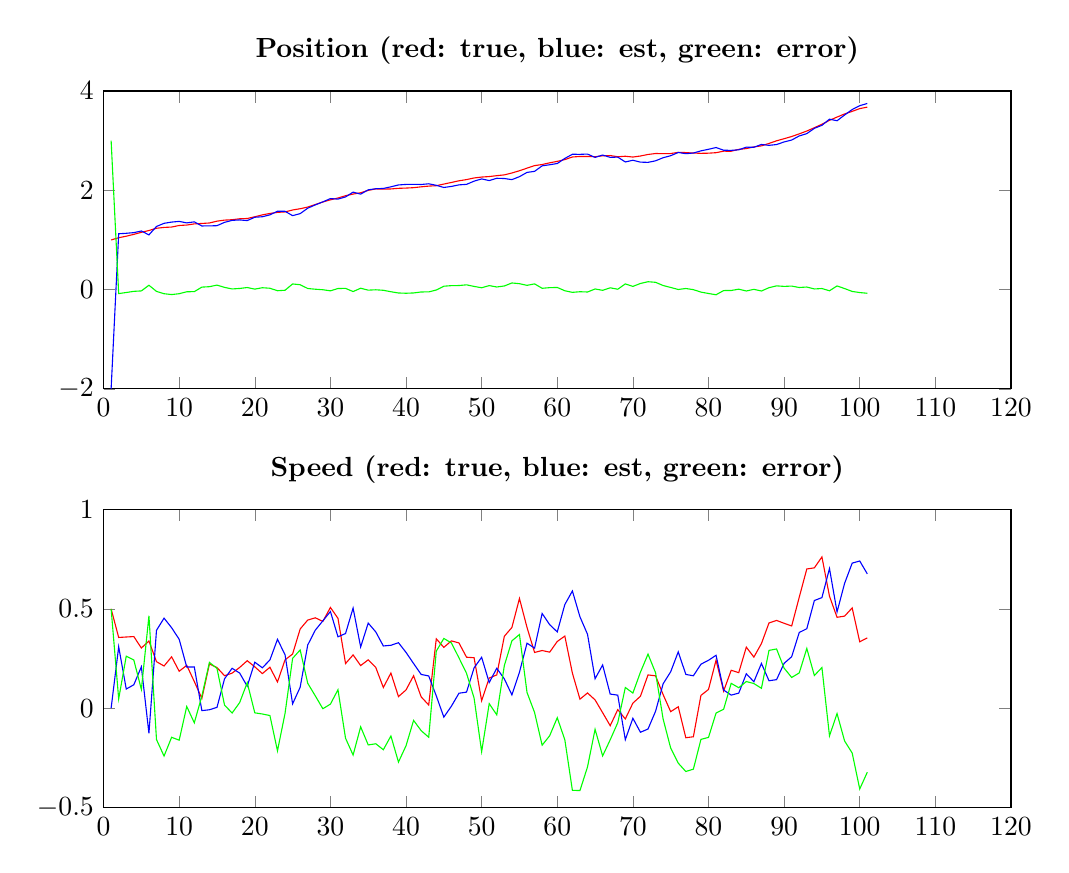
\begin{tikzpicture}

\begin{axis}[%
width=4.537in,
height=1.49in,
at={(0.761in,2.579in)},
scale only axis,
xmin=0,
xmax=120,
ymin=-2,
ymax=4,
axis background/.style={fill=white},
title style={font=\bfseries},
title={Position (red: true, blue: est, green: error)}
]
\addplot [color=red,solid,forget plot]
  table[row sep=crcr]{%
1	1\\
2	1.04434533272067\\
3	1.07549187610811\\
4	1.11216310550925\\
5	1.15371423954892\\
6	1.19008057998081\\
7	1.23538127592109\\
8	1.25219064180831\\
9	1.25983714964054\\
10	1.29108223589496\\
11	1.29988126345006\\
12	1.32335665283235\\
13	1.33186184233494\\
14	1.34147329667009\\
15	1.37815254061016\\
16	1.39942255452151\\
17	1.40719074502277\\
18	1.42611820019896\\
19	1.43184898196009\\
20	1.46688635865523\\
21	1.504950058184\\
22	1.5334947012432\\
23	1.55551343225254\\
24	1.56412088366082\\
25	1.60298756781952\\
26	1.6284403816137\\
27	1.66181241397372\\
28	1.71359847731262\\
29	1.76428142425421\\
30	1.80785028395092\\
31	1.84428773183073\\
32	1.89049197361164\\
33	1.92353984356575\\
34	1.95022299526192\\
35	1.99802968826035\\
36	2.02774105894173\\
37	2.02298148657876\\
38	2.02679223555182\\
39	2.03942902189953\\
40	2.04447723213062\\
41	2.05247597538524\\
42	2.06929824942615\\
43	2.08417513440982\\
44	2.09214557367989\\
45	2.12503242189789\\
46	2.15749679254932\\
47	2.19092883249404\\
48	2.21525065206297\\
49	2.24790458011253\\
50	2.26630003961527\\
51	2.27630384942826\\
52	2.29445110015679\\
53	2.31010858327454\\
54	2.34833256492697\\
55	2.39334858242299\\
56	2.44564408960361\\
57	2.49665575247235\\
58	2.51872349598708\\
59	2.55337661815382\\
60	2.58219560215773\\
61	2.6180942855088\\
62	2.66995552108672\\
63	2.68112827785137\\
64	2.68089839913975\\
65	2.67504508843955\\
66	2.69505345391533\\
67	2.69947470725191\\
68	2.67536325809254\\
69	2.68526654841314\\
70	2.66901047787169\\
71	2.69026989287448\\
72	2.72111430276888\\
73	2.7400714694544\\
74	2.738236970682\\
75	2.73951072834565\\
76	2.76382983571766\\
77	2.75913382374704\\
78	2.7497003855875\\
79	2.7439350654649\\
80	2.74702393127674\\
81	2.7571760906838\\
82	2.787350106959\\
83	2.78587920508525\\
84	2.82398508798126\\
85	2.8396351075773\\
86	2.87223111575936\\
87	2.89432839928876\\
88	2.94331850677609\\
89	2.99630117306705\\
90	3.03847947687699\\
91	3.08264008505478\\
92	3.13635348418202\\
93	3.19291095989198\\
94	3.25997806580483\\
95	3.32960785682653\\
96	3.40797870078894\\
97	3.4744046701411\\
98	3.53673142376042\\
99	3.58900981910119\\
100	3.6442554501847\\
101	3.67428798019773\\
};
\addplot [color=blue,solid,forget plot]
  table[row sep=crcr]{%
1	-2\\
2	1.12434885729259\\
3	1.1339862509674\\
4	1.14720367354413\\
5	1.18001770055632\\
6	1.10207944859836\\
7	1.27145573258207\\
8	1.33499439895226\\
9	1.35949271740574\\
10	1.37358868535333\\
11	1.34323594435174\\
12	1.3642277593336\\
13	1.281674247625\\
14	1.28250003607004\\
15	1.28735491240554\\
16	1.3546810769425\\
17	1.39401808439251\\
18	1.4029129280914\\
19	1.38986361732256\\
20	1.45706779661933\\
21	1.46714987143823\\
22	1.50583147810059\\
23	1.57820397898919\\
24	1.57696048676781\\
25	1.4891444990025\\
26	1.53013178221461\\
27	1.63932259913337\\
28	1.70578524667607\\
29	1.7668078852817\\
30	1.83259369439899\\
31	1.82226205872278\\
32	1.86576245431654\\
33	1.96282919551412\\
34	1.9223538926146\\
35	2.00899549680011\\
36	2.03117130711285\\
37	2.03675072177483\\
38	2.06968670242865\\
39	2.1073471916548\\
40	2.11773381882697\\
41	2.11981488118514\\
42	2.11685713079242\\
43	2.1303302339384\\
44	2.10001837864614\\
45	2.05664302741612\\
46	2.07763760722697\\
47	2.10890432795337\\
48	2.11905889489946\\
49	2.18376979185593\\
50	2.22884750553637\\
51	2.19536815900391\\
52	2.24174304701776\\
53	2.2369530387645\\
54	2.21444761188176\\
55	2.27407193757662\\
56	2.35994065051381\\
57	2.38117694905248\\
58	2.49230303847072\\
59	2.51381693035463\\
60	2.53895501744126\\
61	2.64128228556151\\
62	2.72514274399718\\
63	2.72380772558697\\
64	2.72907279755984\\
65	2.66233205134876\\
66	2.7093876753508\\
67	2.66316548101565\\
68	2.66774044801624\\
69	2.5704217856613\\
70	2.60444307180909\\
71	2.56676914054319\\
72	2.56220585822294\\
73	2.59322885367577\\
74	2.65584475156577\\
75	2.6962617067948\\
76	2.76112294044554\\
77	2.73674881522592\\
78	2.75052274607444\\
79	2.79389267277615\\
80	2.82528919876224\\
81	2.86098475650309\\
82	2.80654943636131\\
83	2.80375410427818\\
84	2.81497952746942\\
85	2.86770953098086\\
86	2.86646603285174\\
87	2.92252439344186\\
88	2.90466908918973\\
89	2.92103282860054\\
90	2.97347841210302\\
91	3.01158371449443\\
92	3.09404728223987\\
93	3.14095786556722\\
94	3.24681962262425\\
95	3.30786667014564\\
96	3.43141900592487\\
97	3.40040549893652\\
98	3.515695799806\\
99	3.62568585633203\\
100	3.70369159914067\\
101	3.74772549570158\\
};
\addplot [color=green,solid,forget plot]
  table[row sep=crcr]{%
1	3\\
2	-0.0800035245719242\\
3	-0.0584943748592932\\
4	-0.035040568034876\\
5	-0.0263034610073991\\
6	0.0880011313824534\\
7	-0.0360744566609779\\
8	-0.0828037571439544\\
9	-0.0996555677651982\\
10	-0.0825064494583692\\
11	-0.0433546809016734\\
12	-0.0408711065012517\\
13	0.0501875947099353\\
14	0.058973260600045\\
15	0.0907976282046248\\
16	0.044741477579012\\
17	0.0131726606302638\\
18	0.0232052721075535\\
19	0.0419853646375299\\
20	0.00981856203589992\\
21	0.0378001867457687\\
22	0.0276632231426091\\
23	-0.0226905467366487\\
24	-0.0128396031069928\\
25	0.113843068817022\\
26	0.0983085993990951\\
27	0.0224898148403485\\
28	0.00781323063654593\\
29	-0.00252646102748444\\
30	-0.0247434104480662\\
31	0.022025673107948\\
32	0.0247295192950994\\
33	-0.0392893519483695\\
34	0.0278691026473179\\
35	-0.0109658085397664\\
36	-0.00343024817112569\\
37	-0.0137692351960759\\
38	-0.0428944668768296\\
39	-0.0679181697552695\\
40	-0.0732565866963544\\
41	-0.0673389057999052\\
42	-0.0475588813662733\\
43	-0.0461550995285771\\
44	-0.0078728049662482\\
45	0.0683893944817626\\
46	0.0798591853223543\\
47	0.0820245045406733\\
48	0.0961917571635085\\
49	0.0641347882566032\\
50	0.0374525340788985\\
51	0.0809356904243552\\
52	0.0527080531390256\\
53	0.0731555445100422\\
54	0.133884953045215\\
55	0.11927664484637\\
56	0.0857034390897997\\
57	0.115478803419874\\
58	0.0264204575163616\\
59	0.0395596877991946\\
60	0.0432405847164659\\
61	-0.0231880000527114\\
62	-0.0551872229104573\\
63	-0.0426794477355958\\
64	-0.0481743984200884\\
65	0.0127130370907889\\
66	-0.0143342214354649\\
67	0.0363092262362583\\
68	0.00762281007630428\\
69	0.114844762751839\\
70	0.064567406062602\\
71	0.123500752331287\\
72	0.158908444545939\\
73	0.14684261577863\\
74	0.0823922191162332\\
75	0.0432490215508508\\
76	0.00270689527212609\\
77	0.0223850085211192\\
78	-0.000822360486939733\\
79	-0.0499576073112489\\
80	-0.0782652674854996\\
81	-0.103808665819292\\
82	-0.0191993294023098\\
83	-0.017874899192929\\
84	0.00900556051184243\\
85	-0.0280744234035577\\
86	0.00576508290761568\\
87	-0.0281959941531\\
88	0.0386494175863628\\
89	0.0752683444665099\\
90	0.0650010647739681\\
91	0.071056370560354\\
92	0.0423062019421563\\
93	0.0519530943247624\\
94	0.0131584431805796\\
95	0.0217411866808828\\
96	-0.0234403051359235\\
97	0.0739991712045791\\
98	0.0210356239544121\\
99	-0.0366760372308375\\
100	-0.05943614895597\\
101	-0.0734375155038505\\
};
\end{axis}

\begin{axis}[%
width=4.537in,
height=1.49in,
at={(0.761in,0.486in)},
scale only axis,
xmin=0,
xmax=120,
ymin=-0.5,
ymax=1,
axis background/.style={fill=white},
title style={font=\bfseries},
title={Speed (red: true, blue: est, green: error)}
]
\addplot [color=red,solid,forget plot]
  table[row sep=crcr]{%
1	0.5\\
2	0.356078056127843\\
3	0.358373809927211\\
4	0.360639692048267\\
5	0.302990516277225\\
6	0.338265577026095\\
7	0.234235233427978\\
8	0.212279356034809\\
9	0.25865685293472\\
10	0.185944785953524\\
11	0.215825263952482\\
12	0.134247328413475\\
13	0.0490593929002765\\
14	0.222905920748819\\
15	0.204436379389451\\
16	0.163609865201754\\
17	0.176550048106773\\
18	0.205203716916792\\
19	0.239011321488334\\
20	0.208210696449431\\
21	0.174275285024251\\
22	0.205965153579468\\
23	0.132063575685849\\
24	0.243074540380761\\
25	0.272787548509504\\
26	0.398784269389642\\
27	0.443667944054681\\
28	0.454996387734178\\
29	0.43698172490016\\
30	0.507128689505246\\
31	0.45243562644742\\
32	0.224663239282967\\
33	0.268292734083487\\
34	0.214513590332201\\
35	0.243590978553596\\
36	0.204856585768977\\
37	0.104228200798396\\
38	0.176984933299793\\
39	0.0585203745534094\\
40	0.0919366158868721\\
41	0.163557096431779\\
42	0.0570824442225027\\
43	0.0162066527782712\\
44	0.349265152722785\\
45	0.306273920458137\\
46	0.33881570401215\\
47	0.328577682578933\\
48	0.256648088588433\\
49	0.254060332504366\\
50	0.037426480222595\\
51	0.151784004442456\\
52	0.167635395448688\\
53	0.362100756593695\\
54	0.406279517738149\\
55	0.552082275821435\\
56	0.406461204015849\\
57	0.280719435307012\\
58	0.290325548331905\\
59	0.282099929369003\\
60	0.335986616138455\\
61	0.362999289558352\\
62	0.176675979728082\\
63	0.0454365596304139\\
64	0.0766785904238533\\
65	0.0418520532700866\\
66	-0.0225163829636803\\
67	-0.0879577033624556\\
68	-0.00725673188822407\\
69	-0.0540476048325951\\
70	0.0255239136630347\\
71	0.0601763948107619\\
72	0.167471743324591\\
73	0.163020088853704\\
74	0.0683283009182438\\
75	-0.0173854537076046\\
76	0.00717805505314287\\
77	-0.148563081119253\\
78	-0.143745692691517\\
79	0.0643686457338242\\
80	0.094481797110571\\
81	0.241823695716265\\
82	0.0861850040168673\\
83	0.190947198035838\\
84	0.178909349591918\\
85	0.307301405187384\\
86	0.257275333701059\\
87	0.325397994233586\\
88	0.429222716377165\\
89	0.441867863335602\\
90	0.427434048709204\\
91	0.413883680419612\\
92	0.558590689740538\\
93	0.700807695488493\\
94	0.706485231096073\\
95	0.761407846362104\\
96	0.563604085080593\\
97	0.457584038386655\\
98	0.463491565936621\\
99	0.504856574670535\\
100	0.334359286610901\\
101	0.35375191386555\\
};
\addplot [color=blue,solid,forget plot]
  table[row sep=crcr]{%
1	0\\
2	0.309341440391203\\
3	0.0965930822563975\\
4	0.117951428015327\\
5	0.208512561502614\\
6	-0.126868068322554\\
7	0.392027098083623\\
8	0.45324480423967\\
9	0.405039709997162\\
10	0.346875732063243\\
11	0.207150431630629\\
12	0.20773970899845\\
13	-0.012180120590336\\
14	-0.00781639329832481\\
15	0.00426287956667769\\
16	0.148056146916813\\
17	0.200882791768737\\
18	0.176755222423814\\
19	0.11050445124487\\
20	0.231587730762376\\
21	0.203394371577271\\
22	0.242933935970111\\
23	0.346563176364751\\
24	0.269191616454664\\
25	0.0219250234451926\\
26	0.10553027770555\\
27	0.318100109698366\\
28	0.392778636130537\\
29	0.439640164709449\\
30	0.486667877280606\\
31	0.359521154647631\\
32	0.375788381987388\\
33	0.503990300525852\\
34	0.308147694366762\\
35	0.428459682410649\\
36	0.383913590620876\\
37	0.313200845136942\\
38	0.316683248852123\\
39	0.329596909046207\\
40	0.280949901670066\\
41	0.224887519727396\\
42	0.170047991254955\\
43	0.162436864959951\\
44	0.0621054342546797\\
45	-0.0447566832566857\\
46	0.0101340205723036\\
47	0.0753326770032583\\
48	0.0809818155618705\\
49	0.202987372154971\\
50	0.256388322690174\\
51	0.128983264391156\\
52	0.201128302764602\\
53	0.147460418233537\\
54	0.0671801112879406\\
55	0.181198036489787\\
56	0.327203104788964\\
57	0.302454013396847\\
58	0.476759260687326\\
59	0.42037769487014\\
60	0.383957340519257\\
61	0.521735617637532\\
62	0.590023765173944\\
63	0.459991185163294\\
64	0.372205605877454\\
65	0.148159523666868\\
66	0.217638951581632\\
67	0.0711227383402797\\
68	0.0656546110831015\\
69	-0.158225134011331\\
70	-0.0508072075223234\\
71	-0.121048543910836\\
72	-0.104795769410349\\
73	-0.015353946939867\\
74	0.122897929789511\\
75	0.183514525519912\\
76	0.283747338674163\\
77	0.170068744364182\\
78	0.163101456560856\\
79	0.221417748606665\\
80	0.241362579961054\\
81	0.266273923427692\\
82	0.0915763969656712\\
83	0.0658166544184347\\
84	0.0758243751995788\\
85	0.17312149076299\\
86	0.13313238147547\\
87	0.225252012439647\\
88	0.13822834630217\\
89	0.143704227463078\\
90	0.225759665775916\\
91	0.259226798457769\\
92	0.381077560137124\\
93	0.400048454527795\\
94	0.541976095548723\\
95	0.556737258033068\\
96	0.703021843128005\\
97	0.484677303208095\\
98	0.628686027181049\\
99	0.730237050718612\\
100	0.740973795674217\\
101	0.676184252404593\\
};
\addplot [color=green,solid,forget plot]
  table[row sep=crcr]{%
1	0.5\\
2	0.0467366157366403\\
3	0.261780727670813\\
4	0.242688264032941\\
5	0.0944779547746106\\
6	0.465133645348649\\
7	-0.157791864655645\\
8	-0.240965448204861\\
9	-0.146382857062442\\
10	-0.160930946109719\\
11	0.0086748323218534\\
12	-0.0734923805849743\\
13	0.0612395134906125\\
14	0.230722314047144\\
15	0.200173499822774\\
16	0.0155537182849407\\
17	-0.0243327436619643\\
18	0.0284484944929778\\
19	0.128506870243464\\
20	-0.0233770343129456\\
21	-0.0291190865530203\\
22	-0.0369687823906431\\
23	-0.214499600678903\\
24	-0.0261170760739035\\
25	0.250862525064312\\
26	0.293253991684092\\
27	0.125567834356314\\
28	0.0622177516036407\\
29	-0.00265843980928898\\
30	0.0204608122246397\\
31	0.0929144717997895\\
32	-0.151125142704421\\
33	-0.235697566442365\\
34	-0.0936341040345611\\
35	-0.184868703857053\\
36	-0.1790570048519\\
37	-0.208972644338546\\
38	-0.13969831555233\\
39	-0.271076534492798\\
40	-0.189013285783194\\
41	-0.061330423295617\\
42	-0.112965547032453\\
43	-0.14623021218168\\
44	0.287159718468105\\
45	0.351030603714823\\
46	0.328681683439846\\
47	0.253245005575675\\
48	0.175666273026562\\
49	0.051072960349395\\
50	-0.218961842467579\\
51	0.0228007400512992\\
52	-0.0334929073159144\\
53	0.214640338360158\\
54	0.339099406450208\\
55	0.370884239331648\\
56	0.0792580992268854\\
57	-0.0217345780898352\\
58	-0.186433712355421\\
59	-0.138277765501136\\
60	-0.0479707243808016\\
61	-0.158736328079179\\
62	-0.413347785445862\\
63	-0.41455462553288\\
64	-0.295527015453601\\
65	-0.106307470396781\\
66	-0.240155334545312\\
67	-0.159080441702735\\
68	-0.0729113429713256\\
69	0.104177529178736\\
70	0.0763311211853581\\
71	0.181224938721598\\
72	0.27226751273494\\
73	0.178374035793571\\
74	-0.0545696288712676\\
75	-0.200899979227517\\
76	-0.27656928362102\\
77	-0.318631825483436\\
78	-0.306847149252372\\
79	-0.157049102872841\\
80	-0.146880782850483\\
81	-0.0244502277114262\\
82	-0.00539139294880386\\
83	0.125130543617403\\
84	0.103084974392339\\
85	0.134179914424394\\
86	0.124142952225589\\
87	0.100145981793938\\
88	0.290994370074995\\
89	0.298163635872524\\
90	0.201674382933287\\
91	0.154656881961843\\
92	0.177513129603414\\
93	0.300759240960699\\
94	0.16450913554735\\
95	0.204670588329036\\
96	-0.139417758047411\\
97	-0.0270932648214403\\
98	-0.165194461244428\\
99	-0.225380476048077\\
100	-0.406614509063316\\
101	-0.322432338539043\\
};
\end{axis}
\end{tikzpicture}%}
	\scalebox{0.5}{% This file was created by matlab2tikz.
%
%The latest updates can be retrieved from
%  http://www.mathworks.com/matlabcentral/fileexchange/22022-matlab2tikz-matlab2tikz
%where you can also make suggestions and rate matlab2tikz.
%
\definecolor{mycolor1}{rgb}{0.00000,0.44700,0.74100}%
%
\begin{tikzpicture}

\begin{axis}[%
width=4.521in,
height=1.474in,
at={(0.758in,2.554in)},
scale only axis,
xmin=0,
xmax=120,
ymin=0,
ymax=40,
axis background/.style={fill=white},
title style={font=\bfseries},
title={sqrt(P(1,1))}
]
\addplot [color=mycolor1,solid,forget plot]
  table[row sep=crcr]{%
1	31.6227766016838\\
2	0.0999995049539418\\
3	0.0999495911254347\\
4	0.0913186214638919\\
5	0.0838202432101647\\
6	0.0778367061085318\\
7	0.0731211925255747\\
8	0.0694423414240979\\
9	0.0666274565579433\\
10	0.0645399313436063\\
11	0.0630573615649224\\
12	0.0620604991411863\\
13	0.0614329284305988\\
14	0.0610674128439667\\
15	0.0608734615014402\\
16	0.0607819243647111\\
17	0.060745177693471\\
18	0.0607338331730901\\
19	0.0607318731604881\\
20	0.0607318710010368\\
21	0.0607312120902643\\
22	0.06072955106208\\
23	0.0607273383127599\\
24	0.0607251039042249\\
25	0.0607231977574287\\
26	0.0607217604246534\\
27	0.0607207824803978\\
28	0.0607201775304184\\
29	0.0607198379855147\\
30	0.0607196672092807\\
31	0.0607195924410309\\
32	0.0607195657264159\\
33	0.0607195591621504\\
34	0.0607195586538151\\
35	0.0607195583926261\\
36	0.0607195568471002\\
37	0.0607195542658778\\
38	0.0607195513472451\\
39	0.0607195486677513\\
40	0.0607195465311107\\
41	0.0607195450059272\\
42	0.0607195440184636\\
43	0.0607195434371509\\
44	0.0607195431281786\\
45	0.0607195429828141\\
46	0.0607195429248512\\
47	0.0607195429071839\\
48	0.0607195429042377\\
49	0.0607195429042376\\
50	0.0607195429030971\\
51	0.0607195429003293\\
52	0.0607195428966906\\
53	0.0607195428930426\\
54	0.0607195428899459\\
55	0.06071954288762\\
56	0.0607195428860431\\
57	0.060719542885071\\
58	0.0607195428845274\\
59	0.0607195428842552\\
60	0.0607195428841368\\
61	0.0607195428840949\\
62	0.0607195428840848\\
63	0.0607195428840841\\
64	0.0607195428840836\\
65	0.060719542884081\\
66	0.0607195428840767\\
67	0.0607195428840719\\
68	0.0607195428840676\\
69	0.0607195428840641\\
70	0.0607195428840616\\
71	0.06071954288406\\
72	0.0607195428840591\\
73	0.0607195428840586\\
74	0.0607195428840584\\
75	0.0607195428840583\\
76	0.0607195428840583\\
77	0.0607195428840583\\
78	0.0607195428840583\\
79	0.0607195428840583\\
80	0.0607195428840582\\
81	0.0607195428840582\\
82	0.0607195428840582\\
83	0.0607195428840582\\
84	0.0607195428840582\\
85	0.0607195428840582\\
86	0.0607195428840582\\
87	0.0607195428840582\\
88	0.0607195428840582\\
89	0.0607195428840582\\
90	0.0607195428840582\\
91	0.0607195428840582\\
92	0.0607195428840582\\
93	0.0607195428840582\\
94	0.0607195428840582\\
95	0.0607195428840582\\
96	0.0607195428840582\\
97	0.0607195428840582\\
98	0.0607195428840582\\
99	0.0607195428840582\\
100	0.0607195428840582\\
101	0.0607195428840582\\
};
\end{axis}

\begin{axis}[%
width=4.521in,
height=1.474in,
at={(0.758in,0.481in)},
scale only axis,
xmin=0,
xmax=120,
ymin=0,
ymax=40,
axis background/.style={fill=white},
title style={font=\bfseries},
title={sqrt(P(2,2))}
]
\addplot [color=mycolor1,solid,forget plot]
  table[row sep=crcr]{%
1	31.6227766016838\\
2	31.4659992517304\\
3	1.41981611922013\\
4	0.71918944041432\\
5	0.468114627120191\\
6	0.348995031784132\\
7	0.286171885234792\\
8	0.251942641004436\\
9	0.233427963964501\\
10	0.223747189720522\\
11	0.218973930336321\\
12	0.216824440134651\\
13	0.215985311658742\\
14	0.21573028878933\\
15	0.215686679479738\\
16	0.21568663933193\\
17	0.21567180012282\\
18	0.215634543738394\\
19	0.215584974268474\\
20	0.215534955863945\\
21	0.215492312335102\\
22	0.215460176428316\\
23	0.21543832463103\\
24	0.215424815281197\\
25	0.215417237420356\\
26	0.215413428691622\\
27	0.215411762629944\\
28	0.215411168149983\\
29	0.215411022489057\\
30	0.215411011354526\\
31	0.215411005395428\\
32	0.215410970647125\\
33	0.215410912784483\\
34	0.215410847447126\\
35	0.21541078751377\\
36	0.215410739752388\\
37	0.215410705676976\\
38	0.2154106836259\\
39	0.21541067065102\\
40	0.215410663758623\\
41	0.215410660518195\\
42	0.21541065922743\\
43	0.215410658834733\\
44	0.215410658769589\\
45	0.215410658769589\\
46	0.215410658743859\\
47	0.215410658681748\\
48	0.215410658600244\\
49	0.215410658518617\\
50	0.215410658449376\\
51	0.2154106583974\\
52	0.215410658362177\\
53	0.215410658340475\\
54	0.215410658328346\\
55	0.215410658322276\\
56	0.215410658319637\\
57	0.215410658318704\\
58	0.21541065831848\\
59	0.215410658318465\\
60	0.215410658318454\\
61	0.215410658318395\\
62	0.215410658318299\\
63	0.215410658318192\\
64	0.215410658318095\\
65	0.215410658318017\\
66	0.215410658317962\\
67	0.215410658317927\\
68	0.215410658317906\\
69	0.215410658317895\\
70	0.21541065831789\\
71	0.215410658317888\\
72	0.215410658317887\\
73	0.215410658317887\\
74	0.215410658317887\\
75	0.215410658317887\\
76	0.215410658317887\\
77	0.215410658317887\\
78	0.215410658317886\\
79	0.215410658317886\\
80	0.215410658317886\\
81	0.215410658317886\\
82	0.215410658317886\\
83	0.215410658317886\\
84	0.215410658317886\\
85	0.215410658317886\\
86	0.215410658317886\\
87	0.215410658317886\\
88	0.215410658317886\\
89	0.215410658317886\\
90	0.215410658317886\\
91	0.215410658317886\\
92	0.215410658317886\\
93	0.215410658317886\\
94	0.215410658317886\\
95	0.215410658317886\\
96	0.215410658317886\\
97	0.215410658317886\\
98	0.215410658317886\\
99	0.215410658317886\\
100	0.215410658317886\\
101	0.215410658317886\\
};
\end{axis}
\end{tikzpicture}%}
	\scalebox{0.5}{% This file was created by matlab2tikz.
%
%The latest updates can be retrieved from
%  http://www.mathworks.com/matlabcentral/fileexchange/22022-matlab2tikz-matlab2tikz
%where you can also make suggestions and rate matlab2tikz.
%
\definecolor{mycolor1}{rgb}{0.00000,0.44700,0.74100}%
%
\begin{tikzpicture}

\begin{axis}[%
width=4.521in,
height=1.474in,
at={(0.758in,2.554in)},
scale only axis,
xmin=0,
xmax=100,
ymin=0.2,
ymax=1,
axis background/.style={fill=white},
title style={font=\bfseries},
title={K(1)}
]
\addplot [color=mycolor1,solid,forget plot]
  table[row sep=crcr]{%
1	0.99999009910891\\
2	0.99899207661427\\
3	0.833909062606559\\
4	0.702583317181116\\
5	0.605855281782595\\
6	0.534670879636216\\
7	0.482223878246099\\
8	0.443921796738062\\
9	0.416540273783741\\
10	0.397623084752935\\
11	0.385150555365319\\
12	0.377400469555908\\
13	0.372922891145547\\
14	0.370557831516732\\
15	0.369444232947746\\
16	0.368997661301136\\
17	0.368859849189674\\
18	0.368836041758161\\
19	0.368836015528657\\
20	0.368828012195266\\
21	0.368807837220179\\
22	0.36878096185524\\
23	0.368753824417891\\
24	0.368730674588779\\
25	0.3687132189069\\
26	0.368701342503178\\
27	0.368693995932552\\
28	0.368689872498715\\
29	0.36868779860058\\
30	0.36868689062049\\
31	0.368686566200454\\
32	0.368686486484588\\
33	0.368686480311409\\
34	0.368686477139553\\
35	0.368686458370823\\
36	0.368686427024687\\
37	0.368686391581073\\
38	0.368686359041542\\
39	0.368686333094372\\
40	0.368686314572682\\
41	0.368686302581013\\
42	0.368686295521606\\
43	0.368686291769474\\
44	0.368686290004181\\
45	0.368686289300285\\
46	0.368686289085735\\
47	0.368686289049956\\
48	0.368686289049955\\
49	0.368686289036105\\
50	0.368686289002493\\
51	0.368686288958304\\
52	0.368686288914003\\
53	0.368686288876397\\
54	0.368686288848153\\
55	0.368686288829003\\
56	0.368686288817198\\
57	0.368686288810596\\
58	0.368686288807291\\
59	0.368686288805853\\
60	0.368686288805343\\
61	0.368686288805221\\
62	0.368686288805212\\
63	0.368686288805206\\
64	0.368686288805175\\
65	0.368686288805123\\
66	0.368686288805065\\
67	0.368686288805012\\
68	0.36868628880497\\
69	0.36868628880494\\
70	0.36868628880492\\
71	0.368686288804909\\
72	0.368686288804903\\
73	0.3686862888049\\
74	0.368686288804899\\
75	0.368686288804899\\
76	0.368686288804899\\
77	0.368686288804899\\
78	0.368686288804899\\
79	0.368686288804899\\
80	0.368686288804899\\
81	0.368686288804899\\
82	0.368686288804899\\
83	0.368686288804899\\
84	0.368686288804899\\
85	0.368686288804899\\
86	0.368686288804899\\
87	0.368686288804899\\
88	0.368686288804899\\
89	0.368686288804899\\
90	0.368686288804899\\
91	0.368686288804899\\
92	0.368686288804899\\
93	0.368686288804899\\
94	0.368686288804899\\
95	0.368686288804899\\
96	0.368686288804899\\
97	0.368686288804899\\
98	0.368686288804899\\
99	0.368686288804899\\
100	0.368686288804899\\
};
\end{axis}

\begin{axis}[%
width=4.521in,
height=1.474in,
at={(0.758in,0.481in)},
scale only axis,
xmin=0,
xmax=100,
ymin=0,
ymax=10,
axis background/.style={fill=white},
title style={font=\bfseries},
title={K(2)}
]
\addplot [color=mycolor1,solid,forget plot]
  table[row sep=crcr]{%
1	0.09900891090099\\
2	9.97964104634358\\
3	5.00571829155446\\
4	3.02712270239892\\
5	2.0568188857117\\
6	1.52385710809347\\
7	1.21304620202199\\
8	1.02751971670938\\
9	0.917435492760526\\
10	0.854208741957208\\
11	0.820027510252535\\
12	0.80325045047291\\
13	0.796229277107124\\
14	0.794119882729789\\
15	0.794076104093574\\
16	0.794610750265193\\
17	0.795081332035254\\
18	0.795306916595436\\
19	0.795314417156249\\
20	0.795193130613918\\
21	0.795025976870823\\
22	0.794866899613724\\
23	0.794741218156603\\
24	0.794654280853559\\
25	0.794600761403418\\
26	0.794571564389591\\
27	0.794557847358518\\
28	0.79455276050259\\
29	0.794551763096631\\
30	0.794552245895254\\
31	0.794552942790319\\
32	0.794553388567956\\
33	0.794553520385851\\
34	0.794553429889383\\
35	0.794553233370675\\
36	0.794553018854032\\
37	0.794552835355584\\
38	0.794552700488543\\
39	0.794552612711959\\
40	0.794552561862072\\
41	0.794552536038771\\
42	0.79455252511026\\
43	0.794552521865193\\
44	0.794552521861101\\
45	0.794552522744419\\
46	0.794552523502116\\
47	0.794552523856558\\
48	0.794552523858646\\
49	0.794552523655385\\
50	0.794552523381042\\
51	0.794552523122092\\
52	0.794552522918571\\
53	0.794552522778388\\
54	0.794552522692447\\
55	0.794552522645784\\
56	0.794552522624005\\
57	0.794552522616027\\
58	0.794552522614541\\
59	0.794552522615371\\
60	0.794552522616506\\
61	0.794552522617217\\
62	0.794552522617416\\
63	0.794552522617258\\
64	0.794552522616933\\
65	0.794552522616582\\
66	0.794552522616284\\
67	0.794552522616066\\
68	0.794552522615925\\
69	0.794552522615843\\
70	0.794552522615802\\
71	0.794552522615785\\
72	0.79455252261578\\
73	0.79455252261578\\
74	0.794552522615782\\
75	0.794552522615783\\
76	0.794552522615783\\
77	0.794552522615783\\
78	0.794552522615783\\
79	0.794552522615783\\
80	0.794552522615782\\
81	0.794552522615782\\
82	0.794552522615782\\
83	0.794552522615781\\
84	0.794552522615781\\
85	0.794552522615781\\
86	0.794552522615781\\
87	0.794552522615781\\
88	0.794552522615781\\
89	0.794552522615781\\
90	0.794552522615781\\
91	0.794552522615781\\
92	0.794552522615781\\
93	0.794552522615781\\
94	0.794552522615781\\
95	0.794552522615781\\
96	0.794552522615781\\
97	0.794552522615781\\
98	0.794552522615781\\
99	0.794552522615781\\
100	0.794552522615781\\
};
\end{axis}
\end{tikzpicture}%}

	\caption{$P_0' = P_0 \times 1000$}
	\label{fig:q4:P1000}
\end{figure}

\begin{figure}[H]
	\scalebox{0.5}{% This file was created by matlab2tikz.
%
%The latest updates can be retrieved from
%  http://www.mathworks.com/matlabcentral/fileexchange/22022-matlab2tikz-matlab2tikz
%where you can also make suggestions and rate matlab2tikz.
%
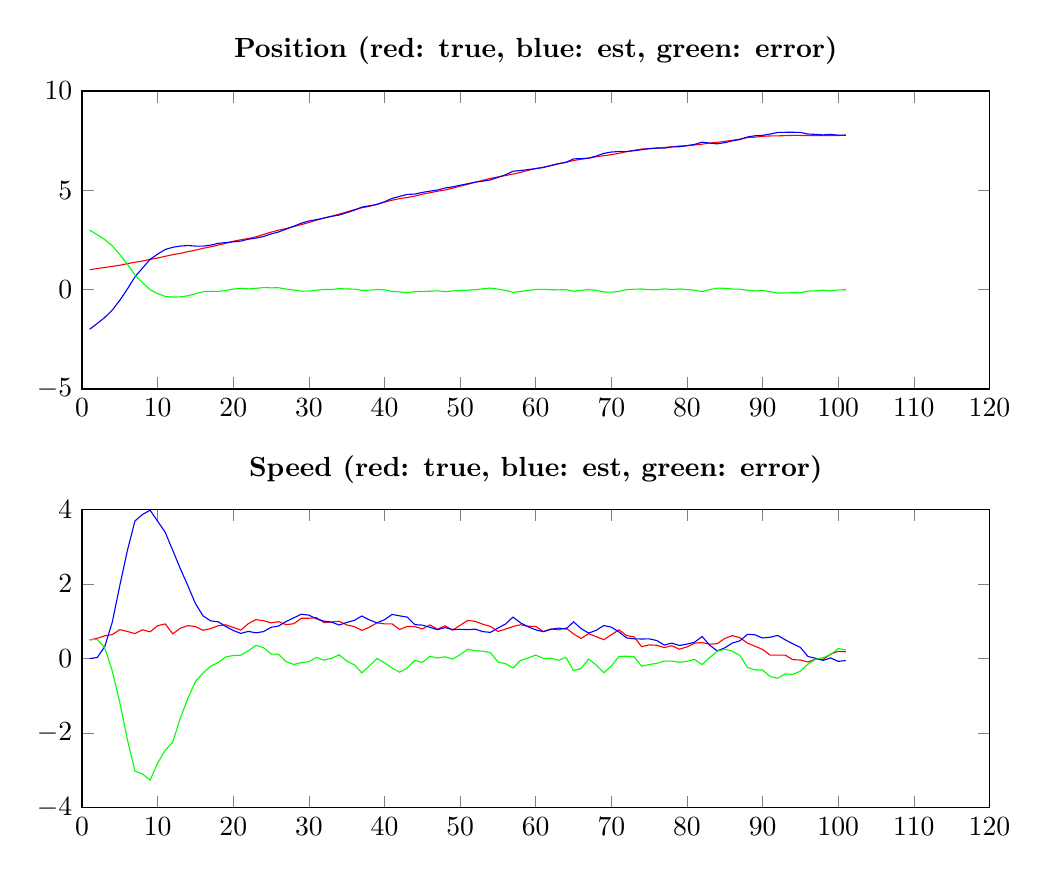
\begin{tikzpicture}

\begin{axis}[%
width=4.537in,
height=1.49in,
at={(0.761in,2.579in)},
scale only axis,
xmin=0,
xmax=120,
ymin=-5,
ymax=10,
axis background/.style={fill=white},
title style={font=\bfseries},
title={Position (red: true, blue: est, green: error)}
]
\addplot [color=red,solid,forget plot]
  table[row sep=crcr]{%
1	1\\
2	1.06000373502673\\
3	1.11492620942438\\
4	1.16909274937911\\
5	1.22658880515531\\
6	1.30870643588775\\
7	1.37660493713512\\
8	1.43864204832079\\
9	1.51970344501093\\
10	1.59223516378117\\
11	1.67722787150996\\
12	1.75806887714625\\
13	1.82697786742872\\
14	1.90954777170756\\
15	1.98776430292313\\
16	2.07887704354838\\
17	2.15515620366155\\
18	2.24094296229144\\
19	2.32688328889819\\
20	2.43265322988398\\
21	2.50986473815892\\
22	2.57362595376839\\
23	2.65821232254184\\
24	2.77804981055487\\
25	2.8928316380089\\
26	2.99610501849743\\
27	3.07394767387362\\
28	3.17579637663887\\
29	3.27256539212213\\
30	3.37479564475028\\
31	3.4958939079647\\
32	3.60533640051731\\
33	3.69315284154591\\
34	3.80284431231624\\
35	3.90743607386826\\
36	4.0221356961676\\
37	4.11946442872483\\
38	4.191175840858\\
39	4.29252958030054\\
40	4.4068002868159\\
41	4.50176327345838\\
42	4.5795125892307\\
43	4.6358379817582\\
44	4.70715154262758\\
45	4.80233065900021\\
46	4.87420725363944\\
47	4.95264199812621\\
48	5.01164416925442\\
49	5.10619778338663\\
50	5.20504024106525\\
51	5.30282357746104\\
52	5.40423475949451\\
53	5.50169055729297\\
54	5.59990664813693\\
55	5.67267958984228\\
56	5.7417897056089\\
57	5.81806257874149\\
58	5.90090460197034\\
59	6.00274587376474\\
60	6.09604522631668\\
61	6.16082908697837\\
62	6.24108555723882\\
63	6.33072639770484\\
64	6.40747674937204\\
65	6.49966569603215\\
66	6.56320747373889\\
67	6.61671806637243\\
68	6.68784957770567\\
69	6.74101642365891\\
70	6.79451959104202\\
71	6.86041274974685\\
72	6.9431977853086\\
73	7.01263675934944\\
74	7.07472487124058\\
75	7.09588133331623\\
76	7.11723979087122\\
77	7.15816817063411\\
78	7.18684041305187\\
79	7.22788734040044\\
80	7.24626952282184\\
81	7.28102532407278\\
82	7.3207047871376\\
83	7.37815869010184\\
84	7.41278626328141\\
85	7.46570916237091\\
86	7.51587482393341\\
87	7.57619535944723\\
88	7.65084837989051\\
89	7.67397392813472\\
90	7.71818753126647\\
91	7.73450936304315\\
92	7.73876718808748\\
93	7.75156219190918\\
94	7.76308062850609\\
95	7.76021577938967\\
96	7.7583321426646\\
97	7.75552564359379\\
98	7.7549990887126\\
99	7.75055726123844\\
100	7.75882331824041\\
101	7.77104703723544\\
};
\addplot [color=blue,solid,forget plot]
  table[row sep=crcr]{%
1	-2\\
2	-1.70731587969064\\
3	-1.40399826210713\\
4	-1.03352101242981\\
5	-0.53333869879605\\
6	0.0323169525948696\\
7	0.643315817118301\\
8	1.08624862432425\\
9	1.52359530488548\\
10	1.78759595652377\\
11	2.01951305067145\\
12	2.13121459475606\\
13	2.19364275841789\\
14	2.21944311038423\\
15	2.19265022436842\\
16	2.18702164754628\\
17	2.23915533154875\\
18	2.32885195654734\\
19	2.37014556872494\\
20	2.40523687974986\\
21	2.4442181414853\\
22	2.53699010948109\\
23	2.59238236047757\\
24	2.67614539861398\\
25	2.80200284128633\\
26	2.90293166662982\\
27	3.0463978660322\\
28	3.19115064215221\\
29	3.34544834434319\\
30	3.45356742535019\\
31	3.52384112431921\\
32	3.60160425315481\\
33	3.68976250624217\\
34	3.75139834869304\\
35	3.87338786113634\\
36	3.99683390886958\\
37	4.15307359569962\\
38	4.21951916508751\\
39	4.28672539135219\\
40	4.42132826675077\\
41	4.59171252188937\\
42	4.69198686171735\\
43	4.79182694721708\\
44	4.80887701222917\\
45	4.89360223637581\\
46	4.95683540042045\\
47	5.01041357398997\\
48	5.11419779637174\\
49	5.17259299973116\\
50	5.25379232875487\\
51	5.32852773819824\\
52	5.41145584439936\\
53	5.46021912719697\\
54	5.52269873771293\\
55	5.64764406533814\\
56	5.77894438114222\\
57	5.95862118328848\\
58	5.99640591534874\\
59	6.0436747105849\\
60	6.09148605987861\\
61	6.14578572731494\\
62	6.24662524256782\\
63	6.3411663867919\\
64	6.41044345807197\\
65	6.58037823930843\\
66	6.59414450470358\\
67	6.6184452571105\\
68	6.72235541927968\\
69	6.85744459169924\\
70	6.92555623057388\\
71	6.95053874365542\\
72	6.94791878616163\\
73	6.99171136265597\\
74	7.04249143426628\\
75	7.09645814257549\\
76	7.12914894721444\\
77	7.12070706692517\\
78	7.18126233803714\\
79	7.1932210174845\\
80	7.24539997449156\\
81	7.30800483159644\\
82	7.42256013729405\\
83	7.37478070244702\\
84	7.33793275458579\\
85	7.39747781301647\\
86	7.48627695505854\\
87	7.55527996035593\\
88	7.68391926737255\\
89	7.74251862583442\\
90	7.76697587338932\\
91	7.83193893049915\\
92	7.91168371208343\\
93	7.91844634794414\\
94	7.91994163471158\\
95	7.91421925192805\\
96	7.83112349870818\\
97	7.81426055102446\\
98	7.78851376233294\\
99	7.81417080800152\\
100	7.77341747547753\\
101	7.77544739499413\\
};
\addplot [color=green,solid,forget plot]
  table[row sep=crcr]{%
1	3\\
2	2.76731961471737\\
3	2.51892447153151\\
4	2.20261376180892\\
5	1.75992750395136\\
6	1.27638948329288\\
7	0.733289120016816\\
8	0.352393423996547\\
9	-0.00389185987454299\\
10	-0.195360792742597\\
11	-0.342285179161488\\
12	-0.373145717609811\\
13	-0.366664890989165\\
14	-0.309895338676678\\
15	-0.204885921445287\\
16	-0.108144603997897\\
17	-0.0839991278872017\\
18	-0.0879089942559044\\
19	-0.0432622798267519\\
20	0.0274163501341134\\
21	0.065646596673623\\
22	0.0366358442873045\\
23	0.0658299620642704\\
24	0.101904411940892\\
25	0.0908287967225654\\
26	0.0931733518676077\\
27	0.0275498078414169\\
28	-0.0153542655133418\\
29	-0.0728829522210557\\
30	-0.0787717805999106\\
31	-0.0279472163545167\\
32	0.0037321473625016\\
33	0.00339033530373367\\
34	0.0514459636231961\\
35	0.034048212731919\\
36	0.0253017872980212\\
37	-0.033609166974788\\
38	-0.0283433242295095\\
39	0.00580418894834889\\
40	-0.0145279799348703\\
41	-0.089949248430985\\
42	-0.112474272486654\\
43	-0.155988965458887\\
44	-0.101725469601593\\
45	-0.0912715773756068\\
46	-0.0826281467810039\\
47	-0.0577715758637671\\
48	-0.102553627117313\\
49	-0.0663952163445298\\
50	-0.0487520876896239\\
51	-0.0257041607371926\\
52	-0.00722108490485596\\
53	0.0414714300959966\\
54	0.0772079104240015\\
55	0.0250355245041405\\
56	-0.037154675533321\\
57	-0.140558604546998\\
58	-0.0955013133783993\\
59	-0.0409288368201635\\
60	0.00455916643807264\\
61	0.0150433596634292\\
62	-0.0055396853290075\\
63	-0.010439989087061\\
64	-0.00296670869993232\\
65	-0.0807125432762836\\
66	-0.0309370309646839\\
67	-0.00172719073806959\\
68	-0.0345058415740143\\
69	-0.116428168040334\\
70	-0.131036639531856\\
71	-0.0901259939085612\\
72	-0.00472100085303229\\
73	0.020925396693471\\
74	0.0322334369742991\\
75	-0.000576809259258404\\
76	-0.0119091563432132\\
77	0.0374611037089467\\
78	0.00557807501473118\\
79	0.0346663229159363\\
80	0.000869548330281411\\
81	-0.0269795075236647\\
82	-0.101855350156451\\
83	0.00337798765481434\\
84	0.074853508695619\\
85	0.0682313493544457\\
86	0.0295978688748759\\
87	0.0209153990913045\\
88	-0.0330708874820393\\
89	-0.0685446976996928\\
90	-0.0487883421228466\\
91	-0.097429567455996\\
92	-0.172916523995951\\
93	-0.166884156034958\\
94	-0.156861006205495\\
95	-0.154003472538379\\
96	-0.0727913560435818\\
97	-0.0587349074306696\\
98	-0.0335146736203376\\
99	-0.0636135467630865\\
100	-0.0145941572371271\\
101	-0.0044003577586933\\
};
\end{axis}

\begin{axis}[%
width=4.537in,
height=1.49in,
at={(0.761in,0.486in)},
scale only axis,
xmin=0,
xmax=120,
ymin=-4,
ymax=4,
axis background/.style={fill=white},
title style={font=\bfseries},
title={Speed (red: true, blue: est, green: error)}
]
\addplot [color=red,solid,forget plot]
  table[row sep=crcr]{%
1	0.5\\
2	0.543710429413519\\
3	0.611097071992505\\
4	0.643129672065997\\
5	0.775710528791875\\
6	0.726829273395776\\
7	0.670675799825701\\
8	0.771714961422398\\
9	0.718492757073892\\
10	0.881678209525629\\
11	0.929203536231283\\
12	0.664198951727828\\
13	0.81651762189318\\
14	0.883564957296546\\
15	0.860572875812195\\
16	0.756937563349461\\
17	0.804777391337511\\
18	0.880195310639263\\
19	0.906730051701771\\
20	0.834732794919087\\
21	0.765306619171041\\
22	0.938240363171962\\
23	1.0449511312341\\
24	1.01578822639577\\
25	0.960017749585393\\
26	0.989055835663118\\
27	0.910845362941288\\
28	0.935408729883514\\
29	1.08063401942155\\
30	1.08265012528522\\
31	1.09741532686306\\
32	0.964117781582586\\
33	0.982348326915186\\
34	1.00199154461391\\
35	0.902470316768726\\
36	0.858706084147209\\
37	0.757196891140233\\
38	0.840466400803918\\
39	0.959786081528347\\
40	0.931842138263351\\
41	0.931354889297309\\
42	0.77961030182138\\
43	0.861775842096133\\
44	0.858523234908488\\
45	0.795196410686211\\
46	0.902936262512555\\
47	0.787826644567377\\
48	0.879401370185605\\
49	0.764653930725497\\
50	0.890421979398274\\
51	1.02476342985991\\
52	0.997785777499293\\
53	0.921374196245636\\
54	0.86486310362839\\
55	0.727506615376017\\
56	0.789411720633419\\
57	0.861956961674776\\
58	0.906717925997053\\
59	0.866695596508205\\
60	0.86452031918351\\
61	0.723733359090096\\
62	0.793626016300022\\
63	0.773688941982947\\
64	0.81861201459171\\
65	0.662443312538946\\
66	0.539232776589167\\
67	0.669412785774607\\
68	0.58683554477899\\
69	0.507084045386966\\
70	0.637904697179139\\
71	0.773244800013654\\
72	0.617867124543598\\
73	0.582456959995892\\
74	0.319551846814798\\
75	0.366784774258484\\
76	0.356850000589223\\
77	0.294280009538755\\
78	0.344409726191393\\
79	0.250734930965491\\
80	0.312460442306006\\
81	0.414210833732457\\
82	0.430371378818313\\
83	0.385517823224147\\
84	0.398940857878017\\
85	0.540873788287021\\
86	0.616014345607408\\
87	0.560381138353123\\
88	0.414878514347813\\
89	0.331185126607256\\
90	0.244836471997191\\
91	0.0907147762017073\\
92	0.0937727189512956\\
93	0.0911523782209862\\
94	-0.0294886297687225\\
95	-0.0383880189164426\\
96	-0.0931837318938206\\
97	-0.0144389623737808\\
98	-0.0234131582345259\\
99	0.119946013570775\\
100	0.19391830716789\\
101	0.181692310777782\\
};
\addplot [color=blue,solid,forget plot]
  table[row sep=crcr]{%
1	0\\
2	0.0263679387666088\\
3	0.317939895738993\\
4	0.978475467144923\\
5	1.96408756978372\\
6	2.90314740542683\\
7	3.69477729841767\\
8	3.86810864479613\\
9	3.98267119611108\\
10	3.68689242436813\\
11	3.39071772760053\\
12	2.90240251813975\\
13	2.4143856050778\\
14	1.95225250818583\\
15	1.47571604164234\\
16	1.14636052112475\\
17	1.0118239008126\\
18	0.987081302658988\\
19	0.863348343212807\\
20	0.752896718949812\\
21	0.674634954168135\\
22	0.729184581058804\\
23	0.691410715289161\\
24	0.722923766922221\\
25	0.838363094645235\\
26	0.875199001118896\\
27	0.995767544539215\\
28	1.09312523174345\\
29	1.19007178680509\\
30	1.1666070405975\\
31	1.06663904365636\\
32	1.00435529983375\\
33	0.97789665575637\\
34	0.899981864823132\\
35	0.968926100899628\\
36	1.02615118859072\\
37	1.14171703182598\\
38	1.03886285955578\\
39	0.959813988328498\\
40	1.04304678754077\\
41	1.18545429057523\\
42	1.14607843002705\\
43	1.11425256823897\\
44	0.910865438005639\\
45	0.897156214983533\\
46	0.840084107954563\\
47	0.774504175990113\\
48	0.831255923087091\\
49	0.777959683094803\\
50	0.785294235324585\\
51	0.777117789501828\\
52	0.78835944969495\\
53	0.723550124483629\\
54	0.702267734127176\\
55	0.820191200780316\\
56	0.926396664802672\\
57	1.11396961721153\\
58	0.955328559629921\\
59	0.851315114144212\\
60	0.770886766636471\\
61	0.721774376728657\\
62	0.783543763701055\\
63	0.818427722291057\\
64	0.791347492592647\\
65	0.987029829180087\\
66	0.80398346911807\\
67	0.683088045067945\\
68	0.759812212464812\\
69	0.887195229238924\\
70	0.84278336268921\\
71	0.714995464617838\\
72	0.555261184740425\\
73	0.529974333392054\\
74	0.525195716967358\\
75	0.528314428134333\\
76	0.484909518989217\\
77	0.36221408168011\\
78	0.414655772011984\\
79	0.351065720641002\\
80	0.387858264696451\\
81	0.43919044452565\\
82	0.591418019199837\\
83	0.360993018395468\\
84	0.20378505317517\\
85	0.288192541392606\\
86	0.417454661212334\\
87	0.476197140036038\\
88	0.650801740110718\\
89	0.63683499250012\\
90	0.552298848402819\\
91	0.573274720884788\\
92	0.621586064026638\\
93	0.502202703502075\\
94	0.397195927292435\\
95	0.29926433240357\\
96	0.0556912294964474\\
97	0.0073480747590871\\
98	-0.0497221762283554\\
99	0.0162866750716116\\
100	-0.0750503940323383\\
101	-0.0545016893670609\\
};
\addplot [color=green,solid,forget plot]
  table[row sep=crcr]{%
1	0.5\\
2	0.51734249064691\\
3	0.293157176253512\\
4	-0.335345795078926\\
5	-1.18837704099184\\
6	-2.17631813203105\\
7	-3.02410149859197\\
8	-3.09639368337373\\
9	-3.26417843903718\\
10	-2.8052142148425\\
11	-2.46151419136924\\
12	-2.23820356641192\\
13	-1.59786798318462\\
14	-1.06868755088929\\
15	-0.615143165830144\\
16	-0.389422957775284\\
17	-0.207046509475088\\
18	-0.106885992019725\\
19	0.0433817084889642\\
20	0.0818360759692748\\
21	0.0906716650029057\\
22	0.209055782113158\\
23	0.353540415944942\\
24	0.292864459473551\\
25	0.121654654940158\\
26	0.113856834544222\\
27	-0.0849221815979274\\
28	-0.157716501859934\\
29	-0.109437767383544\\
30	-0.0839569153122863\\
31	0.0307762832066978\\
32	-0.0402375182511608\\
33	0.0044516711588154\\
34	0.102009679790782\\
35	-0.066455784130902\\
36	-0.167445104443513\\
37	-0.384520140685748\\
38	-0.198396458751862\\
39	-2.79068001506344e-05\\
40	-0.111204649277423\\
41	-0.254099401277922\\
42	-0.366468128205672\\
43	-0.252476726142836\\
44	-0.052342203097151\\
45	-0.101959804297321\\
46	0.062852154557992\\
47	0.0133224685772646\\
48	0.0481454470985138\\
49	-0.0133057523693059\\
50	0.105127744073689\\
51	0.247645640358086\\
52	0.209426327804344\\
53	0.197824071762007\\
54	0.162595369501214\\
55	-0.0926845854042992\\
56	-0.136984944169253\\
57	-0.252012655536751\\
58	-0.0486106336328674\\
59	0.0153804823639937\\
60	0.093633552547039\\
61	0.00195898236143965\\
62	0.0100822525989666\\
63	-0.04473878030811\\
64	0.0272645219990632\\
65	-0.324586516641141\\
66	-0.264750692528903\\
67	-0.0136752592933379\\
68	-0.172976667685823\\
69	-0.380111183851958\\
70	-0.204878665510071\\
71	0.0582493353958156\\
72	0.0626059398031731\\
73	0.0524826266038381\\
74	-0.20564387015256\\
75	-0.16152965387585\\
76	-0.128059518399994\\
77	-0.0679340721413543\\
78	-0.0702460458205916\\
79	-0.10033078967551\\
80	-0.0753978223904453\\
81	-0.0249796107931923\\
82	-0.161046640381524\\
83	0.0245248048286786\\
84	0.195155804702847\\
85	0.252681246894415\\
86	0.198559684395074\\
87	0.0841839983170845\\
88	-0.235923225762905\\
89	-0.305649865892864\\
90	-0.307462376405629\\
91	-0.48255994468308\\
92	-0.527813345075343\\
93	-0.411050325281089\\
94	-0.426684557061158\\
95	-0.337652351320012\\
96	-0.148874961390268\\
97	-0.0217870371328679\\
98	0.0263090179938295\\
99	0.103659338499163\\
100	0.268968701200228\\
101	0.236194000144843\\
};
\end{axis}
\end{tikzpicture}%}
	\scalebox{0.5}{% This file was created by matlab2tikz.
%
%The latest updates can be retrieved from
%  http://www.mathworks.com/matlabcentral/fileexchange/22022-matlab2tikz-matlab2tikz
%where you can also make suggestions and rate matlab2tikz.
%
\definecolor{mycolor1}{rgb}{0.00000,0.44700,0.74100}%
%
\begin{tikzpicture}

\begin{axis}[%
width=4.521in,
height=1.474in,
at={(0.758in,2.554in)},
scale only axis,
xmin=0,
xmax=120,
ymin=0.03,
ymax=0.07,
axis background/.style={fill=white},
title style={font=\bfseries},
title={sqrt(P(1,1))}
]
\addplot [color=mycolor1,solid,forget plot]
  table[row sep=crcr]{%
1	0.0316227766016838\\
2	0.0316085417251571\\
3	0.0330601662689741\\
4	0.0372754982908906\\
5	0.0434830783581549\\
6	0.0497599875578998\\
7	0.0546411903282231\\
8	0.0577477952407754\\
9	0.0594256895141182\\
10	0.0602007737165512\\
11	0.0604967623576609\\
12	0.0605795514108495\\
13	0.0605900273840077\\
14	0.0605902649566987\\
15	0.0605998399340386\\
16	0.0606192766628066\\
17	0.0606431454353206\\
18	0.0606661578632279\\
19	0.0606851573836185\\
20	0.0606991058798251\\
21	0.0607083677717021\\
22	0.0607139591462845\\
23	0.060717014699293\\
24	0.0607185024229526\\
25	0.060719125217714\\
26	0.0607193317839906\\
27	0.0607193745178996\\
28	0.060719375429412\\
29	0.0607193810848102\\
30	0.0607194008642175\\
31	0.0607194298963512\\
32	0.0607194607192021\\
33	0.0607194878980301\\
34	0.0607195089208824\\
35	0.060719523543358\\
36	0.0607195327816481\\
37	0.0607195380836013\\
38	0.0607195408205009\\
39	0.0607195420605225\\
40	0.0607195425277375\\
41	0.0607195426555264\\
42	0.0607195426704802\\
43	0.0607195426712552\\
44	0.0607195426880105\\
45	0.0607195427206769\\
46	0.0607195427601224\\
47	0.0607195427977852\\
48	0.0607195428286791\\
49	0.0607195428512504\\
50	0.0607195428661779\\
51	0.0607195428751557\\
52	0.0607195428800425\\
53	0.0607195428824104\\
54	0.060719542883395\\
55	0.0607195428837179\\
56	0.0607195428837829\\
57	0.0607195428837838\\
58	0.0607195428837939\\
59	0.0607195428838271\\
60	0.060719542883875\\
61	0.0607195428839254\\
62	0.0607195428839696\\
63	0.0607195428840036\\
64	0.0607195428840272\\
65	0.0607195428840421\\
66	0.0607195428840506\\
67	0.0607195428840549\\
68	0.0607195428840569\\
69	0.0607195428840577\\
70	0.0607195428840578\\
71	0.0607195428840579\\
72	0.0607195428840579\\
73	0.0607195428840579\\
74	0.060719542884058\\
75	0.060719542884058\\
76	0.0607195428840581\\
77	0.0607195428840581\\
78	0.0607195428840582\\
79	0.0607195428840582\\
80	0.0607195428840582\\
81	0.0607195428840582\\
82	0.0607195428840582\\
83	0.0607195428840582\\
84	0.0607195428840582\\
85	0.0607195428840582\\
86	0.0607195428840582\\
87	0.0607195428840582\\
88	0.0607195428840582\\
89	0.0607195428840582\\
90	0.0607195428840582\\
91	0.0607195428840582\\
92	0.0607195428840582\\
93	0.0607195428840582\\
94	0.0607195428840582\\
95	0.0607195428840582\\
96	0.0607195428840582\\
97	0.0607195428840582\\
98	0.0607195428840582\\
99	0.0607195428840582\\
100	0.0607195428840582\\
101	0.0607195428840582\\
};
\end{axis}

\begin{axis}[%
width=4.521in,
height=1.474in,
at={(0.758in,0.481in)},
scale only axis,
xmin=0,
xmax=120,
ymin=0,
ymax=0.3,
axis background/.style={fill=white},
title style={font=\bfseries},
title={sqrt(P(2,2))}
]
\addplot [color=mycolor1,solid,forget plot]
  table[row sep=crcr]{%
1	0.0316227766016838\\
2	0.104876593718479\\
3	0.144474858350196\\
4	0.173263218180391\\
5	0.193324735287496\\
6	0.205193172625026\\
7	0.210617946200666\\
8	0.212295571390985\\
9	0.212512770389726\\
10	0.212519924281305\\
11	0.212739259791282\\
12	0.213177044351669\\
13	0.213710476171857\\
14	0.214222862650172\\
15	0.214645382002792\\
16	0.214955613914829\\
17	0.215161743512714\\
18	0.215286264465085\\
19	0.215354338340139\\
20	0.215387482525308\\
21	0.215401350199896\\
22	0.215405943583612\\
23	0.215406890324646\\
24	0.215406909627552\\
25	0.215407037754124\\
26	0.215407482002896\\
27	0.215408132533335\\
28	0.215408822368626\\
29	0.215409430178406\\
30	0.215409900043138\\
31	0.21541022669298\\
32	0.215410432966769\\
33	0.215410551289705\\
34	0.215410612332869\\
35	0.2154106399688\\
36	0.215410650369224\\
37	0.215410653207256\\
38	0.215410653536567\\
39	0.215410653554892\\
40	0.215410653932118\\
41	0.215410654664734\\
42	0.215410655547989\\
43	0.215410656390548\\
44	0.215410657081222\\
45	0.215410657585562\\
46	0.215410657918943\\
47	0.215410658119352\\
48	0.215410658228377\\
49	0.215410658281171\\
50	0.215410658303104\\
51	0.215410658310285\\
52	0.215410658311723\\
53	0.215410658311743\\
54	0.215410658311971\\
55	0.215410658312716\\
56	0.215410658313789\\
57	0.215410658314918\\
58	0.215410658315906\\
59	0.215410658316667\\
60	0.215410658317194\\
61	0.215410658317526\\
62	0.215410658317716\\
63	0.215410658317813\\
64	0.215410658317857\\
65	0.215410658317873\\
66	0.215410658317878\\
67	0.215410658317878\\
68	0.215410658317878\\
69	0.215410658317879\\
70	0.21541065831788\\
71	0.215410658317882\\
72	0.215410658317883\\
73	0.215410658317884\\
74	0.215410658317885\\
75	0.215410658317885\\
76	0.215410658317886\\
77	0.215410658317886\\
78	0.215410658317886\\
79	0.215410658317886\\
80	0.215410658317886\\
81	0.215410658317886\\
82	0.215410658317886\\
83	0.215410658317886\\
84	0.215410658317886\\
85	0.215410658317886\\
86	0.215410658317886\\
87	0.215410658317886\\
88	0.215410658317886\\
89	0.215410658317886\\
90	0.215410658317886\\
91	0.215410658317886\\
92	0.215410658317886\\
93	0.215410658317886\\
94	0.215410658317886\\
95	0.215410658317886\\
96	0.215410658317886\\
97	0.215410658317886\\
98	0.215410658317886\\
99	0.215410658317886\\
100	0.215410658317886\\
101	0.215410658317886\\
};
\end{axis}
\end{tikzpicture}%}
	\scalebox{0.5}{% This file was created by matlab2tikz.
%
%The latest updates can be retrieved from
%  http://www.mathworks.com/matlabcentral/fileexchange/22022-matlab2tikz-matlab2tikz
%where you can also make suggestions and rate matlab2tikz.
%
\definecolor{mycolor1}{rgb}{0.00000,0.44700,0.74100}%
%
\begin{tikzpicture}

\begin{axis}[%
width=4.521in,
height=1.474in,
at={(0.758in,2.554in)},
scale only axis,
xmin=0,
xmax=100,
ymin=0,
ymax=0.4,
axis background/.style={fill=white},
title style={font=\bfseries},
title={K(1)}
]
\addplot [color=mycolor1,solid,forget plot]
  table[row sep=crcr]{%
1	0.0999099909990999\\
2	0.109297459373221\\
3	0.138946277283418\\
4	0.189077810350144\\
5	0.247605636176234\\
6	0.29856596804851\\
7	0.333480785517053\\
8	0.353141257422838\\
9	0.362413315607141\\
10	0.36598582557593\\
11	0.366988204913975\\
12	0.36711514183948\\
13	0.367118020752295\\
14	0.36723406000311\\
15	0.367469670312189\\
16	0.367759108828944\\
17	0.368038270988609\\
18	0.368268832667454\\
19	0.368438145461021\\
20	0.368550591750423\\
21	0.368618483521671\\
22	0.368655587399416\\
23	0.36867365364861\\
24	0.368681216720443\\
25	0.368683725229433\\
26	0.368684244184495\\
27	0.368684255253788\\
28	0.368684323932241\\
29	0.368684564130954\\
30	0.36868491669379\\
31	0.368685291003072\\
32	0.368685621059903\\
33	0.368685876359312\\
34	0.36868605393324\\
35	0.368686166122163\\
36	0.36868623050859\\
37	0.368686263745247\\
38	0.368686278803956\\
39	0.368686284477773\\
40	0.368686286029629\\
41	0.368686286211227\\
42	0.368686286220638\\
43	0.368686286424112\\
44	0.368686286820811\\
45	0.368686287299833\\
46	0.368686287757207\\
47	0.368686288132379\\
48	0.368686288406483\\
49	0.368686288587761\\
50	0.368686288696788\\
51	0.368686288756132\\
52	0.368686288784887\\
53	0.368686288796845\\
54	0.368686288800766\\
55	0.368686288801555\\
56	0.368686288801566\\
57	0.368686288801688\\
58	0.368686288802091\\
59	0.368686288802673\\
60	0.368686288803285\\
61	0.368686288803822\\
62	0.368686288804236\\
63	0.368686288804522\\
64	0.368686288804703\\
65	0.368686288804806\\
66	0.368686288804859\\
67	0.368686288804883\\
68	0.368686288804892\\
69	0.368686288804894\\
70	0.368686288804894\\
71	0.368686288804894\\
72	0.368686288804895\\
73	0.368686288804895\\
74	0.368686288804896\\
75	0.368686288804897\\
76	0.368686288804897\\
77	0.368686288804898\\
78	0.368686288804898\\
79	0.368686288804898\\
80	0.368686288804898\\
81	0.368686288804898\\
82	0.368686288804899\\
83	0.368686288804899\\
84	0.368686288804899\\
85	0.368686288804899\\
86	0.368686288804899\\
87	0.368686288804899\\
88	0.368686288804899\\
89	0.368686288804899\\
90	0.368686288804899\\
91	0.368686288804899\\
92	0.368686288804899\\
93	0.368686288804899\\
94	0.368686288804899\\
95	0.368686288804899\\
96	0.368686288804899\\
97	0.368686288804899\\
98	0.368686288804899\\
99	0.368686288804899\\
100	0.368686288804899\\
};
\end{axis}

\begin{axis}[%
width=4.521in,
height=1.474in,
at={(0.758in,0.481in)},
scale only axis,
xmin=0,
xmax=100,
ymin=0,
ymax=1,
axis background/.style={fill=white},
title style={font=\bfseries},
title={K(2)}
]
\addplot [color=mycolor1,solid,forget plot]
  table[row sep=crcr]{%
1	0.009000900090009\\
2	0.105986386922466\\
3	0.270987584777892\\
4	0.46318984473678\\
5	0.629704708503733\\
6	0.737029767495247\\
7	0.786911887090411\\
8	0.800556250236284\\
9	0.798368847948464\\
10	0.792527881349441\\
11	0.788167928563814\\
12	0.786430604767321\\
13	0.786768676120349\\
14	0.788225790214767\\
15	0.790000140736527\\
16	0.791603087802685\\
17	0.792826858174126\\
18	0.7936493077875\\
19	0.794141171192843\\
20	0.794400514783596\\
21	0.794516566669959\\
22	0.794555638121355\\
23	0.794560143313922\\
24	0.794553521470409\\
25	0.794546532358436\\
26	0.794542675155993\\
27	0.794541995429213\\
28	0.794543356096176\\
29	0.794545565938247\\
30	0.79454779527593\\
31	0.794549620031289\\
32	0.794550917658335\\
33	0.794551737376126\\
34	0.79455219741382\\
35	0.794552421809623\\
36	0.794552510726409\\
37	0.794552532749118\\
38	0.794552528595588\\
39	0.794552518882352\\
40	0.794552511823127\\
41	0.794552509130581\\
42	0.794552509821202\\
43	0.794552512292733\\
44	0.794552515232291\\
45	0.794552517856914\\
46	0.794552519844978\\
47	0.794552521172968\\
48	0.794552521962898\\
49	0.794552522377032\\
50	0.794552522560916\\
51	0.794552522621847\\
52	0.794552522628034\\
53	0.794552522616945\\
54	0.79455252260563\\
55	0.79455252259952\\
56	0.794552522598567\\
57	0.79455252260088\\
58	0.794552522604522\\
59	0.794552522608159\\
60	0.794552522611119\\
61	0.794552522613214\\
62	0.794552522614531\\
63	0.794552522615268\\
64	0.794552522615625\\
65	0.794552522615765\\
66	0.794552522615798\\
67	0.79455252261579\\
68	0.794552522615775\\
69	0.794552522615763\\
70	0.794552522615759\\
71	0.79455252261576\\
72	0.794552522615764\\
73	0.794552522615769\\
74	0.794552522615773\\
75	0.794552522615777\\
76	0.794552522615779\\
77	0.79455252261578\\
78	0.794552522615781\\
79	0.794552522615781\\
80	0.794552522615781\\
81	0.794552522615781\\
82	0.794552522615781\\
83	0.794552522615781\\
84	0.794552522615781\\
85	0.794552522615781\\
86	0.794552522615781\\
87	0.794552522615781\\
88	0.794552522615781\\
89	0.794552522615781\\
90	0.794552522615781\\
91	0.794552522615781\\
92	0.794552522615781\\
93	0.794552522615781\\
94	0.794552522615781\\
95	0.794552522615781\\
96	0.794552522615781\\
97	0.794552522615781\\
98	0.794552522615781\\
99	0.794552522615781\\
100	0.794552522615781\\
};
\end{axis}
\end{tikzpicture}%}

	\caption{$P_0' = P_0 \times 0.001$}
	\label{fig:q4:P001}
\end{figure}


\subsubsection{Changing $\hat{x}_0$}

	With regard to the initial estimate on the true state $\hat{x}$, it seems that the EKF is robust. 
	Changing it by $10^{\pm3}$ has no effect in the rate of convergence, or the error of the estimates.

\begin{figure}[H]
	\scalebox{0.5}{% This file was created by matlab2tikz.
%
%The latest updates can be retrieved from
%  http://www.mathworks.com/matlabcentral/fileexchange/22022-matlab2tikz-matlab2tikz
%where you can also make suggestions and rate matlab2tikz.
%
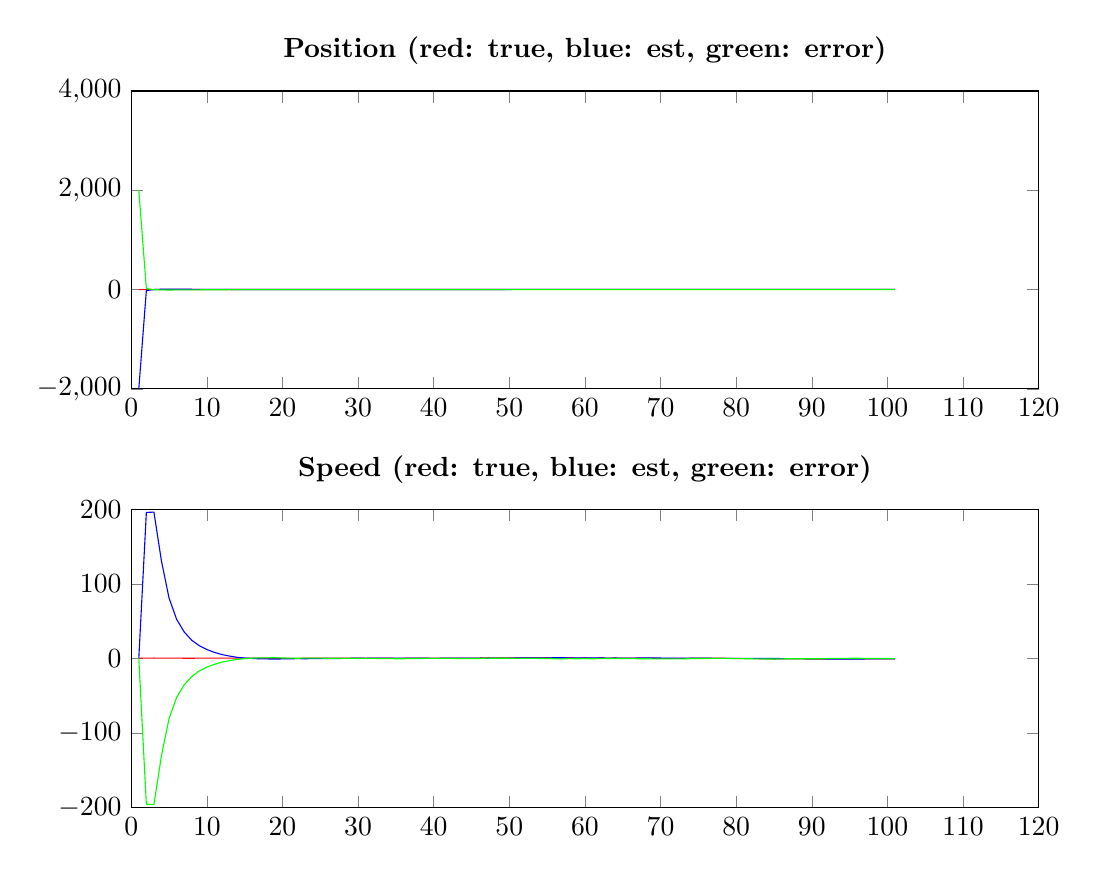
\begin{tikzpicture}

\begin{axis}[%
width=4.537in,
height=1.49in,
at={(0.761in,2.579in)},
scale only axis,
xmin=0,
xmax=120,
ymin=-2000,
ymax=4000,
axis background/.style={fill=white},
title style={font=\bfseries},
title={Position (red: true, blue: est, green: error)}
]
\addplot [color=red,solid,forget plot]
  table[row sep=crcr]{%
1	1\\
2	1.03893818149443\\
3	1.09834065175243\\
4	1.15785523402398\\
5	1.21540556958781\\
6	1.26450909867691\\
7	1.31650727707921\\
8	1.35580798656931\\
9	1.37785647878524\\
10	1.45506244887376\\
11	1.5062824671877\\
12	1.55793127373411\\
13	1.62051205019349\\
14	1.677144622592\\
15	1.71361123251335\\
16	1.74520797684153\\
17	1.79260160485084\\
18	1.84266228740054\\
19	1.89219017547123\\
20	1.9526536591475\\
21	1.98194676030208\\
22	1.99714960458363\\
23	2.01183417770998\\
24	2.04578663337777\\
25	2.09625752428472\\
26	2.1343916133339\\
27	2.14741140298422\\
28	2.18861311137538\\
29	2.22372660728145\\
30	2.26285922453739\\
31	2.30534908967932\\
32	2.36762203173353\\
33	2.43436727984676\\
34	2.48367340567866\\
35	2.50726067136607\\
36	2.53265402243325\\
37	2.55658335408082\\
38	2.59179316353207\\
39	2.62748004656853\\
40	2.68617643939315\\
41	2.75313050582855\\
42	2.79850728196857\\
43	2.84661366622812\\
44	2.89534201449348\\
45	2.92647158495399\\
46	2.98506826161624\\
47	3.05254228782199\\
48	3.13068640020582\\
49	3.20835625655959\\
50	3.30695568551287\\
51	3.3843557066642\\
52	3.46044646608772\\
53	3.54446234697186\\
54	3.65073462562676\\
55	3.75251488725988\\
56	3.82823616472618\\
57	3.91873811688683\\
58	4.0043864155827\\
59	4.07225781981238\\
60	4.12912487120948\\
61	4.20910076271691\\
62	4.26771691274636\\
63	4.34510225362229\\
64	4.42053004252639\\
65	4.48972798033486\\
66	4.53068369423004\\
67	4.58231609546513\\
68	4.62163203385248\\
69	4.66116806822613\\
70	4.68903977053571\\
71	4.70719137557682\\
72	4.72560123365852\\
73	4.74650069933502\\
74	4.77499408229755\\
75	4.81458236442016\\
76	4.85958011935162\\
77	4.92291349021385\\
78	4.96090265674736\\
79	4.98904247211309\\
80	5.01903365037247\\
81	5.02835907516912\\
82	5.01710400376678\\
83	5.00382633872209\\
84	4.99326918780636\\
85	4.94535515883022\\
86	4.89960002510707\\
87	4.86167072183919\\
88	4.82710940714814\\
89	4.78832886681066\\
90	4.7366589903168\\
91	4.67420687501545\\
92	4.59811215984765\\
93	4.53411454614506\\
94	4.48963768500242\\
95	4.44636218381481\\
96	4.38905065051708\\
97	4.3707494213093\\
98	4.31892481785098\\
99	4.30159615416602\\
100	4.26215666163003\\
101	4.22250252856481\\
};
\addplot [color=blue,solid,forget plot]
  table[row sep=crcr]{%
1	-2000\\
2	-18.5497041011256\\
3	1.14520686330859\\
4	7.56429154646287\\
5	8.33602487818146\\
6	7.79503750596328\\
7	7.0508664002522\\
8	6.15296428011151\\
9	5.41085823718621\\
10	4.82306744232924\\
11	4.25303122203954\\
12	3.70605281326716\\
13	3.28300973923587\\
14	2.8517249171584\\
15	2.53986801553694\\
16	2.34654545777866\\
17	2.10991150195001\\
18	2.02181131260315\\
19	1.92991410463507\\
20	1.91236586464073\\
21	1.95388338848541\\
22	2.00000430745704\\
23	1.92965612408066\\
24	1.97572001574823\\
25	1.97962263718895\\
26	2.05394544414845\\
27	2.02778130904716\\
28	2.09445651894362\\
29	2.18329152011614\\
30	2.24791386355699\\
31	2.24712778108056\\
32	2.32336694988649\\
33	2.45098305836694\\
34	2.46379290191758\\
35	2.53331281748186\\
36	2.59661658582108\\
37	2.61009411127304\\
38	2.62629382910234\\
39	2.65375395222675\\
40	2.63507242072158\\
41	2.69870613519721\\
42	2.74731784261297\\
43	2.81218821345585\\
44	2.90799486127621\\
45	2.94849464469428\\
46	3.00250696512348\\
47	2.98206195909366\\
48	3.07111786427665\\
49	3.10053714900393\\
50	3.21640559705639\\
51	3.32179987867267\\
52	3.39318616451589\\
53	3.45992832868289\\
54	3.54685436559437\\
55	3.65150132369227\\
56	3.87497555804042\\
57	3.98550154941742\\
58	3.97281797874441\\
59	4.0841263010939\\
60	4.12009705250357\\
61	4.2581394763919\\
62	4.26662072831261\\
63	4.28514518133769\\
64	4.36809085235432\\
65	4.40450339550015\\
66	4.4714347180455\\
67	4.55596446447865\\
68	4.65205086698009\\
69	4.72136515058156\\
70	4.76397931347741\\
71	4.79816106769141\\
72	4.87993233982455\\
73	4.9223363446732\\
74	4.94097805429695\\
75	4.92011860825943\\
76	4.98388766437485\\
77	4.96572297546434\\
78	4.98402551902915\\
79	4.9468785040022\\
80	4.99957459509501\\
81	4.98872070004943\\
82	5.03945737403149\\
83	5.05891266507649\\
84	5.09272754584695\\
85	5.05644507409506\\
86	4.99118412544283\\
87	4.93301677962461\\
88	4.91889167226902\\
89	4.88088030234991\\
90	4.82208284740256\\
91	4.75359659160079\\
92	4.61376014523534\\
93	4.51848850226589\\
94	4.49845852971903\\
95	4.37463320001117\\
96	4.26549731774555\\
97	4.30222668460899\\
98	4.29203697727477\\
99	4.21673129578072\\
100	4.18902806418593\\
101	4.2496129682025\\
};
\addplot [color=green,solid,forget plot]
  table[row sep=crcr]{%
1	2001\\
2	19.58864228262\\
3	-0.0468662115561689\\
4	-6.40643631243889\\
5	-7.12061930859365\\
6	-6.53052840728637\\
7	-5.73435912317299\\
8	-4.7971562935422\\
9	-4.03300175840097\\
10	-3.36800499345549\\
11	-2.74674875485184\\
12	-2.14812153953306\\
13	-1.66249768904237\\
14	-1.1745802945664\\
15	-0.826256783023594\\
16	-0.601337480937132\\
17	-0.317309897099172\\
18	-0.179149025202612\\
19	-0.0377239291638434\\
20	0.0402877945067748\\
21	0.0280633718166721\\
22	-0.00285470287340783\\
23	0.082178053629318\\
24	0.0700666176295406\\
25	0.116634887095767\\
26	0.080446169185453\\
27	0.119630093937059\\
28	0.0941565924317556\\
29	0.040435087165315\\
30	0.0149453609803984\\
31	0.05822130859876\\
32	0.044255081847044\\
33	-0.0166157785201801\\
34	0.0198805037610779\\
35	-0.0260521461157959\\
36	-0.0639625633878289\\
37	-0.0535107571922158\\
38	-0.0345006655702691\\
39	-0.0262739056582237\\
40	0.0511040186715692\\
41	0.0544243706313368\\
42	0.0511894393555981\\
43	0.0344254527722767\\
44	-0.0126528467827325\\
45	-0.0220230597402882\\
46	-0.0174387035072363\\
47	0.070480328728332\\
48	0.0595685359291696\\
49	0.107819107555655\\
50	0.0905500884564794\\
51	0.0625558279915261\\
52	0.0672603015718298\\
53	0.0845340182889687\\
54	0.103880260032388\\
55	0.101013563567613\\
56	-0.0467393933142377\\
57	-0.0667634325305881\\
58	0.0315684368382882\\
59	-0.0118684812815131\\
60	0.00902781870590985\\
61	-0.0490387136749879\\
62	0.00109618443375847\\
63	0.0599570722845959\\
64	0.0524391901720662\\
65	0.0852245848347053\\
66	0.0592489761845361\\
67	0.026351630986472\\
68	-0.0304188331276087\\
69	-0.0601970823554252\\
70	-0.0749395429416992\\
71	-0.0909696921145908\\
72	-0.154331106166026\\
73	-0.175835645338181\\
74	-0.165983971999398\\
75	-0.10553624383927\\
76	-0.124307545023238\\
77	-0.0428094852504834\\
78	-0.0231228622817863\\
79	0.0421639681108923\\
80	0.0194590552774567\\
81	0.0396383751196918\\
82	-0.0223533702647156\\
83	-0.0550863263543961\\
84	-0.099458358040593\\
85	-0.111089915264841\\
86	-0.0915841003357567\\
87	-0.0713460577854148\\
88	-0.0917822651208837\\
89	-0.0925514355392556\\
90	-0.0854238570857513\\
91	-0.0793897165853439\\
92	-0.0156479853876839\\
93	0.0156260438791689\\
94	-0.00882084471661049\\
95	0.0717289838036432\\
96	0.123553332771531\\
97	0.0685227367003076\\
98	0.0268878405762063\\
99	0.0848648583852922\\
100	0.0731285974440983\\
101	-0.0271104396376867\\
};
\end{axis}

\begin{axis}[%
width=4.537in,
height=1.49in,
at={(0.761in,0.486in)},
scale only axis,
xmin=0,
xmax=120,
ymin=-200,
ymax=200,
axis background/.style={fill=white},
title style={font=\bfseries},
title={Speed (red: true, blue: est, green: error)}
]
\addplot [color=red,solid,forget plot]
  table[row sep=crcr]{%
1	0.5\\
2	0.579669502537248\\
3	0.65770963145256\\
4	0.485420903574911\\
5	0.532502190239965\\
6	0.526097144362865\\
7	0.442994812508789\\
8	0.348050508313287\\
9	0.623705658771342\\
10	0.571633975337022\\
11	0.500532436605907\\
12	0.569969477744453\\
13	0.499989596066185\\
14	0.5296704043815\\
15	0.469647106250523\\
16	0.520974117133434\\
17	0.506459294958169\\
18	0.418269606326772\\
19	0.44157284669613\\
20	0.225773780292236\\
21	0.230323678616892\\
22	0.236399786105925\\
23	0.362409003787659\\
24	0.505228996415396\\
25	0.531005907280051\\
26	0.322327646885543\\
27	0.361760513484665\\
28	0.389273141469207\\
29	0.514915905463155\\
30	0.46281329447441\\
31	0.570279127409846\\
32	0.64272805894348\\
33	0.507059087801359\\
34	0.380443878216662\\
35	0.286959758522829\\
36	0.30601322874254\\
37	0.381743463299514\\
38	0.414765794352431\\
39	0.58478700302298\\
40	0.544381705913265\\
41	0.448115281152698\\
42	0.562900898835682\\
43	0.506349660292995\\
44	0.359192319306999\\
45	0.611411665509346\\
46	0.619981563204883\\
47	0.882667155472135\\
48	0.814263583932758\\
49	0.870505237486543\\
50	0.896997111439841\\
51	0.837455424147089\\
52	0.919023446706656\\
53	0.965747041690871\\
54	0.81436316332457\\
55	0.729432275483785\\
56	0.765045504395375\\
57	0.714345611859921\\
58	0.709419881979888\\
59	0.579511697945289\\
60	0.68441254037652\\
61	0.568194747901936\\
62	0.687506940869073\\
63	0.628080236844638\\
64	0.669160167215381\\
65	0.620745255092958\\
66	0.449111134495518\\
67	0.43861369909365\\
68	0.46988083090629\\
69	0.343138648045123\\
70	0.121707824066847\\
71	0.192029364238348\\
72	0.204368228311369\\
73	0.169214230224347\\
74	0.340022880743018\\
75	0.479041856145216\\
76	0.398481279411019\\
77	0.500206302492733\\
78	0.410029148090757\\
79	0.25493132700289\\
80	0.0509327803366418\\
81	-0.0546621136002154\\
82	-0.118429269090964\\
83	-0.203582610553344\\
84	-0.376161872187712\\
85	-0.570645142637215\\
86	-0.448256402582745\\
87	-0.460659098627369\\
88	-0.436788493593962\\
89	-0.501268373942939\\
90	-0.623779622268198\\
91	-0.676199248428036\\
92	-0.485940637526659\\
93	-0.380815051224103\\
94	-0.444619796376899\\
95	-0.394917055863445\\
96	-0.373045649055214\\
97	-0.34101468606578\\
98	-0.287799215285626\\
99	-0.322600932539452\\
100	-0.375225885260307\\
101	-0.349822207634413\\
};
\addplot [color=blue,solid,forget plot]
  table[row sep=crcr]{%
1	0\\
2	196.163775457764\\
3	196.556442551053\\
4	130.585235209499\\
5	81.2078570055752\\
6	52.6847280326677\\
7	35.7775812086346\\
8	24.5753920241516\\
9	17.1750705213009\\
10	12.0920741462076\\
11	8.26371518650116\\
12	5.33568829017622\\
13	3.29775581249015\\
14	1.67197873602635\\
15	0.645130563278696\\
16	0.0909258398275463\\
17	-0.438203740759192\\
18	-0.533642780360589\\
19	-0.616724832124215\\
20	-0.521584534721547\\
21	-0.319624084052748\\
22	-0.151304541942004\\
23	-0.270319893079317\\
24	-0.112782970068954\\
25	-0.0800663926477615\\
26	0.0973592290012882\\
27	0.0199925240515268\\
28	0.15937324805389\\
29	0.316472966377627\\
30	0.3875368451813\\
31	0.302325217893462\\
32	0.401473701001213\\
33	0.589976884866559\\
34	0.490437806696507\\
35	0.534565767830841\\
36	0.555787371017949\\
37	0.465055404565708\\
38	0.399743589925008\\
39	0.372774271209345\\
40	0.252177620589035\\
41	0.334967494451947\\
42	0.367541604533483\\
43	0.428134597143181\\
44	0.542339741747533\\
45	0.512741310241377\\
46	0.518642357724036\\
47	0.36280935758054\\
48	0.476544222137024\\
49	0.43724584044485\\
50	0.592722436445751\\
51	0.692119627896472\\
52	0.696805492058036\\
53	0.690473004748107\\
54	0.729003309694312\\
55	0.797420181802008\\
56	1.10717619498251\\
57	1.10676321893278\\
58	0.840911418084822\\
59	0.899566920374509\\
60	0.783222302703751\\
61	0.911924757693448\\
62	0.733674539138664\\
63	0.615482878566474\\
64	0.661596187586639\\
65	0.597488531060408\\
66	0.612967406692352\\
67	0.663036649564144\\
68	0.727221160801339\\
69	0.719876971514162\\
70	0.656574330625192\\
71	0.588741376730441\\
72	0.638086786360161\\
73	0.591957765374201\\
74	0.504560058578447\\
75	0.350868766210013\\
76	0.412681474638319\\
77	0.284598300673478\\
78	0.26270842340225\\
79	0.126037166347059\\
80	0.21243988386229\\
81	0.143266022436509\\
82	0.221733042303599\\
83	0.21587547640405\\
84	0.24222649264294\\
85	0.111832447639492\\
86	-0.0529117496970754\\
87	-0.166864712445248\\
88	-0.161344740042985\\
89	-0.208491442711165\\
90	-0.290273507551579\\
91	-0.375311040805293\\
92	-0.595788368706618\\
93	-0.672709615810636\\
94	-0.570900982976312\\
95	-0.714721483153377\\
96	-0.795890259237579\\
97	-0.545213531564126\\
98	-0.449674798258072\\
99	-0.515056385257858\\
100	-0.46376003102496\\
101	-0.233249536999796\\
};
\addplot [color=green,solid,forget plot]
  table[row sep=crcr]{%
1	0.5\\
2	-195.584105955227\\
3	-195.8987329196\\
4	-130.099814305924\\
5	-80.6753548153353\\
6	-52.1586308883048\\
7	-35.3345863961259\\
8	-24.2273415158384\\
9	-16.5513648625296\\
10	-11.5204401708706\\
11	-7.76318274989525\\
12	-4.76571881243177\\
13	-2.79776621642397\\
14	-1.14230833164485\\
15	-0.175483457028172\\
16	0.430048277305887\\
17	0.944663035717361\\
18	0.951912386687361\\
19	1.05829767882035\\
20	0.747358315013783\\
21	0.54994776266964\\
22	0.387704328047929\\
23	0.632728896866976\\
24	0.61801196648435\\
25	0.611072299927813\\
26	0.224968417884255\\
27	0.341767989433138\\
28	0.229899893415317\\
29	0.198442939085528\\
30	0.0752764492931101\\
31	0.267953909516384\\
32	0.241254357942267\\
33	-0.0829177970652002\\
34	-0.109993928479845\\
35	-0.247606009308012\\
36	-0.24977414227541\\
37	-0.0833119412661942\\
38	0.0150222044274235\\
39	0.212012731813634\\
40	0.29220408532423\\
41	0.113147786700751\\
42	0.1953592943022\\
43	0.0782150631498132\\
44	-0.183147422440534\\
45	0.0986703552679692\\
46	0.101339205480847\\
47	0.519857797891595\\
48	0.337719361795734\\
49	0.433259397041692\\
50	0.304274674994089\\
51	0.145335796250617\\
52	0.22221795464862\\
53	0.275274036942764\\
54	0.0853598536302584\\
55	-0.067987906318223\\
56	-0.342130690587135\\
57	-0.392417607072859\\
58	-0.131491536104933\\
59	-0.320055222429219\\
60	-0.098809762327231\\
61	-0.343730009791512\\
62	-0.046167598269591\\
63	0.0125973582781639\\
64	0.00756397962874145\\
65	0.02325672403255\\
66	-0.163856272196834\\
67	-0.224422950470495\\
68	-0.257340329895049\\
69	-0.376738323469039\\
70	-0.534866506558345\\
71	-0.396712012492093\\
72	-0.433718558048792\\
73	-0.422743535149855\\
74	-0.164537177835429\\
75	0.128173089935203\\
76	-0.0142001952273005\\
77	0.215608001819256\\
78	0.147320724688506\\
79	0.128894160655831\\
80	-0.161507103525648\\
81	-0.197928136036724\\
82	-0.340162311394563\\
83	-0.419458086957394\\
84	-0.618388364830653\\
85	-0.682477590276707\\
86	-0.39534465288567\\
87	-0.29379438618212\\
88	-0.275443753550977\\
89	-0.292776931231774\\
90	-0.33350611471662\\
91	-0.300888207622743\\
92	0.109847731179959\\
93	0.291894564586533\\
94	0.126281186599413\\
95	0.319804427289932\\
96	0.422844610182365\\
97	0.204198845498346\\
98	0.161875582972446\\
99	0.192455452718406\\
100	0.0885341457646531\\
101	-0.116572670634617\\
};
\end{axis}
\end{tikzpicture}%}
	\scalebox{0.5}{% This file was created by matlab2tikz.
%
%The latest updates can be retrieved from
%  http://www.mathworks.com/matlabcentral/fileexchange/22022-matlab2tikz-matlab2tikz
%where you can also make suggestions and rate matlab2tikz.
%
\definecolor{mycolor1}{rgb}{0.00000,0.44700,0.74100}%
%
\begin{tikzpicture}

\begin{axis}[%
width=4.521in,
height=1.474in,
at={(0.758in,2.554in)},
scale only axis,
xmin=0,
xmax=120,
ymin=0,
ymax=1,
axis background/.style={fill=white},
title style={font=\bfseries},
title={sqrt(P(1,1))}
]
\addplot [color=mycolor1,solid,forget plot]
  table[row sep=crcr]{%
1	1\\
2	0.0995086448257605\\
3	0.0817847279255382\\
4	0.0817858266978378\\
5	0.07928330010311\\
6	0.0755371114415577\\
7	0.0718817684944784\\
8	0.0687508084368571\\
9	0.0662394232116604\\
10	0.0643269395836851\\
11	0.0629460736742048\\
12	0.0620067630964009\\
13	0.0614098333927467\\
14	0.061059059985402\\
15	0.0608711204341967\\
16	0.060781345758464\\
17	0.0607446758425194\\
18	0.0607330012396365\\
19	0.0607308124122334\\
20	0.0607307932898959\\
21	0.0607302777377582\\
22	0.0607288328353198\\
23	0.0607268390357299\\
24	0.0607247873226744\\
25	0.0607230145863017\\
26	0.0607216644609177\\
27	0.0607207377867615\\
28	0.0607201596778544\\
29	0.060719832254771\\
30	0.0607196658077923\\
31	0.060719591887528\\
32	0.0607195648731387\\
33	0.0607195579142109\\
34	0.0607195572542368\\
35	0.0607195570909026\\
36	0.0607195557900676\\
37	0.0607195534957194\\
38	0.0607195508369724\\
39	0.0607195483590311\\
40	0.0607195463611778\\
41	0.0607195449218992\\
42	0.0607195439821046\\
43	0.0607195434240489\\
44	0.0607195431245423\\
45	0.0607195429819021\\
46	0.0607195429240133\\
47	0.0607195429058031\\
48	0.0607195429024946\\
49	0.0607195429024783\\
50	0.060719542901579\\
51	0.0607195428991667\\
52	0.060719542895885\\
53	0.0607195428925334\\
54	0.0607195428896523\\
55	0.0607195428874668\\
56	0.0607195428859721\\
57	0.0607195428850428\\
58	0.0607195428845185\\
59	0.0607195428842531\\
60	0.0607195428841359\\
61	0.0607195428840934\\
62	0.0607195428840827\\
63	0.0607195428840818\\
64	0.0607195428840815\\
65	0.0607195428840793\\
66	0.0607195428840755\\
67	0.0607195428840711\\
68	0.0607195428840671\\
69	0.0607195428840638\\
70	0.0607195428840615\\
71	0.06071954288406\\
72	0.0607195428840591\\
73	0.0607195428840586\\
74	0.0607195428840584\\
75	0.0607195428840583\\
76	0.0607195428840583\\
77	0.0607195428840583\\
78	0.0607195428840583\\
79	0.0607195428840583\\
80	0.0607195428840582\\
81	0.0607195428840582\\
82	0.0607195428840582\\
83	0.0607195428840582\\
84	0.0607195428840582\\
85	0.0607195428840582\\
86	0.0607195428840582\\
87	0.0607195428840582\\
88	0.0607195428840582\\
89	0.0607195428840582\\
90	0.0607195428840582\\
91	0.0607195428840582\\
92	0.0607195428840582\\
93	0.0607195428840582\\
94	0.0607195428840582\\
95	0.0607195428840582\\
96	0.0607195428840582\\
97	0.0607195428840582\\
98	0.0607195428840582\\
99	0.0607195428840582\\
100	0.0607195428840582\\
101	0.0607195428840582\\
};
\end{axis}

\begin{axis}[%
width=4.521in,
height=1.474in,
at={(0.758in,0.481in)},
scale only axis,
xmin=0,
xmax=120,
ymin=0,
ymax=1.5,
axis background/.style={fill=white},
title style={font=\bfseries},
title={sqrt(P(2,2))}
]
\addplot [color=mycolor1,solid,forget plot]
  table[row sep=crcr]{%
1	1\\
2	1.00009851490037\\
3	0.820009501501226\\
4	0.588858415977073\\
5	0.430052722558678\\
6	0.335754955215735\\
7	0.281163607476242\\
8	0.250023838252038\\
9	0.23272861210873\\
10	0.223521735783159\\
11	0.218915649012111\\
12	0.216811049705421\\
13	0.215974085069402\\
14	0.215711641143716\\
15	0.2156629197542\\
16	0.215662517474054\\
17	0.215650894582232\\
18	0.215618478100173\\
19	0.215573810126525\\
20	0.215527880380332\\
21	0.215488221045571\\
22	0.215458034540381\\
23	0.215437327925883\\
24	0.215424417578627\\
25	0.215417109940942\\
26	0.215413397549232\\
27	0.215411750240386\\
28	0.215411148997365\\
29	0.215410994519295\\
30	0.215410980021967\\
31	0.215410976276778\\
32	0.215410947016401\\
33	0.215410895575815\\
34	0.21541083605076\\
35	0.215410780622068\\
36	0.215410735960819\\
37	0.215410703803256\\
38	0.215410682815774\\
39	0.215410670359416\\
40	0.215410663677812\\
41	0.215410660497883\\
42	0.215410659208621\\
43	0.215410658803763\\
44	0.215410658730546\\
45	0.215410658730221\\
46	0.215410658709911\\
47	0.215410658655764\\
48	0.215410658582249\\
49	0.215410658507249\\
50	0.215410658442824\\
51	0.215410658393982\\
52	0.215410658360594\\
53	0.215410658339847\\
54	0.215410658328146\\
55	0.215410658322228\\
56	0.215410658319616\\
57	0.215410658318672\\
58	0.215410658318434\\
59	0.215410658318413\\
60	0.215410658318406\\
61	0.215410658318357\\
62	0.215410658318271\\
63	0.215410658318174\\
64	0.215410658318083\\
65	0.215410658318011\\
66	0.215410658317959\\
67	0.215410658317925\\
68	0.215410658317905\\
69	0.215410658317895\\
70	0.21541065831789\\
71	0.215410658317887\\
72	0.215410658317887\\
73	0.215410658317887\\
74	0.215410658317887\\
75	0.215410658317887\\
76	0.215410658317887\\
77	0.215410658317886\\
78	0.215410658317886\\
79	0.215410658317886\\
80	0.215410658317886\\
81	0.215410658317886\\
82	0.215410658317886\\
83	0.215410658317886\\
84	0.215410658317886\\
85	0.215410658317886\\
86	0.215410658317886\\
87	0.215410658317886\\
88	0.215410658317886\\
89	0.215410658317886\\
90	0.215410658317886\\
91	0.215410658317886\\
92	0.215410658317886\\
93	0.215410658317886\\
94	0.215410658317886\\
95	0.215410658317886\\
96	0.215410658317886\\
97	0.215410658317886\\
98	0.215410658317886\\
99	0.215410658317886\\
100	0.215410658317886\\
101	0.215410658317886\\
};
\end{axis}
\end{tikzpicture}%}
	\scalebox{0.5}{% This file was created by matlab2tikz.
%
%The latest updates can be retrieved from
%  http://www.mathworks.com/matlabcentral/fileexchange/22022-matlab2tikz-matlab2tikz
%where you can also make suggestions and rate matlab2tikz.
%
\definecolor{mycolor1}{rgb}{0.00000,0.44700,0.74100}%
%
\begin{tikzpicture}

\begin{axis}[%
width=4.521in,
height=1.474in,
at={(0.758in,2.554in)},
scale only axis,
xmin=0,
xmax=100,
ymin=0.2,
ymax=1,
axis background/.style={fill=white},
title style={font=\bfseries},
title={K(1)}
]
\addplot [color=mycolor1,solid,forget plot]
  table[row sep=crcr]{%
1	0.990197039505931\\
2	0.668874172185431\\
3	0.668892144864875\\
4	0.628584167523981\\
5	0.570585520493431\\
6	0.516698864189379\\
7	0.472667366072143\\
8	0.438766118741346\\
9	0.413795515620307\\
10	0.396220819099841\\
11	0.384483866969318\\
12	0.37711676373249\\
13	0.372820880630092\\
14	0.370529330291448\\
15	0.369437199220995\\
16	0.368991564321276\\
17	0.368849743957369\\
18	0.368823157624988\\
19	0.368822925362007\\
20	0.368816663410525\\
21	0.368799113754021\\
22	0.368774897927145\\
23	0.368749979538404\\
24	0.368728450044821\\
25	0.368712053490428\\
26	0.368700799736865\\
27	0.368693779130414\\
28	0.368689802904753\\
29	0.368687781580998\\
30	0.368686883898796\\
31	0.36868655583833\\
32	0.368686471329721\\
33	0.368686463315054\\
34	0.368686461331538\\
35	0.368686445534313\\
36	0.368686417671953\\
37	0.368686385384368\\
38	0.368686355292471\\
39	0.368686331030722\\
40	0.368686313552253\\
41	0.368686302139473\\
42	0.368686295362496\\
43	0.368686291725314\\
44	0.368686289993106\\
45	0.368686289290109\\
46	0.368686289068966\\
47	0.368686289028788\\
48	0.36868628902859\\
49	0.368686289017669\\
50	0.368686288988375\\
51	0.368686288948522\\
52	0.36868628890782\\
53	0.368686288872832\\
54	0.368686288846292\\
55	0.36868628882814\\
56	0.368686288816855\\
57	0.368686288810488\\
58	0.368686288807265\\
59	0.368686288805841\\
60	0.368686288805326\\
61	0.368686288805196\\
62	0.368686288805184\\
63	0.368686288805181\\
64	0.368686288805154\\
65	0.368686288805108\\
66	0.368686288805055\\
67	0.368686288805006\\
68	0.368686288804967\\
69	0.368686288804938\\
70	0.36868628880492\\
71	0.368686288804909\\
72	0.368686288804903\\
73	0.3686862888049\\
74	0.368686288804899\\
75	0.368686288804899\\
76	0.368686288804899\\
77	0.368686288804899\\
78	0.368686288804899\\
79	0.368686288804899\\
80	0.368686288804899\\
81	0.368686288804899\\
82	0.368686288804899\\
83	0.368686288804899\\
84	0.368686288804899\\
85	0.368686288804899\\
86	0.368686288804899\\
87	0.368686288804899\\
88	0.368686288804899\\
89	0.368686288804899\\
90	0.368686288804899\\
91	0.368686288804899\\
92	0.368686288804899\\
93	0.368686288804899\\
94	0.368686288804899\\
95	0.368686288804899\\
96	0.368686288804899\\
97	0.368686288804899\\
98	0.368686288804899\\
99	0.368686288804899\\
100	0.368686288804899\\
};
\end{axis}

\begin{axis}[%
width=4.521in,
height=1.474in,
at={(0.758in,0.481in)},
scale only axis,
xmin=0,
xmax=100,
ymin=0,
ymax=4,
axis background/.style={fill=white},
title style={font=\bfseries},
title={K(2)}
]
\addplot [color=mycolor1,solid,forget plot]
  table[row sep=crcr]{%
1	0.0980296049406921\\
2	3.34437086092715\\
3	3.33376827552124\\
4	2.52611444444076\\
5	1.8789322064163\\
6	1.45292215752488\\
7	1.18304539910372\\
8	1.01480323419368\\
9	0.912385837117251\\
10	0.852539524694961\\
11	0.819732160908219\\
12	0.803396338934124\\
13	0.796419888232492\\
14	0.794225181413138\\
15	0.79408673449753\\
16	0.794559479896688\\
17	0.795004791802089\\
18	0.795231110831293\\
19	0.795252683075777\\
20	0.795149212103974\\
21	0.794998113467713\\
22	0.794851121505177\\
23	0.794733388001474\\
24	0.79465105651638\\
25	0.794599846108912\\
26	0.794571585005714\\
27	0.794558099542126\\
28	0.794552955206301\\
29	0.794551831362776\\
30	0.794552212232882\\
31	0.794552855382299\\
32	0.79455328818786\\
33	0.794553431600915\\
34	0.79455336273753\\
35	0.794553188388173\\
36	0.794552991914607\\
37	0.794552821051145\\
38	0.794552693973016\\
39	0.794552610402752\\
40	0.794552561468725\\
41	0.794552536290912\\
42	0.794552525418535\\
43	0.794552522031155\\
44	0.794552521873623\\
45	0.794552522658058\\
46	0.794552523376367\\
47	0.794552523733141\\
48	0.794552523758676\\
49	0.794552523584555\\
50	0.794552523336274\\
51	0.794552523096846\\
52	0.79455252290611\\
53	0.794552522773302\\
54	0.794552522691036\\
55	0.794552522645847\\
56	0.79455252262442\\
57	0.794552522616339\\
58	0.794552522614645\\
59	0.794552522615311\\
60	0.794552522616361\\
61	0.794552522617052\\
62	0.794552522617271\\
63	0.794552522617149\\
64	0.79455252261686\\
65	0.794552522616539\\
66	0.794552522616261\\
67	0.794552522616056\\
68	0.794552522615921\\
69	0.794552522615843\\
70	0.794552522615803\\
71	0.794552522615785\\
72	0.79455252261578\\
73	0.79455252261578\\
74	0.794552522615782\\
75	0.794552522615783\\
76	0.794552522615783\\
77	0.794552522615783\\
78	0.794552522615783\\
79	0.794552522615782\\
80	0.794552522615782\\
81	0.794552522615782\\
82	0.794552522615781\\
83	0.794552522615781\\
84	0.794552522615781\\
85	0.794552522615781\\
86	0.794552522615781\\
87	0.794552522615781\\
88	0.794552522615781\\
89	0.794552522615781\\
90	0.794552522615781\\
91	0.794552522615781\\
92	0.794552522615781\\
93	0.794552522615781\\
94	0.794552522615781\\
95	0.794552522615781\\
96	0.794552522615781\\
97	0.794552522615781\\
98	0.794552522615781\\
99	0.794552522615781\\
100	0.794552522615781\\
};
\end{axis}
\end{tikzpicture}%}

	\caption{$\hat{x}_0' = \hat{x}_0 \times 1000$}
	\label{fig:q4:xhat1000}
\end{figure}

\begin{figure}[H]
	\scalebox{0.5}{% This file was created by matlab2tikz.
%
%The latest updates can be retrieved from
%  http://www.mathworks.com/matlabcentral/fileexchange/22022-matlab2tikz-matlab2tikz
%where you can also make suggestions and rate matlab2tikz.
%
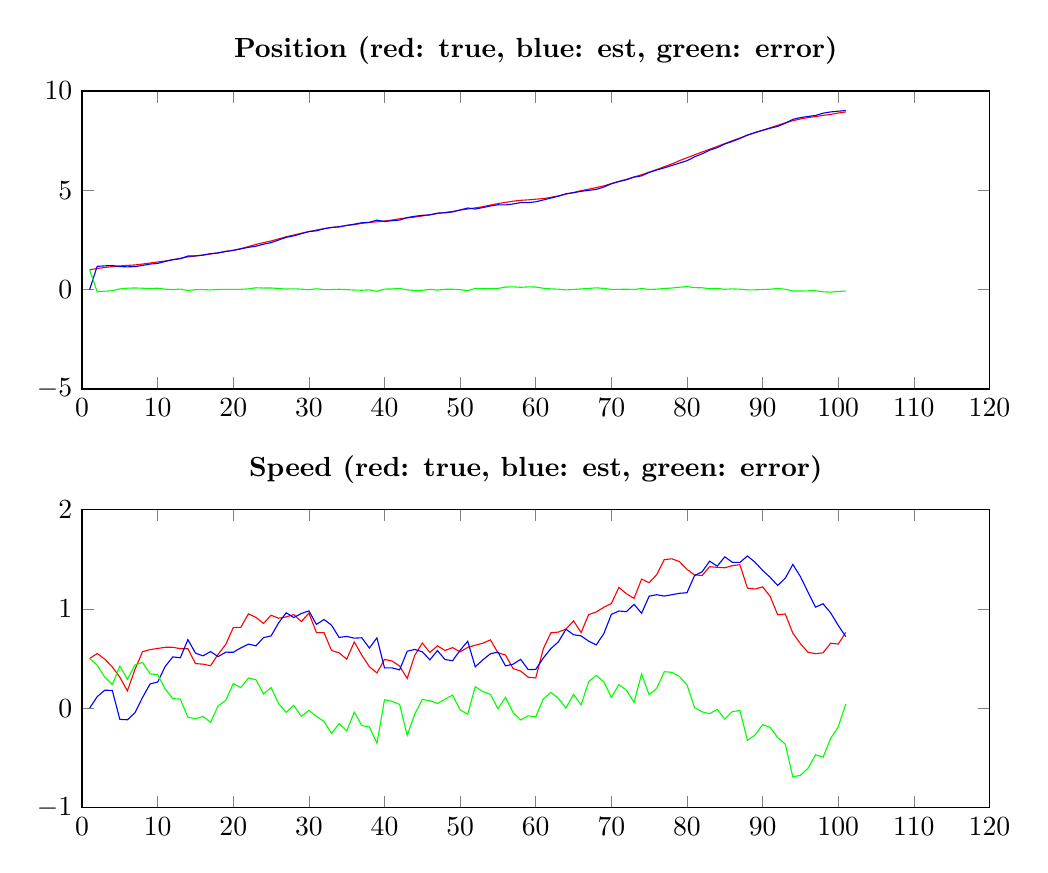
\begin{tikzpicture}

\begin{axis}[%
width=4.537in,
height=1.49in,
at={(0.761in,2.579in)},
scale only axis,
xmin=0,
xmax=120,
ymin=-5,
ymax=10,
axis background/.style={fill=white},
title style={font=\bfseries},
title={Position (red: true, blue: est, green: error)}
]
\addplot [color=red,solid,forget plot]
  table[row sep=crcr]{%
1	1\\
2	1.06024314611482\\
3	1.1161601806454\\
4	1.15878437405725\\
5	1.194568392396\\
6	1.21937481109196\\
7	1.2421111477531\\
8	1.28721330343654\\
9	1.34033512097129\\
10	1.39112518615007\\
11	1.44030617421675\\
12	1.50762188168493\\
13	1.57976907518721\\
14	1.64683326470649\\
15	1.69373762180272\\
16	1.74005490736085\\
17	1.79376381765038\\
18	1.85286209950081\\
19	1.92946554170594\\
20	1.98294276709926\\
21	2.06295817048959\\
22	2.16653392533846\\
23	2.27740155913941\\
24	2.36430130655653\\
25	2.44899995975432\\
26	2.55264961845116\\
27	2.66162014638954\\
28	2.74662440650995\\
29	2.83917117993574\\
30	2.91754878724986\\
31	3.00047916470462\\
32	3.06730520354262\\
33	3.13125786581206\\
34	3.17229028542593\\
35	3.23246488650104\\
36	3.27215246453518\\
37	3.33607019339882\\
38	3.37854692709867\\
39	3.41363882140926\\
40	3.45564323565748\\
41	3.50196254305605\\
42	3.56603514930988\\
43	3.61162803399146\\
44	3.65168913111165\\
45	3.7070040788063\\
46	3.77246475369341\\
47	3.82831002459223\\
48	3.8845953285479\\
49	3.93021896879552\\
50	4.00461162082291\\
51	4.05621581217709\\
52	4.11559644754386\\
53	4.17429638350547\\
54	4.25633182866698\\
55	4.33037192014938\\
56	4.3912301492062\\
57	4.45202407456876\\
58	4.49615933427797\\
59	4.51781213344503\\
60	4.55258557868863\\
61	4.58108439345405\\
62	4.64491223688647\\
63	4.72095457762278\\
64	4.80833346126916\\
65	4.88691790254526\\
66	4.9833991784136\\
67	5.05453790008409\\
68	5.13637174453966\\
69	5.2227734066343\\
70	5.33777442255591\\
71	5.45116532005937\\
72	5.55199830499002\\
73	5.66910994859258\\
74	5.78209056262728\\
75	5.91216347907723\\
76	6.04390763919748\\
77	6.18746859432545\\
78	6.32812219545261\\
79	6.49081350128844\\
80	6.63926215748239\\
81	6.78300981060979\\
82	6.92885105984026\\
83	7.06584310774985\\
84	7.20793771612035\\
85	7.34839890563621\\
86	7.49761216322468\\
87	7.62729658968014\\
88	7.77325105188003\\
89	7.89724886713419\\
90	8.02317942783886\\
91	8.14548257297819\\
92	8.27340586186078\\
93	8.39385965166822\\
94	8.50233648525639\\
95	8.58842888950628\\
96	8.65781964402045\\
97	8.70899111536487\\
98	8.76986724857803\\
99	8.8181393100119\\
100	8.89006572329681\\
101	8.94129824626566\\
};
\addplot [color=blue,solid,forget plot]
  table[row sep=crcr]{%
1	-0.002\\
2	1.17090886367798\\
3	1.19554467794368\\
4	1.21323698809764\\
5	1.15868488941634\\
6	1.14614950894334\\
7	1.15975915990143\\
8	1.2168572760761\\
9	1.28626393448253\\
10	1.31944431011087\\
11	1.41886607943726\\
12	1.50590764986326\\
13	1.5535786527201\\
14	1.68988061720289\\
15	1.69541023710531\\
16	1.73807453425787\\
17	1.81092622781949\\
18	1.84440863165727\\
19	1.91712134510455\\
20	1.97290423214774\\
21	2.04998748363108\\
22	2.12837000321237\\
23	2.18475041414646\\
24	2.28600917965266\\
25	2.36499325208594\\
26	2.49901019048449\\
27	2.63174094785467\\
28	2.70566434979272\\
29	2.81585282665214\\
30	2.92327699228603\\
31	2.95810403853528\\
32	3.06575314540901\\
33	3.1279565479729\\
34	3.15439266752835\\
35	3.23058594998288\\
36	3.29471542034545\\
37	3.36703097793706\\
38	3.38996838222133\\
39	3.49816202615895\\
40	3.42843446730335\\
41	3.46923662000371\\
42	3.50068263961431\\
43	3.62596775212667\\
44	3.69206220480605\\
45	3.73993024248646\\
46	3.75921260918442\\
47	3.85149306377885\\
48	3.86776587835484\\
49	3.91076474449092\\
50	4.00773933356386\\
51	4.1078242073177\\
52	4.05613075247775\\
53	4.13009034417853\\
54	4.20728818275796\\
55	4.27001725838478\\
56	4.26212790379897\\
57	4.31250035817875\\
58	4.37944600083171\\
59	4.3808667589226\\
60	4.42058902138858\\
61	4.51265597832843\\
62	4.60752916989532\\
63	4.69902922991474\\
64	4.82473686229547\\
65	4.87869880575648\\
66	4.94727201186126\\
67	4.99546561363662\\
68	5.04551916473523\\
69	5.16155456072549\\
70	5.32681276597188\\
71	5.43706205121643\\
72	5.53194506244013\\
73	5.66346531895609\\
74	5.72616488421956\\
75	5.90179054582881\\
76	6.02131125723183\\
77	6.12918822727944\\
78	6.24842269176075\\
79	6.3692360446279\\
80	6.48785850758758\\
81	6.68404684783332\\
82	6.83518459765298\\
83	7.02234840789389\\
84	7.14683725499604\\
85	7.33363978022856\\
86	7.46046696478189\\
87	7.60682958674939\\
88	7.78372175963611\\
89	7.90771022129455\\
90	8.01664718914249\\
91	8.12305822568648\\
92	8.21667943430415\\
93	8.37462304654091\\
94	8.56930754629389\\
95	8.65768353177815\\
96	8.7178284346047\\
97	8.76441184809221\\
98	8.88161058447371\\
99	8.94443939214953\\
100	8.98195020773528\\
101	9.01260077583703\\
};
\addplot [color=green,solid,forget plot]
  table[row sep=crcr]{%
1	1.002\\
2	-0.110665717563164\\
3	-0.0793844972982856\\
4	-0.0544526140403943\\
5	0.0358835029796616\\
6	0.0732253021486173\\
7	0.0823519878516634\\
8	0.0703560273604378\\
9	0.0540711864887609\\
10	0.0716808760391996\\
11	0.0214400947794922\\
12	0.00171423182166386\\
13	0.0261904224671112\\
14	-0.0430473524963964\\
15	-0.00167261530258345\\
16	0.0019803731029775\\
17	-0.0171624101691175\\
18	0.00845346784353596\\
19	0.0123441966013851\\
20	0.0100385349515233\\
21	0.0129706868585036\\
22	0.038163922126095\\
23	0.0926511449929484\\
24	0.0782921269038734\\
25	0.0840067076683821\\
26	0.0536394279666688\\
27	0.0298791985348719\\
28	0.0409600567172341\\
29	0.0233183532836017\\
30	-0.005728205036172\\
31	0.0423751261693477\\
32	0.00155205813361192\\
33	0.00330131783916432\\
34	0.0178976178975727\\
35	0.00187893651816751\\
36	-0.0225629558102711\\
37	-0.0309607845382418\\
38	-0.0114214551226559\\
39	-0.0845232047496811\\
40	0.0272087683541309\\
41	0.0327259230523378\\
42	0.06535250969557\\
43	-0.0143397181352172\\
44	-0.0403730736944006\\
45	-0.0329261636801554\\
46	0.0132521445089866\\
47	-0.0231830391866175\\
48	0.0168294501930624\\
49	0.0194542243045994\\
50	-0.00312771274094903\\
51	-0.051608395140617\\
52	0.059465695066117\\
53	0.0442060393269363\\
54	0.0490436459090189\\
55	0.060354661764606\\
56	0.129102245407227\\
57	0.13952371639001\\
58	0.116713333446256\\
59	0.136945374522435\\
60	0.131996557300049\\
61	0.0684284151256191\\
62	0.0373830669911497\\
63	0.0219253477080423\\
64	-0.0164034010263094\\
65	0.00821909678878008\\
66	0.0361271665523466\\
67	0.0590722864474653\\
68	0.0908525798044231\\
69	0.0612188459088046\\
70	0.0109616565840245\\
71	0.0141032688429386\\
72	0.0200532425498894\\
73	0.00564462963648626\\
74	0.055925678407724\\
75	0.0103729332484157\\
76	0.0225963819656458\\
77	0.0582803670460059\\
78	0.0796995036918551\\
79	0.121577456660535\\
80	0.151403649894807\\
81	0.0989629627764756\\
82	0.0936664621872794\\
83	0.0434946998559589\\
84	0.0611004611243091\\
85	0.0147591254076449\\
86	0.0371451984427864\\
87	0.0204670029307552\\
88	-0.0104707077560784\\
89	-0.0104613541603609\\
90	0.00653223869637287\\
91	0.0224243472917127\\
92	0.0567264275566295\\
93	0.0192366051273094\\
94	-0.0669710610374992\\
95	-0.069254642271865\\
96	-0.0600087905842486\\
97	-0.0554207327273382\\
98	-0.111743335895683\\
99	-0.126300082137629\\
100	-0.0918844844384683\\
101	-0.0713025295713745\\
};
\end{axis}

\begin{axis}[%
width=4.537in,
height=1.49in,
at={(0.761in,0.486in)},
scale only axis,
xmin=0,
xmax=120,
ymin=-1,
ymax=2,
axis background/.style={fill=white},
title style={font=\bfseries},
title={Speed (red: true, blue: est, green: error)}
]
\addplot [color=red,solid,forget plot]
  table[row sep=crcr]{%
1	0.5\\
2	0.550968010552678\\
3	0.494077670765353\\
4	0.416009178004766\\
5	0.311797091381084\\
6	0.174663423750642\\
7	0.391160073213985\\
8	0.569166412795878\\
9	0.590161000611961\\
10	0.601530531057634\\
11	0.613381466262182\\
12	0.613556136235118\\
13	0.599476505877544\\
14	0.598639215388712\\
15	0.449294407618228\\
16	0.443484904775966\\
17	0.428237239589244\\
18	0.544051916066859\\
19	0.641250397798432\\
20	0.811539511219388\\
21	0.814477437913219\\
22	0.949731299057166\\
23	0.914561063109613\\
24	0.853855102701426\\
25	0.93647443108855\\
26	0.90583704822613\\
27	0.919431898613781\\
28	0.942631994325417\\
29	0.871868879596129\\
30	0.957580392307252\\
31	0.761635772673447\\
32	0.760523792546461\\
33	0.581243159197877\\
34	0.557276150941421\\
35	0.49337114565535\\
36	0.666867622610629\\
37	0.53421348958878\\
38	0.417442671395423\\
39	0.355229793829668\\
40	0.490854369964785\\
41	0.475870187486302\\
42	0.424131178718429\\
43	0.299623891427499\\
44	0.532692344385645\\
45	0.656552719360922\\
46	0.562156970192523\\
47	0.628348911854946\\
48	0.581087899584328\\
49	0.610328026512999\\
50	0.567208939983524\\
51	0.612370347522627\\
52	0.634142118897859\\
53	0.654133220604194\\
54	0.688191003850468\\
55	0.558924067383858\\
56	0.535630959789682\\
57	0.39878911483555\\
58	0.374491253554018\\
59	0.312260270113903\\
60	0.304727551790526\\
61	0.598432648800918\\
62	0.759452627683861\\
63	0.766702676928086\\
64	0.796785894548727\\
65	0.87951010635698\\
66	0.761998094391694\\
67	0.942367362995434\\
68	0.96902386217255\\
69	1.01589044360847\\
70	1.05395018781886\\
71	1.21680624154382\\
72	1.15209479337816\\
73	1.10534055905672\\
74	1.29998341358534\\
75	1.26363786693077\\
76	1.34432033033908\\
77	1.49678350521747\\
78	1.50382288883592\\
79	1.47636699489813\\
80	1.3977920213749\\
81	1.34136332243145\\
82	1.33678214651532\\
83	1.42500092520797\\
84	1.41798656769842\\
85	1.41390652335963\\
86	1.435370385567\\
87	1.4444577991475\\
88	1.20891597594215\\
89	1.19983793604923\\
90	1.2218572552116\\
91	1.12635683482507\\
92	0.939522144097721\\
93	0.949014660586912\\
94	0.754900009374743\\
95	0.650220887614992\\
96	0.563642238056241\\
97	0.54879400795895\\
98	0.558203401009696\\
99	0.654955140742752\\
100	0.645836497426907\\
101	0.763164503249588\\
};
\addplot [color=blue,solid,forget plot]
  table[row sep=crcr]{%
1	0\\
2	0.116118093622214\\
3	0.181238118139609\\
4	0.179087507527733\\
5	-0.112113588314215\\
6	-0.116473577860029\\
7	-0.0454525824981172\\
8	0.108835434261173\\
9	0.244191023082561\\
10	0.263508926226992\\
11	0.420733906568859\\
12	0.516607534413926\\
13	0.508107909573152\\
14	0.690734136808468\\
15	0.554528775949031\\
16	0.527040363564656\\
17	0.570424856810494\\
18	0.519644347219539\\
19	0.564380357953858\\
20	0.562967732091481\\
21	0.607782279431355\\
22	0.645730794271336\\
23	0.628072456416944\\
24	0.710943529912264\\
25	0.727946757868993\\
26	0.859884946461263\\
27	0.960617230757663\\
28	0.912907767333221\\
29	0.953633665808026\\
30	0.979625658095485\\
31	0.843563137490914\\
32	0.893761212234734\\
33	0.835201501914726\\
34	0.712180135674052\\
35	0.72290229946196\\
36	0.705315112231807\\
37	0.70915989552678\\
38	0.605761663896072\\
39	0.70838166738375\\
40	0.405449730928147\\
41	0.406003976389466\\
42	0.386275458572614\\
43	0.573030402541264\\
44	0.591976696644058\\
45	0.567560308215427\\
46	0.486801150016293\\
47	0.580763851832535\\
48	0.490673350733196\\
49	0.477595247606184\\
50	0.583658192479772\\
51	0.673566553649902\\
52	0.417002726152903\\
53	0.486524496117675\\
54	0.548042408506399\\
55	0.565121149034074\\
56	0.426330118297897\\
57	0.443009321697449\\
58	0.491810734672164\\
59	0.38888290628478\\
60	0.390680191530807\\
61	0.504897728209253\\
62	0.600548036880245\\
63	0.668315427480589\\
64	0.795198761523402\\
65	0.740119089429882\\
66	0.728398189599644\\
67	0.675283347438196\\
68	0.637623597539512\\
69	0.750276750280765\\
70	0.944731758722529\\
71	0.978730710892543\\
72	0.972286859626332\\
73	1.04618831654225\\
74	0.95584848056694\\
75	1.12834372178287\\
76	1.14275339162792\\
77	1.12896432358969\\
78	1.14262335991444\\
79	1.15674139777575\\
80	1.16309530268884\\
81	1.33524141144809\\
82	1.37320034192619\\
83	1.48061821776919\\
84	1.42981631093911\\
85	1.52425432786124\\
86	1.46908777210502\\
87	1.4679107578269\\
88	1.53278136290158\\
89	1.46965944713773\\
90	1.38770353931379\\
91	1.31796626390923\\
92	1.23569476259582\\
93	1.309774155518\\
94	1.44706872273564\\
95	1.32567053257047\\
96	1.16959420408986\\
97	1.01792750118008\\
98	1.05112880434956\\
99	0.960002777433426\\
100	0.833952660803384\\
101	0.720283034060997\\
};
\addplot [color=green,solid,forget plot]
  table[row sep=crcr]{%
1	0.5\\
2	0.434849916930464\\
3	0.312839552625744\\
4	0.236921670477033\\
5	0.423910679695299\\
6	0.291137001610672\\
7	0.436612655712103\\
8	0.460330978534704\\
9	0.3459699775294\\
10	0.338021604830643\\
11	0.192647559693323\\
12	0.0969486018211917\\
13	0.0913685963043919\\
14	-0.0920949214197559\\
15	-0.105234368330803\\
16	-0.0835554587886901\\
17	-0.14218761722125\\
18	0.0244075688473199\\
19	0.0768700398445743\\
20	0.248571779127907\\
21	0.206695158481864\\
22	0.304000504785831\\
23	0.286488606692669\\
24	0.142911572789161\\
25	0.208527673219557\\
26	0.0459521017648672\\
27	-0.0411853321438818\\
28	0.0297242269921959\\
29	-0.0817647862118971\\
30	-0.0220452657882332\\
31	-0.0819273648174672\\
32	-0.133237419688273\\
33	-0.253958342716849\\
34	-0.15490398473263\\
35	-0.22953115380661\\
36	-0.0384474896211775\\
37	-0.174946405938\\
38	-0.188318992500649\\
39	-0.353151873554082\\
40	0.0854046390366382\\
41	0.0698662110968361\\
42	0.0378557201458147\\
43	-0.273406511113765\\
44	-0.0592843522584133\\
45	0.0889924111454954\\
46	0.0753558201762307\\
47	0.0475850600224106\\
48	0.0904145488511323\\
49	0.132732778906816\\
50	-0.0164492524962483\\
51	-0.0611962061272751\\
52	0.217139392744956\\
53	0.16760872448652\\
54	0.14014859534407\\
55	-0.00619708165021637\\
56	0.109300841491786\\
57	-0.0442202068618988\\
58	-0.117319481118146\\
59	-0.0766226361708773\\
60	-0.0859526397402819\\
61	0.0935349205916655\\
62	0.158904590803616\\
63	0.0983872494474973\\
64	0.00158713302532465\\
65	0.139391016927098\\
66	0.0335999047920502\\
67	0.267084015557237\\
68	0.331400264633039\\
69	0.265613693327704\\
70	0.109218429096332\\
71	0.238075530651275\\
72	0.179807933751824\\
73	0.0591522425144713\\
74	0.3441349330184\\
75	0.135294145147899\\
76	0.201566938711154\\
77	0.36781918162778\\
78	0.361199528921476\\
79	0.319625597122382\\
80	0.234696718686066\\
81	0.00612191098335746\\
82	-0.0364181954108644\\
83	-0.0556172925612213\\
84	-0.0118297432406929\\
85	-0.11034780450161\\
86	-0.0337173865380131\\
87	-0.0234529586793932\\
88	-0.323865386959423\\
89	-0.269821511088494\\
90	-0.165846284102192\\
91	-0.191609429084153\\
92	-0.2961726184981\\
93	-0.360759494931085\\
94	-0.692168713360898\\
95	-0.675449644955481\\
96	-0.605951966033614\\
97	-0.46913349322113\\
98	-0.49292540333986\\
99	-0.305047636690675\\
100	-0.188116163376477\\
101	0.0428814691885914\\
};
\end{axis}
\end{tikzpicture}%}
	\scalebox{0.5}{% This file was created by matlab2tikz.
%
%The latest updates can be retrieved from
%  http://www.mathworks.com/matlabcentral/fileexchange/22022-matlab2tikz-matlab2tikz
%where you can also make suggestions and rate matlab2tikz.
%
\definecolor{mycolor1}{rgb}{0.00000,0.44700,0.74100}%
%
\begin{tikzpicture}

\begin{axis}[%
width=4.521in,
height=1.474in,
at={(0.758in,2.554in)},
scale only axis,
xmin=0,
xmax=120,
ymin=0,
ymax=1,
axis background/.style={fill=white},
title style={font=\bfseries},
title={sqrt(P(1,1))}
]
\addplot [color=mycolor1,solid,forget plot]
  table[row sep=crcr]{%
1	1\\
2	0.0995086448257605\\
3	0.0817847279255382\\
4	0.0817858266978378\\
5	0.07928330010311\\
6	0.0755371114415577\\
7	0.0718817684944784\\
8	0.0687508084368571\\
9	0.0662394232116604\\
10	0.0643269395836851\\
11	0.0629460736742048\\
12	0.0620067630964009\\
13	0.0614098333927467\\
14	0.061059059985402\\
15	0.0608711204341967\\
16	0.060781345758464\\
17	0.0607446758425194\\
18	0.0607330012396365\\
19	0.0607308124122334\\
20	0.0607307932898959\\
21	0.0607302777377582\\
22	0.0607288328353198\\
23	0.0607268390357299\\
24	0.0607247873226744\\
25	0.0607230145863017\\
26	0.0607216644609177\\
27	0.0607207377867615\\
28	0.0607201596778544\\
29	0.060719832254771\\
30	0.0607196658077923\\
31	0.060719591887528\\
32	0.0607195648731387\\
33	0.0607195579142109\\
34	0.0607195572542368\\
35	0.0607195570909026\\
36	0.0607195557900676\\
37	0.0607195534957194\\
38	0.0607195508369724\\
39	0.0607195483590311\\
40	0.0607195463611778\\
41	0.0607195449218992\\
42	0.0607195439821046\\
43	0.0607195434240489\\
44	0.0607195431245423\\
45	0.0607195429819021\\
46	0.0607195429240133\\
47	0.0607195429058031\\
48	0.0607195429024946\\
49	0.0607195429024783\\
50	0.060719542901579\\
51	0.0607195428991667\\
52	0.060719542895885\\
53	0.0607195428925334\\
54	0.0607195428896523\\
55	0.0607195428874668\\
56	0.0607195428859721\\
57	0.0607195428850428\\
58	0.0607195428845185\\
59	0.0607195428842531\\
60	0.0607195428841359\\
61	0.0607195428840934\\
62	0.0607195428840827\\
63	0.0607195428840818\\
64	0.0607195428840815\\
65	0.0607195428840793\\
66	0.0607195428840755\\
67	0.0607195428840711\\
68	0.0607195428840671\\
69	0.0607195428840638\\
70	0.0607195428840615\\
71	0.06071954288406\\
72	0.0607195428840591\\
73	0.0607195428840586\\
74	0.0607195428840584\\
75	0.0607195428840583\\
76	0.0607195428840583\\
77	0.0607195428840583\\
78	0.0607195428840583\\
79	0.0607195428840583\\
80	0.0607195428840582\\
81	0.0607195428840582\\
82	0.0607195428840582\\
83	0.0607195428840582\\
84	0.0607195428840582\\
85	0.0607195428840582\\
86	0.0607195428840582\\
87	0.0607195428840582\\
88	0.0607195428840582\\
89	0.0607195428840582\\
90	0.0607195428840582\\
91	0.0607195428840582\\
92	0.0607195428840582\\
93	0.0607195428840582\\
94	0.0607195428840582\\
95	0.0607195428840582\\
96	0.0607195428840582\\
97	0.0607195428840582\\
98	0.0607195428840582\\
99	0.0607195428840582\\
100	0.0607195428840582\\
101	0.0607195428840582\\
};
\end{axis}

\begin{axis}[%
width=4.521in,
height=1.474in,
at={(0.758in,0.481in)},
scale only axis,
xmin=0,
xmax=120,
ymin=0,
ymax=1.5,
axis background/.style={fill=white},
title style={font=\bfseries},
title={sqrt(P(2,2))}
]
\addplot [color=mycolor1,solid,forget plot]
  table[row sep=crcr]{%
1	1\\
2	1.00009851490037\\
3	0.820009501501226\\
4	0.588858415977073\\
5	0.430052722558678\\
6	0.335754955215735\\
7	0.281163607476242\\
8	0.250023838252038\\
9	0.23272861210873\\
10	0.223521735783159\\
11	0.218915649012111\\
12	0.216811049705421\\
13	0.215974085069402\\
14	0.215711641143716\\
15	0.2156629197542\\
16	0.215662517474054\\
17	0.215650894582232\\
18	0.215618478100173\\
19	0.215573810126525\\
20	0.215527880380332\\
21	0.215488221045571\\
22	0.215458034540381\\
23	0.215437327925883\\
24	0.215424417578627\\
25	0.215417109940942\\
26	0.215413397549232\\
27	0.215411750240386\\
28	0.215411148997365\\
29	0.215410994519295\\
30	0.215410980021967\\
31	0.215410976276778\\
32	0.215410947016401\\
33	0.215410895575815\\
34	0.21541083605076\\
35	0.215410780622068\\
36	0.215410735960819\\
37	0.215410703803256\\
38	0.215410682815774\\
39	0.215410670359416\\
40	0.215410663677812\\
41	0.215410660497883\\
42	0.215410659208621\\
43	0.215410658803763\\
44	0.215410658730546\\
45	0.215410658730221\\
46	0.215410658709911\\
47	0.215410658655764\\
48	0.215410658582249\\
49	0.215410658507249\\
50	0.215410658442824\\
51	0.215410658393982\\
52	0.215410658360594\\
53	0.215410658339847\\
54	0.215410658328146\\
55	0.215410658322228\\
56	0.215410658319616\\
57	0.215410658318672\\
58	0.215410658318434\\
59	0.215410658318413\\
60	0.215410658318406\\
61	0.215410658318357\\
62	0.215410658318271\\
63	0.215410658318174\\
64	0.215410658318083\\
65	0.215410658318011\\
66	0.215410658317959\\
67	0.215410658317925\\
68	0.215410658317905\\
69	0.215410658317895\\
70	0.21541065831789\\
71	0.215410658317887\\
72	0.215410658317887\\
73	0.215410658317887\\
74	0.215410658317887\\
75	0.215410658317887\\
76	0.215410658317887\\
77	0.215410658317886\\
78	0.215410658317886\\
79	0.215410658317886\\
80	0.215410658317886\\
81	0.215410658317886\\
82	0.215410658317886\\
83	0.215410658317886\\
84	0.215410658317886\\
85	0.215410658317886\\
86	0.215410658317886\\
87	0.215410658317886\\
88	0.215410658317886\\
89	0.215410658317886\\
90	0.215410658317886\\
91	0.215410658317886\\
92	0.215410658317886\\
93	0.215410658317886\\
94	0.215410658317886\\
95	0.215410658317886\\
96	0.215410658317886\\
97	0.215410658317886\\
98	0.215410658317886\\
99	0.215410658317886\\
100	0.215410658317886\\
101	0.215410658317886\\
};
\end{axis}
\end{tikzpicture}%}
	\scalebox{0.5}{% This file was created by matlab2tikz.
%
%The latest updates can be retrieved from
%  http://www.mathworks.com/matlabcentral/fileexchange/22022-matlab2tikz-matlab2tikz
%where you can also make suggestions and rate matlab2tikz.
%
\definecolor{mycolor1}{rgb}{0.00000,0.44700,0.74100}%
%
\begin{tikzpicture}

\begin{axis}[%
width=4.521in,
height=1.474in,
at={(0.758in,2.554in)},
scale only axis,
xmin=0,
xmax=100,
ymin=0.2,
ymax=1,
axis background/.style={fill=white},
title style={font=\bfseries},
title={K(1)}
]
\addplot [color=mycolor1,solid,forget plot]
  table[row sep=crcr]{%
1	0.990197039505931\\
2	0.668874172185431\\
3	0.668892144864875\\
4	0.628584167523981\\
5	0.570585520493431\\
6	0.516698864189379\\
7	0.472667366072143\\
8	0.438766118741346\\
9	0.413795515620307\\
10	0.396220819099841\\
11	0.384483866969318\\
12	0.37711676373249\\
13	0.372820880630092\\
14	0.370529330291448\\
15	0.369437199220995\\
16	0.368991564321276\\
17	0.368849743957369\\
18	0.368823157624988\\
19	0.368822925362007\\
20	0.368816663410525\\
21	0.368799113754021\\
22	0.368774897927145\\
23	0.368749979538404\\
24	0.368728450044821\\
25	0.368712053490428\\
26	0.368700799736865\\
27	0.368693779130414\\
28	0.368689802904753\\
29	0.368687781580998\\
30	0.368686883898796\\
31	0.36868655583833\\
32	0.368686471329721\\
33	0.368686463315054\\
34	0.368686461331538\\
35	0.368686445534313\\
36	0.368686417671953\\
37	0.368686385384368\\
38	0.368686355292471\\
39	0.368686331030722\\
40	0.368686313552253\\
41	0.368686302139473\\
42	0.368686295362496\\
43	0.368686291725314\\
44	0.368686289993106\\
45	0.368686289290109\\
46	0.368686289068966\\
47	0.368686289028788\\
48	0.36868628902859\\
49	0.368686289017669\\
50	0.368686288988375\\
51	0.368686288948522\\
52	0.36868628890782\\
53	0.368686288872832\\
54	0.368686288846292\\
55	0.36868628882814\\
56	0.368686288816855\\
57	0.368686288810488\\
58	0.368686288807265\\
59	0.368686288805841\\
60	0.368686288805326\\
61	0.368686288805196\\
62	0.368686288805184\\
63	0.368686288805181\\
64	0.368686288805154\\
65	0.368686288805108\\
66	0.368686288805055\\
67	0.368686288805006\\
68	0.368686288804967\\
69	0.368686288804938\\
70	0.36868628880492\\
71	0.368686288804909\\
72	0.368686288804903\\
73	0.3686862888049\\
74	0.368686288804899\\
75	0.368686288804899\\
76	0.368686288804899\\
77	0.368686288804899\\
78	0.368686288804899\\
79	0.368686288804899\\
80	0.368686288804899\\
81	0.368686288804899\\
82	0.368686288804899\\
83	0.368686288804899\\
84	0.368686288804899\\
85	0.368686288804899\\
86	0.368686288804899\\
87	0.368686288804899\\
88	0.368686288804899\\
89	0.368686288804899\\
90	0.368686288804899\\
91	0.368686288804899\\
92	0.368686288804899\\
93	0.368686288804899\\
94	0.368686288804899\\
95	0.368686288804899\\
96	0.368686288804899\\
97	0.368686288804899\\
98	0.368686288804899\\
99	0.368686288804899\\
100	0.368686288804899\\
};
\end{axis}

\begin{axis}[%
width=4.521in,
height=1.474in,
at={(0.758in,0.481in)},
scale only axis,
xmin=0,
xmax=100,
ymin=0,
ymax=4,
axis background/.style={fill=white},
title style={font=\bfseries},
title={K(2)}
]
\addplot [color=mycolor1,solid,forget plot]
  table[row sep=crcr]{%
1	0.0980296049406921\\
2	3.34437086092715\\
3	3.33376827552124\\
4	2.52611444444076\\
5	1.8789322064163\\
6	1.45292215752488\\
7	1.18304539910372\\
8	1.01480323419368\\
9	0.912385837117251\\
10	0.852539524694961\\
11	0.819732160908219\\
12	0.803396338934124\\
13	0.796419888232492\\
14	0.794225181413138\\
15	0.79408673449753\\
16	0.794559479896688\\
17	0.795004791802089\\
18	0.795231110831293\\
19	0.795252683075777\\
20	0.795149212103974\\
21	0.794998113467713\\
22	0.794851121505177\\
23	0.794733388001474\\
24	0.79465105651638\\
25	0.794599846108912\\
26	0.794571585005714\\
27	0.794558099542126\\
28	0.794552955206301\\
29	0.794551831362776\\
30	0.794552212232882\\
31	0.794552855382299\\
32	0.79455328818786\\
33	0.794553431600915\\
34	0.79455336273753\\
35	0.794553188388173\\
36	0.794552991914607\\
37	0.794552821051145\\
38	0.794552693973016\\
39	0.794552610402752\\
40	0.794552561468725\\
41	0.794552536290912\\
42	0.794552525418535\\
43	0.794552522031155\\
44	0.794552521873623\\
45	0.794552522658058\\
46	0.794552523376367\\
47	0.794552523733141\\
48	0.794552523758676\\
49	0.794552523584555\\
50	0.794552523336274\\
51	0.794552523096846\\
52	0.79455252290611\\
53	0.794552522773302\\
54	0.794552522691036\\
55	0.794552522645847\\
56	0.79455252262442\\
57	0.794552522616339\\
58	0.794552522614645\\
59	0.794552522615311\\
60	0.794552522616361\\
61	0.794552522617052\\
62	0.794552522617271\\
63	0.794552522617149\\
64	0.79455252261686\\
65	0.794552522616539\\
66	0.794552522616261\\
67	0.794552522616056\\
68	0.794552522615921\\
69	0.794552522615843\\
70	0.794552522615803\\
71	0.794552522615785\\
72	0.79455252261578\\
73	0.79455252261578\\
74	0.794552522615782\\
75	0.794552522615783\\
76	0.794552522615783\\
77	0.794552522615783\\
78	0.794552522615783\\
79	0.794552522615782\\
80	0.794552522615782\\
81	0.794552522615782\\
82	0.794552522615781\\
83	0.794552522615781\\
84	0.794552522615781\\
85	0.794552522615781\\
86	0.794552522615781\\
87	0.794552522615781\\
88	0.794552522615781\\
89	0.794552522615781\\
90	0.794552522615781\\
91	0.794552522615781\\
92	0.794552522615781\\
93	0.794552522615781\\
94	0.794552522615781\\
95	0.794552522615781\\
96	0.794552522615781\\
97	0.794552522615781\\
98	0.794552522615781\\
99	0.794552522615781\\
100	0.794552522615781\\
};
\end{axis}
\end{tikzpicture}%}

	\caption{$\hat{x}_0' = \hat{x}_0 \times 0.001$}
	\label{fig:q4:xhat001}
\end{figure}
